%%%%%%%% ICML 2019 EXAMPLE LATEX SUBMISSION FILE %%%%%%%%%%%%%%%%%

\documentclass{article}

% Recommended, but optional, packages for figures and better typesetting:
\usepackage{microtype}
\usepackage{graphicx}
\usepackage{subcaption}
\usepackage{booktabs} % for professional tables
\usepackage{multicol}
\usepackage[dvipsnames]{xcolor}

% hyperref makes hyperlinks in the resulting PDF.
% If your build breaks (sometimes temporarily if a hyperlink spans a page)
% please comment out the following usepackage line and replace
% \usepackage{icml2019} with \usepackage[nohyperref]{icml2019} above.
\usepackage{hyperref}
%%%%% NEW MATH DEFINITIONS %%%%%

\usepackage{amsmath,amsfonts,bm}

% Mark sections of captions for referring to divisions of figures
\newcommand{\figleft}{{\em (Left)}}
\newcommand{\figcenter}{{\em (Center)}}
\newcommand{\figright}{{\em (Right)}}
\newcommand{\figtop}{{\em (Top)}}
\newcommand{\figbottom}{{\em (Bottom)}}
\newcommand{\captiona}{{\em (a)}}
\newcommand{\captionb}{{\em (b)}}
\newcommand{\captionc}{{\em (c)}}
\newcommand{\captiond}{{\em (d)}}

% Highlight a newly defined term
\newcommand{\newterm}[1]{{\bf #1}}


% Figure reference, lower-case.
\def\figref#1{figure~\ref{#1}}
% Figure reference, capital. For start of sentence
\def\Figref#1{Figure~\ref{#1}}
\def\twofigref#1#2{figures \ref{#1} and \ref{#2}}
\def\quadfigref#1#2#3#4{figures \ref{#1}, \ref{#2}, \ref{#3} and \ref{#4}}
% Section reference, lower-case.
\def\secref#1{section~\ref{#1}}
% Section reference, capital.
\def\Secref#1{Section~\ref{#1}}
% Reference to two sections.
\def\twosecrefs#1#2{sections \ref{#1} and \ref{#2}}
% Reference to three sections.
\def\secrefs#1#2#3{sections \ref{#1}, \ref{#2} and \ref{#3}}
% Reference to an equation, lower-case.
\def\eqref#1{equation~\ref{#1}}
% Reference to an equation, upper case
\def\Eqref#1{Equation~\ref{#1}}
% A raw reference to an equation---avoid using if possible
\def\plaineqref#1{\ref{#1}}
% Reference to a chapter, lower-case.
\def\chapref#1{chapter~\ref{#1}}
% Reference to an equation, upper case.
\def\Chapref#1{Chapter~\ref{#1}}
% Reference to a range of chapters
\def\rangechapref#1#2{chapters\ref{#1}--\ref{#2}}
% Reference to an algorithm, lower-case.
\def\algref#1{algorithm~\ref{#1}}
% Reference to an algorithm, upper case.
\def\Algref#1{Algorithm~\ref{#1}}
\def\twoalgref#1#2{algorithms \ref{#1} and \ref{#2}}
\def\Twoalgref#1#2{Algorithms \ref{#1} and \ref{#2}}
% Reference to a part, lower case
\def\partref#1{part~\ref{#1}}
% Reference to a part, upper case
\def\Partref#1{Part~\ref{#1}}
\def\twopartref#1#2{parts \ref{#1} and \ref{#2}}

\def\ceil#1{\lceil #1 \rceil}
\def\floor#1{\lfloor #1 \rfloor}
\def\1{\bm{1}}
\newcommand{\train}{\mathcal{D}}
\newcommand{\valid}{\mathcal{D_{\mathrm{valid}}}}
\newcommand{\test}{\mathcal{D_{\mathrm{test}}}}

\def\eps{{\epsilon}}


% Random variables
\def\reta{{\textnormal{$\eta$}}}
\def\ra{{\textnormal{a}}}
\def\rb{{\textnormal{b}}}
\def\rc{{\textnormal{c}}}
\def\rd{{\textnormal{d}}}
\def\re{{\textnormal{e}}}
\def\rf{{\textnormal{f}}}
\def\rg{{\textnormal{g}}}
\def\rh{{\textnormal{h}}}
\def\ri{{\textnormal{i}}}
\def\rj{{\textnormal{j}}}
\def\rk{{\textnormal{k}}}
\def\rl{{\textnormal{l}}}
% rm is already a command, just don't name any random variables m
\def\rn{{\textnormal{n}}}
\def\ro{{\textnormal{o}}}
\def\rp{{\textnormal{p}}}
\def\rq{{\textnormal{q}}}
\def\rr{{\textnormal{r}}}
\def\rs{{\textnormal{s}}}
\def\rt{{\textnormal{t}}}
\def\ru{{\textnormal{u}}}
\def\rv{{\textnormal{v}}}
\def\rw{{\textnormal{w}}}
\def\rx{{\textnormal{x}}}
\def\ry{{\textnormal{y}}}
\def\rz{{\textnormal{z}}}

% Random vectors
\def\rvepsilon{{\mathbf{\epsilon}}}
\def\rvtheta{{\mathbf{\theta}}}
\def\rva{{\mathbf{a}}}
\def\rvb{{\mathbf{b}}}
\def\rvc{{\mathbf{c}}}
\def\rvd{{\mathbf{d}}}
\def\rve{{\mathbf{e}}}
\def\rvf{{\mathbf{f}}}
\def\rvg{{\mathbf{g}}}
\def\rvh{{\mathbf{h}}}
\def\rvu{{\mathbf{i}}}
\def\rvj{{\mathbf{j}}}
\def\rvk{{\mathbf{k}}}
\def\rvl{{\mathbf{l}}}
\def\rvm{{\mathbf{m}}}
\def\rvn{{\mathbf{n}}}
\def\rvo{{\mathbf{o}}}
\def\rvp{{\mathbf{p}}}
\def\rvq{{\mathbf{q}}}
\def\rvr{{\mathbf{r}}}
\def\rvs{{\mathbf{s}}}
\def\rvt{{\mathbf{t}}}
\def\rvu{{\mathbf{u}}}
\def\rvv{{\mathbf{v}}}
\def\rvw{{\mathbf{w}}}
\def\rvx{{\mathbf{x}}}
\def\rvy{{\mathbf{y}}}
\def\rvz{{\mathbf{z}}}

% Elements of random vectors
\def\erva{{\textnormal{a}}}
\def\ervb{{\textnormal{b}}}
\def\ervc{{\textnormal{c}}}
\def\ervd{{\textnormal{d}}}
\def\erve{{\textnormal{e}}}
\def\ervf{{\textnormal{f}}}
\def\ervg{{\textnormal{g}}}
\def\ervh{{\textnormal{h}}}
\def\ervi{{\textnormal{i}}}
\def\ervj{{\textnormal{j}}}
\def\ervk{{\textnormal{k}}}
\def\ervl{{\textnormal{l}}}
\def\ervm{{\textnormal{m}}}
\def\ervn{{\textnormal{n}}}
\def\ervo{{\textnormal{o}}}
\def\ervp{{\textnormal{p}}}
\def\ervq{{\textnormal{q}}}
\def\ervr{{\textnormal{r}}}
\def\ervs{{\textnormal{s}}}
\def\ervt{{\textnormal{t}}}
\def\ervu{{\textnormal{u}}}
\def\ervv{{\textnormal{v}}}
\def\ervw{{\textnormal{w}}}
\def\ervx{{\textnormal{x}}}
\def\ervy{{\textnormal{y}}}
\def\ervz{{\textnormal{z}}}

% Random matrices
\def\rmA{{\mathbf{A}}}
\def\rmB{{\mathbf{B}}}
\def\rmC{{\mathbf{C}}}
\def\rmD{{\mathbf{D}}}
\def\rmE{{\mathbf{E}}}
\def\rmF{{\mathbf{F}}}
\def\rmG{{\mathbf{G}}}
\def\rmH{{\mathbf{H}}}
\def\rmI{{\mathbf{I}}}
\def\rmJ{{\mathbf{J}}}
\def\rmK{{\mathbf{K}}}
\def\rmL{{\mathbf{L}}}
\def\rmM{{\mathbf{M}}}
\def\rmN{{\mathbf{N}}}
\def\rmO{{\mathbf{O}}}
\def\rmP{{\mathbf{P}}}
\def\rmQ{{\mathbf{Q}}}
\def\rmR{{\mathbf{R}}}
\def\rmS{{\mathbf{S}}}
\def\rmT{{\mathbf{T}}}
\def\rmU{{\mathbf{U}}}
\def\rmV{{\mathbf{V}}}
\def\rmW{{\mathbf{W}}}
\def\rmX{{\mathbf{X}}}
\def\rmY{{\mathbf{Y}}}
\def\rmZ{{\mathbf{Z}}}

% Elements of random matrices
\def\ermA{{\textnormal{A}}}
\def\ermB{{\textnormal{B}}}
\def\ermC{{\textnormal{C}}}
\def\ermD{{\textnormal{D}}}
\def\ermE{{\textnormal{E}}}
\def\ermF{{\textnormal{F}}}
\def\ermG{{\textnormal{G}}}
\def\ermH{{\textnormal{H}}}
\def\ermI{{\textnormal{I}}}
\def\ermJ{{\textnormal{J}}}
\def\ermK{{\textnormal{K}}}
\def\ermL{{\textnormal{L}}}
\def\ermM{{\textnormal{M}}}
\def\ermN{{\textnormal{N}}}
\def\ermO{{\textnormal{O}}}
\def\ermP{{\textnormal{P}}}
\def\ermQ{{\textnormal{Q}}}
\def\ermR{{\textnormal{R}}}
\def\ermS{{\textnormal{S}}}
\def\ermT{{\textnormal{T}}}
\def\ermU{{\textnormal{U}}}
\def\ermV{{\textnormal{V}}}
\def\ermW{{\textnormal{W}}}
\def\ermX{{\textnormal{X}}}
\def\ermY{{\textnormal{Y}}}
\def\ermZ{{\textnormal{Z}}}

% Vectors
\def\vzero{{\bm{0}}}
\def\vone{{\bm{1}}}
\def\vmu{{\bm{\mu}}}
\def\vtheta{{\bm{\theta}}}
\def\va{{\bm{a}}}
\def\vb{{\bm{b}}}
\def\vc{{\bm{c}}}
\def\vd{{\bm{d}}}
\def\ve{{\bm{e}}}
\def\vf{{\bm{f}}}
\def\vg{{\bm{g}}}
\def\vh{{\bm{h}}}
\def\vi{{\bm{i}}}
\def\vj{{\bm{j}}}
\def\vk{{\bm{k}}}
\def\vl{{\bm{l}}}
\def\vm{{\bm{m}}}
\def\vn{{\bm{n}}}
\def\vo{{\bm{o}}}
\def\vp{{\bm{p}}}
\def\vq{{\bm{q}}}
\def\vr{{\bm{r}}}
\def\vs{{\bm{s}}}
\def\vt{{\bm{t}}}
\def\vu{{\bm{u}}}
\def\vv{{\bm{v}}}
\def\vw{{\bm{w}}}
\def\vx{{\bm{x}}}
\def\vy{{\bm{y}}}
\def\vz{{\bm{z}}}

% Elements of vectors
\def\evalpha{{\alpha}}
\def\evbeta{{\beta}}
\def\evepsilon{{\epsilon}}
\def\evlambda{{\lambda}}
\def\evomega{{\omega}}
\def\evmu{{\mu}}
\def\evpsi{{\psi}}
\def\evsigma{{\sigma}}
\def\evtheta{{\theta}}
\def\eva{{a}}
\def\evb{{b}}
\def\evc{{c}}
\def\evd{{d}}
\def\eve{{e}}
\def\evf{{f}}
\def\evg{{g}}
\def\evh{{h}}
\def\evi{{i}}
\def\evj{{j}}
\def\evk{{k}}
\def\evl{{l}}
\def\evm{{m}}
\def\evn{{n}}
\def\evo{{o}}
\def\evp{{p}}
\def\evq{{q}}
\def\evr{{r}}
\def\evs{{s}}
\def\evt{{t}}
\def\evu{{u}}
\def\evv{{v}}
\def\evw{{w}}
\def\evx{{x}}
\def\evy{{y}}
\def\evz{{z}}

% Matrix
\def\mA{{\bm{A}}}
\def\mB{{\bm{B}}}
\def\mC{{\bm{C}}}
\def\mD{{\bm{D}}}
\def\mE{{\bm{E}}}
\def\mF{{\bm{F}}}
\def\mG{{\bm{G}}}
\def\mH{{\bm{H}}}
\def\mI{{\bm{I}}}
\def\mJ{{\bm{J}}}
\def\mK{{\bm{K}}}
\def\mL{{\bm{L}}}
\def\mM{{\bm{M}}}
\def\mN{{\bm{N}}}
\def\mO{{\bm{O}}}
\def\mP{{\bm{P}}}
\def\mQ{{\bm{Q}}}
\def\mR{{\bm{R}}}
\def\mS{{\bm{S}}}
\def\mT{{\bm{T}}}
\def\mU{{\bm{U}}}
\def\mV{{\bm{V}}}
\def\mW{{\bm{W}}}
\def\mX{{\bm{X}}}
\def\mY{{\bm{Y}}}
\def\mZ{{\bm{Z}}}
\def\mBeta{{\bm{\beta}}}
\def\mPhi{{\bm{\Phi}}}
\def\mLambda{{\bm{\Lambda}}}
\def\mSigma{{\bm{\Sigma}}}

% Tensor
\DeclareMathAlphabet{\mathsfit}{\encodingdefault}{\sfdefault}{m}{sl}
\SetMathAlphabet{\mathsfit}{bold}{\encodingdefault}{\sfdefault}{bx}{n}
\newcommand{\tens}[1]{\bm{\mathsfit{#1}}}
\def\tA{{\tens{A}}}
\def\tB{{\tens{B}}}
\def\tC{{\tens{C}}}
\def\tD{{\tens{D}}}
\def\tE{{\tens{E}}}
\def\tF{{\tens{F}}}
\def\tG{{\tens{G}}}
\def\tH{{\tens{H}}}
\def\tI{{\tens{I}}}
\def\tJ{{\tens{J}}}
\def\tK{{\tens{K}}}
\def\tL{{\tens{L}}}
\def\tM{{\tens{M}}}
\def\tN{{\tens{N}}}
\def\tO{{\tens{O}}}
\def\tP{{\tens{P}}}
\def\tQ{{\tens{Q}}}
\def\tR{{\tens{R}}}
\def\tS{{\tens{S}}}
\def\tT{{\tens{T}}}
\def\tU{{\tens{U}}}
\def\tV{{\tens{V}}}
\def\tW{{\tens{W}}}
\def\tX{{\tens{X}}}
\def\tY{{\tens{Y}}}
\def\tZ{{\tens{Z}}}


% Graph
\def\gA{{\mathcal{A}}}
\def\gB{{\mathcal{B}}}
\def\gC{{\mathcal{C}}}
\def\gD{{\mathcal{D}}}
\def\gE{{\mathcal{E}}}
\def\gF{{\mathcal{F}}}
\def\gG{{\mathcal{G}}}
\def\gH{{\mathcal{H}}}
\def\gI{{\mathcal{I}}}
\def\gJ{{\mathcal{J}}}
\def\gK{{\mathcal{K}}}
\def\gL{{\mathcal{L}}}
\def\gM{{\mathcal{M}}}
\def\gN{{\mathcal{N}}}
\def\gO{{\mathcal{O}}}
\def\gP{{\mathcal{P}}}
\def\gQ{{\mathcal{Q}}}
\def\gR{{\mathcal{R}}}
\def\gS{{\mathcal{S}}}
\def\gT{{\mathcal{T}}}
\def\gU{{\mathcal{U}}}
\def\gV{{\mathcal{V}}}
\def\gW{{\mathcal{W}}}
\def\gX{{\mathcal{X}}}
\def\gY{{\mathcal{Y}}}
\def\gZ{{\mathcal{Z}}}

% Sets
\def\sA{{\mathbb{A}}}
\def\sB{{\mathbb{B}}}
\def\sC{{\mathbb{C}}}
\def\sD{{\mathbb{D}}}
% Don't use a set called E, because this would be the same as our symbol
% for expectation.
\def\sF{{\mathbb{F}}}
\def\sG{{\mathbb{G}}}
\def\sH{{\mathbb{H}}}
\def\sI{{\mathbb{I}}}
\def\sJ{{\mathbb{J}}}
\def\sK{{\mathbb{K}}}
\def\sL{{\mathbb{L}}}
\def\sM{{\mathbb{M}}}
\def\sN{{\mathbb{N}}}
\def\sO{{\mathbb{O}}}
\def\sP{{\mathbb{P}}}
\def\sQ{{\mathbb{Q}}}
\def\sR{{\mathbb{R}}}
\def\sS{{\mathbb{S}}}
\def\sT{{\mathbb{T}}}
\def\sU{{\mathbb{U}}}
\def\sV{{\mathbb{V}}}
\def\sW{{\mathbb{W}}}
\def\sX{{\mathbb{X}}}
\def\sY{{\mathbb{Y}}}
\def\sZ{{\mathbb{Z}}}

% Entries of a matrix
\def\emLambda{{\Lambda}}
\def\emA{{A}}
\def\emB{{B}}
\def\emC{{C}}
\def\emD{{D}}
\def\emE{{E}}
\def\emF{{F}}
\def\emG{{G}}
\def\emH{{H}}
\def\emI{{I}}
\def\emJ{{J}}
\def\emK{{K}}
\def\emL{{L}}
\def\emM{{M}}
\def\emN{{N}}
\def\emO{{O}}
\def\emP{{P}}
\def\emQ{{Q}}
\def\emR{{R}}
\def\emS{{S}}
\def\emT{{T}}
\def\emU{{U}}
\def\emV{{V}}
\def\emW{{W}}
\def\emX{{X}}
\def\emY{{Y}}
\def\emZ{{Z}}
\def\emSigma{{\Sigma}}

% entries of a tensor
% Same font as tensor, without \bm wrapper
\newcommand{\etens}[1]{\mathsfit{#1}}
\def\etLambda{{\etens{\Lambda}}}
\def\etA{{\etens{A}}}
\def\etB{{\etens{B}}}
\def\etC{{\etens{C}}}
\def\etD{{\etens{D}}}
\def\etE{{\etens{E}}}
\def\etF{{\etens{F}}}
\def\etG{{\etens{G}}}
\def\etH{{\etens{H}}}
\def\etI{{\etens{I}}}
\def\etJ{{\etens{J}}}
\def\etK{{\etens{K}}}
\def\etL{{\etens{L}}}
\def\etM{{\etens{M}}}
\def\etN{{\etens{N}}}
\def\etO{{\etens{O}}}
\def\etP{{\etens{P}}}
\def\etQ{{\etens{Q}}}
\def\etR{{\etens{R}}}
\def\etS{{\etens{S}}}
\def\etT{{\etens{T}}}
\def\etU{{\etens{U}}}
\def\etV{{\etens{V}}}
\def\etW{{\etens{W}}}
\def\etX{{\etens{X}}}
\def\etY{{\etens{Y}}}
\def\etZ{{\etens{Z}}}

% The true underlying data generating distribution
\newcommand{\pdata}{p_{\rm{data}}}
% The empirical distribution defined by the training set
\newcommand{\ptrain}{\hat{p}_{\rm{data}}}
\newcommand{\Ptrain}{\hat{P}_{\rm{data}}}
% The model distribution
\newcommand{\pmodel}{p_{\rm{model}}}
\newcommand{\Pmodel}{P_{\rm{model}}}
\newcommand{\ptildemodel}{\tilde{p}_{\rm{model}}}
% Stochastic autoencoder distributions
\newcommand{\pencode}{p_{\rm{encoder}}}
\newcommand{\pdecode}{p_{\rm{decoder}}}
\newcommand{\precons}{p_{\rm{reconstruct}}}

\newcommand{\laplace}{\mathrm{Laplace}} % Laplace distribution

\newcommand{\E}{\mathbb{E}}
\newcommand{\Ls}{\mathcal{L}}
\newcommand{\R}{\mathbb{R}}
\newcommand{\emp}{\tilde{p}}
\newcommand{\lr}{\alpha}
\newcommand{\reg}{\lambda}
\newcommand{\rect}{\mathrm{rectifier}}
\newcommand{\softmax}{\mathrm{softmax}}
\newcommand{\sigmoid}{\sigma}
\newcommand{\softplus}{\zeta}
\newcommand{\KL}{D_{\mathrm{KL}}}
\newcommand{\Var}{\mathrm{Var}}
\newcommand{\standarderror}{\mathrm{SE}}
\newcommand{\Cov}{\mathrm{Cov}}
% Wolfram Mathworld says $L^2$ is for function spaces and $\ell^2$ is for vectors
% But then they seem to use $L^2$ for vectors throughout the site, and so does
% wikipedia.
\newcommand{\normlzero}{L^0}
\newcommand{\normlone}{L^1}
\newcommand{\normltwo}{L^2}
\newcommand{\normlp}{L^p}
\newcommand{\normmax}{L^\infty}
\newcommand{\gradlossktj}{\frac{\partial L_{k+1}(\bW_{N:1}(k, t))}{\partial \bW_j(k, t)}}

\newcommand{\parents}{Pa} % See usage in notation.tex. Chosen to match Daphne's book.

\DeclareMathOperator*{\argmax}{arg\,max}
\DeclareMathOperator*{\argmin}{arg\,min}

\DeclareMathOperator{\sign}{sign}
\DeclareMathOperator{\Tr}{Tr}
\let\ab\allowbreak

\usepackage{semicrunch}
\usepackage{wrapfig,lipsum,booktabs}

% Attempt to make hyperref and algorithmic work together better:
\newcommand{\theHalgorithm}{\arabic{algorithm}}

\usepackage{amsthm}
\newtheorem{theorem}{Theorem}[section]
\newtheorem{proposition}{Proposition}[section]
\newtheorem{corollary}{Corollary}[theorem]
\newtheorem{lemma}{Lemma}[theorem]
\newtheorem{corollaryp}{Corollary}[proposition]
\newtheorem{definition}{Definition}[section]


% Use the following line for the initial blind version submitted for review:
 %\usepackage{icml2019}

% If accepted, instead use the following line for the camera-ready submission:
\usepackage[accepted]{icml2019}

% The \icmltitle you define below is probably too long as a header.
% Therefore, a short form for the running title is supplied here:
%\icmltitlerunning{Diagnosing Bottlenecks in Deep Q-learning Algorithms}

\begin{document}

\twocolumn[
\icmltitle{Diagnosing Bottlenecks in Deep Q-learning Algorithms}

% It is OKAY to include author information, even for blind
% submissions: the style file will automatically remove it for you
% unless you've provided the [accepted] option to the icml2019
% package.

% List of affiliations: The first argument should be a (short)
% identifier you will use later to specify author affiliations
% Academic affiliations should list Department, University, City, Region, Country
% Industry affiliations should list Company, City, Region, Country

% You can specify symbols, otherwise they are numbered in order.
% Ideally, you should not use this facility. Affiliations will be numbered
% in order of appearance and this is the preferred way.
\icmlsetsymbol{equal}{*}

\begin{icmlauthorlist}
\icmlauthor{Justin Fu}{equal,to}
\icmlauthor{Aviral Kumar}{equal,to}
\icmlauthor{Matthew Soh}{to}
\icmlauthor{Sergey Levine}{to}
% \icmlauthor{Fiuea Rrrr}{to}
% \icmlauthor{Tateu H.~Yasehe}{ed,to,goo}
% \icmlauthor{Aaoeu Iasoh}{goo}
% \icmlauthor{Buiui Eueu}{ed}
% \icmlauthor{Aeuia Zzzz}{ed}
% \icmlauthor{Bieea C.~Yyyy}{to,goo}
% \icmlauthor{Teoau Xxxx}{ed}
% \icmlauthor{Eee Pppp}{ed}
\end{icmlauthorlist}

\icmlaffiliation{to}{UC Berkeley}
% \icmlaffiliation{goo}{Google Brain}
% \icmlaffiliation{ed}{School of Computation, University of Edenborrow, Edenborrow, United Kingdom}

\icmlcorrespondingauthor{Justin Fu}{\texttt{justinjfu@eecs.berkeley.edu}}
\icmlcorrespondingauthor{Aviral Kumar}{\texttt{aviralk@berkeley.edu}}

% You may provide any keywords that you
% find helpful for describing your paper; these are used to populate
% the "keywords" metadata in the PDF but will not be shown in the document
% \icmlkeywords{Machine Learning, ICML}

\vskip 0.3in
]

% this must go after the closing bracket ] following \twocolumn[ ...

% This command actually creates the footnote in the first column
% listing the affiliations and the copyright notice.
% The command takes one argument, which is text to display at the start of the footnote.
% The \icmlEqualContribution command is standard text for equal contribution.
% Remove it (just {}) if you do not need this facility.

\printAffiliationsAndNotice{\icmlEqualContribution}  % leave blank if no need to mention equal contribution

%\printAffiliationsAndNotice{$^*$Equal Contribution} % otherwise use the standard text.

\begin{abstract}
Q-learning methods are a common class of algorithms used in reinforcement learning (RL). However, their behavior with function approximation, especially with neural networks, is poorly understood theoretically and empirically. In this work, we aim to experimentally investigate potential issues in Q-learning, by means of a "unit testing" framework where we can utilize oracles to disentangle sources of error. 
Specifically, we investigate questions related to function approximation, sampling error and nonstationarity, and where available, verify if trends found in oracle settings hold true with deep RL methods.
We find that large neural network architectures have many benefits with regards to learning stability; offer several practical compensations for overfitting; and develop a novel sampling method based on explicitly compensating for function approximation error that yields fair improvement on high-dimensional continuous control domains. 
\end{abstract}

\vspace{-0.2cm}
\section{Introduction}
\vspace{-0.2cm}

In principle, off-policy reinforcement learning (RL) methods from Chapter~\ref{chapter:problem_statement} provide an effective way to learn optimal policies from static data: by learning value-functions, Q-learning and actor-critic algorithms, can learn optimal policies from even sub-optimal offline data. By attempting to isolate practical problems that hinder the usability of off-policy RL methods in learning from entirely static data, we wish to highlight challenges in offline RL. Specifically, we focus on answering the following questions: 

% Q-learning algorithms, which are based on approximating state-action value functions, are an efficient and commonly used class of RL methods. Q-learning methods have several very appealing properties: they are relatively sample-efficient when compared to policy gradient methods, and they allow for off-policy learning. This makes them an appealing choice for a wide range of tasks, from robotic control~\citep{kalashnikov18} and video game AI~\citep{Mnih2015} to off-policy learning from historical data for recommender systems~\citep{shani2005recommender}. However, although the basic tabular Q-learning algorithm is convergent and admits theoretical analysis~\cite{suttonrlbook}, its counterpart with function approximation is poorly understood. 
% In this paper, we aim to investigate the degree to which potential issues with Q-learning manifest in practice. 
% We empirically analyze aspects of the Q-learning method in a \emph{unit testing} framework, where we can employ oracle solvers to obtain ground truth Q-functions and distributions for exact analysis. We investigate the following questions:

% \textbf{1) What is the effect of function approximation on convergence?}
% Many practical RL problems require function approximation to handle large or continuous state spaces. However, the behavior of Q-learning methods under function approximation is not well understood -- there are simple counterexamples where the method diverges~\citep{Baird1995}. 
% To investigate these problems, we study the convergence behavior of Q-learning methods with function approximation by varying the function approximator power and analyzing the quality of the solution found. 
% We find, somewhat surprisingly, that divergence rarely occurs, and that function approximation error is not a major problem in Q-learning algorithms when the function approximator is powerful. This makes sense in light of the theory: a high-capacity approximator can perform an accurate projection of the bellman Backup, thus mitigating potential convergence issues due to function approximation. (Section~\ref{sec:function_approx})


\niparagraph{\large{(1) What is the effect of distributional shift?}}

% The standard formulation of off-policy Q-learning and actor-critic prescribes an update rule, with no corresponding objective function~\citep{Sutton09b}. This results in a learning process which optimizes an objective that suffers from distributional shift: the target values computed by the Bellman backup query actions from the learned policy, which is not necessarily identical to the data collection policy (and in general, we would expect that the learned policy would differ greatly from the data collection policy since it is supposed to improve over the behaviors in the offline dataset). We perform controlled experiments to investigate the amount of distributional shift and its impact on performance, observing that deviating away from the distributions of states and actions in the offline dataset can lead to significant instability over the course of learning.

The standard formulation of Q-learning and actor-critic prescribes a learning procedure that must make accurate counterfactul predictions about on states and actions visited by the learned policy. In general, the distribution of the learned policy will always be very different from that of the behavioral policy, and the difference will only be exacerbated for a correctly functioning algorithm that is able to find a policy close to the optimal policy for the problem. We perform controlled experiments to investigate the amount of distributional shift and its impact on performance, observing that deviating away from the distributions of states and actions in the offline dataset can lead to significant instability over the course of learning.



\niparagraph{\large{(2) What is the effect of sampling error?}}

In general, it is impossible to precisely infer the true underlying dynamical system using just a finite amount of offline data. This means that akin to standard supervised learning, off-policy RL algorithms that reuse a static dataset for learning would also overfit to the training data. To what extent, does this overfitting hurt performance? We experimentally show that overfitting exists in practice by performing ablation studies on the number of gradient steps utilized for learning, and by demonstrating that oracle based early stopping techniques can be used to improve performance of Q-learning algorithms.
%Thus, in our experiments we quantify the amount of overfitting which happens in practice, incorporating a variety of metrics, and performing a number of ablations and investigate methods to mitigate its effects.


% \textbf{4) What is the best sampling or weighting distribution?}
% Deeply tied to the distribution shift problem is the choice of which distribution to sample from. Do moving distributions cause instability, as Q-values trained on one distribution are evaluated under another in subsequent iterations?
% Researchers have often noted that on-policy samples are typically superior to off-policy samples~\citep{suttonrlbook}, and there are several theoretical results that highlight favorable convergence properties under on-policy samples. However, there is little theoretical guidance on how to pick distributions so as to maximize learning. To this end, we investigate several choices for the sampling distribution. {Surprisingly, we find that on-policy training distributions are not always preferable, and that broader, higher-entropy distributions often perform better, regardless of distributional shift. Motivated by our findings, we propose a novel weighting distribution, adversarial feature matching (AFM), which is explicitly compensates for function approximator error, while still producing high-entropy sampling distributions.}


%%AK: say this para in some different way
% In summary, we introduce a unit testing framework for Q-learning to disentangle potential bottlenecks where approximate components are replaced by oracles. This allows for controlled analysis of different sources of error. We study various sources of instability and error in Q-learning algorithms on tabular domains, and show that many of these trends hold true in high dimensional domains. We then propose a novel sampling distribution that improve performance even on high-dimensional tasks. %Our overall aim is to offer practical guidance for designing RL algorithms, as well as to identify important issues to solve in future research.

\section{Preliminaries}
\label{sec:backrgound}
Q-learning algorithms aim to solve a Markov decision process (MDP) by learning the optimal state-action value function, or Q-function. We define an MDP as a tuple $(\mathcal{S}, \mathcal{A}, \trans, R, \gamma)$. $\mathcal{S}, \mathcal{A}$ represent the state and action spaces, respectively. $\trans(s' | s, a)$ and $R(s,a)$ represent the dynamics (transition distribution) and reward function, respectively, and $\gamma \in (0,1)$ represents the discount factor. Letting $\rho_0(s)$ denote the initial state distribution, the goal in RL is to find a policy $\pi(a|s)$ that maximizes the expected cumulative discounted rewards, known as the \textit{returns}:
 $\pi^* = \argmax{\pi} E_{s_0 \sim \rho_0, s_{t+1} \sim \trans, a_t \sim \pi}\left[\sum_{t=0}^\infty \gamma^t R(s_t, a_t)\right] $
The quantity of interest in many Q-learning methods are the optimal state ($V^*(s)$) and state-action ($Q^*(s,a)$) value functions, which give the expected future return of the optimal policy starting from a particular state or state-action pair. Q-learning algorithms are based on iterating the Bellman backup operator $\backup$, defined as
\begin{align*}
(\backup Q)(s, a) &= R(s, a) + \gamma E_{s' \sim \trans}[V(s')]\\
V(s) &= \max_{a'} Q(s, a')
\end{align*}
Q-iteration is a dynamic programming algorithm that iterates the Bellman backup $Q^{t+1} \leftarrow \backup Q^t$. Because the Bellman backup is a $\gamma$-contraction in the $\linfnorm$ norm, and $Q^*$ is its fixed point, Q-iteration can be shown to converge to $Q^*$~\citep{suttonrlbook}. A deterministic optimal policy can then be obtained as $\pi^*(s) = \textrm{argmax}_{a} Q^*(s,a)$.

When state spaces are large, function approximation is needed to represent the Q-values. This corresponds to \textit{fitted Q-iteration} (FQI)~\citep{Ernst05}, a form of approximate dynamic programming (ADP), which forms the basis of modern deep RL methods such as DQN~\citep{Mnih2015}.
FQI projects the values of the Bellman backup onto a family of Q-function approximators $\Qclass$: $Q^{t+1} \leftarrow \Projmu(\backup Q^t)$.
$\Projmu$ denotes a $\mu$-weighted $\ltwonorm$ projection, which minimizes the \textit{Bellman error} via supervised learning:
\begin{equation}
\label{eqn:bellman_projection} 
\Projmu(Q) \defeq 
\argmin{Q' \in \Qclass} E_{s,a \sim \mu}[(Q'(s,a) - Q(s,a))^2]
 .\end{equation}
The values produced by the Bellman backup, $(\backup Q^t)(s,a)$ are commonly referred to as \textit{target values}, and when neural networks are used for function approximation, the previous Q-function $Q^t(s,a)$ is referred to as the \textit{target network}. In this work, we distinguish between the cases when the Bellman error is estimated with Monte-Carlo sampling or computed exactly (see Section~\ref{sec:setup_algos}). The sampled variant corresponds to FQI as described in the literature~\citep{Ernst05,Riedmiller2005}, while the exact variant is an example of conventional ADP methods~\citep{Bertsekas96}. 
Convergence guarantees for Q-iteration do not cleanly translate to FQI. $\Projmu$ is an $\ltwonorm$ projection, but $\backup$ is a contraction in the $\linfnorm$ norm -- this norm mismatch means the composition of the backup and projection is no longer guaranteed to be a contraction under any norm~\citep{Bertsekas96}, and hence convergence is not guaranteed.

A related branch of Q-learning methods are \textit{online Q-learning} methods,
in which Q-values are updated while samples are being collected in the MDP. This includes classic algorithms such as Watkin's Q-learning~\citep{Watkins1992}. Online Q-learning methods can be viewed as a form of stochastic approximation applied to Q-iteration and FQI~\citep{Bertsekas96}, and share many of its theoretical properties~\citep{tsitsiklis1994asynchronous,szepesvari1998asymptotic}.
Modern deep RL algorithms such as DQN~\citep{Mnih2015} have characteristics of both online Q-learning and FQI -- using replay buffers means the sampling distribution $\mu$ changes very little between target updates (see Section~\ref{sec:distr_shift}), and target networks are justified from the viewpoint of FQI. Because FQI corresponds to the case when the sampling distribution is static between target updates, the behavior of modern deep RL methods more closely resembles FQI than a true online method without target networks.


\vspace{-0.2cm}
\section{Experimental Setup}
\label{sec:diagnosing_setup}
\vspace{-0.2cm}
% Our experimental setup is centered around \emph{unit-testing}. We evaluate a spectrum of Q-learning algorithms, starting with exact dynamic programming and replacing exact components with practical approximations, until the algorithm resembles modern deep Q-learning methods. 
% %We then introduce a suite of tabular environments where oracle solutions can be computed, to aid in diagnosis, as well as testing in high-dimensional environments to verify our hypotheses.

While it is definitely possible to study challenges with off-policy RL methods in offline RL on common deep RL benchmark tasks (e.g., OpenAI Gym~\citep{gym} environments), these tasks do not necessarily provide us with the ability to compute oracle solutions and isolate challenges individually. Therefore, we perform our study in a ``unit-testing'' setup, consisting of gridworld and other tabular environments with varying difficulty levels, where it is possible to compute oracle solutions and control for different factors independently.
% We release this suite of tasks at: \url{https://github.com/justinjfu/diagnosing_qlearning}.    


% \iffalse

% \subsection{Algorithms}
% \label{sec:setup_algos}
% We use three different Q-learning variants, each of which controls for a specific source of approximation error -- 
% Exact-FQI, Sampling-FQI, and Replay-FQI. 
% We use FQI as a basis for our controlled analysis, as it strongly resembles modern deep RL algorithms while allowing us to separately isolate target values, update rates, and the number of samples used for each iteration. We then confirm that the observed trends hold with several state-of-the-art deep RL methods (SAC~\citep{Haarnoja2017}, TD3~\citep{pmlr-v80-fujimoto18a}) on standard benchmark problems.
% %Although FQI is not exactly identical to commonly used deep RL methods, such as DQN~\citep{Mnih2015}, DDPG~\citep{Lillicrap2015},TD3~\citep{pmlr-v80-fujimoto18a}, and SAC~\citep{Haarnoja2017}, it is structurally similar and, when the replay buffer for the commonly used methods becomes large, the difference becomes negligible, since the sampling distribution changes very little between target network updates. 
% %However, FQI methods are much more amenable for controlled analysis, since we can separately isolate target values, update rates, and the number of samples used for each iteration. We therefore use variants of FQI as the basis for our analysis, but we also confirm that similar trends hold with more commonly used algorithms on standard benchmark problems.

% \begin{figure*}[ttt!]
% \begin{small}
% \begin{minipage}[t]{0.33\linewidth}
% \begin{algorithm}[H]
% \small
% \caption{Exact-FQI}
% \label{alg:fqiexact}
% \begin{algorithmic}[1]
%     \STATE Initialize Q-value approximator $Q_\theta(s,a)$.
%     \FOR{step $t$ in \{1, \dots, N\}}
%         \item[]
%         \item[]
%         \item[]
%         \STATE Evaluate $Q_{\theta^t}(s,a)$ at all states.
%         \STATE Compute exact target values at all states. \\
%         $y(s,a) = r(s,a) + \gamma E_{s'}[ V_{\theta^t}(s')]$ 
%         \STATE Minimize projection loss with respect to $\mu$: \\
%         $\argmin{\theta} E_\mu[(Q_\theta(s,a) - y(s,a))^2]$
%     \ENDFOR
% \end{algorithmic}
% \end{algorithm}
% \end{minipage}
% \begin{minipage}[t]{0.33\linewidth}
% \begin{algorithm}[H]
% \small
% \caption{Sampled-FQI}
% \label{alg:fqisampled}
% \begin{algorithmic}[1]
%     \STATE Initialize Q-value approximator $Q_\theta(s,a)$.
%     \FOR{step $t$ in \{1, \dots, N\}}
%         \item[]
%         \item[]
%         \STATE \textdiff{Collect $M$ samples from $\mu$.}
%         \STATE Evaluate $Q_{\theta^t}(s,a)$ \textdiff{on samples.}
%         \STATE Compute sampled target values \textdiff{on samples.}\\
%         $\hat{y}_i = r_i + \gamma V_{\theta^t}(s'_i)$ 
%         \STATE Minimize projection loss with respect to \textdiff{samples}: \\
%         $ \argmin{\theta} \frac{1}{M}\sum_{i=1}^M (Q_\theta(s_i,a_i) - y_i)^2$
%     \ENDFOR
% \end{algorithmic}
% \end{algorithm}
% \end{minipage}
% \begin{minipage}[t]{0.33\linewidth}
% \begin{algorithm}[H]
% \small
% \caption{Replay-FQI}
% \label{alg:fqireplay}
% \begin{algorithmic}[1]
%     \STATE Initialize Q-value approximator $Q_\theta(s,a)$, \textdiff{replay buffer $\ReplayBuffer$}.
%     \FOR{step $t$ in \{1, \dots, N\}}
%         \STATE \textdiff{Collect $K$ online samples from $\mu$.}
%         \STATE \textdiff{Append online samples to buffer $\ReplayBuffer$.}
%         \STATE Collect $M$ samples from $\ReplayBuffer$.
%         %\STATE \textbf{Collect $K$ replay samples $(s_k, a_k, s'_k, r_k)$ from $\ReplayBuffer$}.
%         \STATE Evaluate $Q_{\theta^t}(s,a)$ on samples.
%         \STATE Compute sampled target values on samples\\
%         $\hat{y}_i = r_i + \gamma V_{\theta^t}(s'_i)$ 
%         \STATE Minimize projection loss with respect to samples: \\
%         $ \argmin{\theta} \frac{1}{M}\sum_{i=1}^M (Q_\theta(s_i,a_i) - y_i)^2$
%     \ENDFOR
% \end{algorithmic}
% \end{algorithm}
% \end{minipage}
% \end{small}
% \end{figure*}


% \textbf{Exact-FQI} (Algorithm~\ref{alg:fqiexact}): Exact-FQI uses known dynamics and reward functions and computes the backup and projection on all state-action tuples, without sampling error. We use Exact-FQI to study convergence, distribution shift (by varying weighting distributions on transitions), and function approximation in the absence of sampling error. 
% %Exact-FQI eliminates errors due to sampling states, and computing inexact, sampled backups.

% \textbf{Sampled-FQI} (Algorithm~\ref{alg:fqisampled}): Sampled-FQI is a special case of Exact-FQI,
% where the Bellman error is approximated with Monte-Carlo estimates from a sampling distribution $\mu$, and the Bellman backup is approximated with samples from the dynamics as $r(s,a) + \gamma \max_{a'}Q(s', a')$. We use Sampled-FQI to study effects of overfitting. Sampled-FQI incorporates errors arising from function approximation, sampling, and distribution shift.

% \textbf{Replay-FQI} (Algorithm~\ref{alg:fqireplay}): Replay-FQI is a special case of Sampled-FQI that uses a \textit{replay buffer}~\citep{lin1992replay},
% that saves past transition samples $(s, a, s', r)$, which are used for computing Bellman error. Replay-FQI strongle resembles DQN~\cite{Mnih2015}, but lacking the online updates that allow $\mu$ to change within an FQI iteration. 
% With large replay buffers, we expect the difference between Replay-FQI and DQN to be minimal as $\mu$ changes slowly.

% We additionally investigate the following choices of weighting distributions ($\mu$) for the Bellman error:
% %When sampling the Bellman error, these can be implemented by sampling directly from the distribution, or via importance sampling.

% \textbf{Unif$(s,a)$}: Uniform weights over state-action space. 
% %This is the weighting distribution typically used by dynamic programming algorithms, such as FQI.

% \textbf{$\pi(s,a)$}: The on-policy state-action marginal induced by $\pi$.

% \textbf{$\pi^*(s,a)$}: The state-action marginal induced by $\pi^*$.

% \textbf{Random$(s,a)$}: State-action marginal induced by executing uniformly random actions.

% \textbf{Prioritized$(s,a)$}: Weights Bellman errors proportional to $|Q(s,a)-\backup Q(s,a)|$. This is similar to prioritized replay~\citep{Schaul2015} with $\beta=0$.

% \textbf{Replay$(s,a)$} and \textbf{Replay10$(s,a)$}: Averaged state-action marginal of all policies (or the last 10) produced during training. This simulates sampling from a replay buffer. 

% \fi


For our study, we selected eight tabular domains, each with different qualitative attributes, including: gridworlds of varying sizes and observations, blind Cliffwalk~\citep{Schaul2015}, discretized Pendulum and Mountain Car based on OpenAI Gym~\citep{gym},
and a sparsely connected graph. We discuss each domain in detail below:

\begin{itemize}

\item \textbf{Gridworlds}. The Gridworld environment is an NxN grid with randomly placed walls. The reward is proportional to Manhattan distance to a goal state (1 at the goal, 0 at the initial position), and there is a 5\% chance the agent travels in a different direction than commanded. We vary two parameters: the size ($16 \times 16$ and $64 \times 64$), and the state representations. We use a one-hot representation, an (X, Y) coordinate tuple (represented as two one-hot vectors), and a random representation, a vector drawn from $\mathcal{N}(0, 1)^N$, where N is the width or height of the Gridworld. The random observation significantly increases the challenge of function approximation, as significant state aliasing occurs.

\item \textbf{Cliffwalk}: Cliffwalk is a toy example from \citet{Schaul2015}. It consists of a sequence of states, where each state has two allowed actions: advance to the next state or return to the initial state. A reward of 1.0 is obtained when the agent reaches the final state. Observations consist of vectors drawn from $\mathcal{N}(0, 1)^{16}$.

\item \textbf{InvertedPendulum and MountainCar}: InvertedPendulum and MountainCar are discretized versions of continuous control tasks found in OpenAI gym~\citep{gym}, and are based on problems from classical RL literature. In the InvertedPendulum task, an agent must swing up an pendulum and hold it in its upright position. The state consists of the angle and angular velocity of the pendulum. Maximum reward is given when the pendulum is upright. The observation consists of the $\sin$ and $\cos$ of the pendulum angle, and the angular velocity. In the MountainCar task, the agent must push a vehicle up a hill, but the hill is steep enough that the agent must gather momentum by swinging back and forth within a valley in order to reach the top. The state consists of the position and velocity of the vehicle.

\item \textbf{SparseGraph}: The SparseGraph environment is a 256-state graph with randomly drawn edges. Each state has two edges, each corresponding to an action. One state is chosen as the goal state, where the agent receives a reward of one.

\end{itemize}

\noindent In order to provide consistent metrics across domains, we normalize returns and errors involving Q-functions by the returns of the expert policy $\pi^*$ on each environment. 

% \subsection{Function Approximators}
% Throughout our experiments, we use 2-layer ReLU networks, denoted by a tuple $(N, N)$ where N represents the number of units in a layer. The ``Tabular'' architecture refers to the case when no function approximation is used. 

% \subsection{High-Dimensional Testing}

% In addition to diagnostic experiments on tabular domains, we also wish to see if the observed trends hold true on high-dimensional environments. Thus, we include experiments on continuous control tasks in the OpenAI Gym benchmark~\citep{gym} (HalfCheetah-v2, Hopper-v2, Ant-v2, Walker2d-v2). In continuous domains, computing the maximum over actions of the Q-value is difficult ($\max_a Q(s,a)$). A common choice in this case is to use an ``actor'' function to approximate $\arg\max_a Q(s,a)$~\cite{Lillicrap2015,pmlr-v80-fujimoto18a,Haarnoja18}. This approach resembles Replay-FQI, but using the actor network in place of the max.
%\vspace{-20pt}
\section{Function Approximation and Convergence}
\label{sec:function_approx}

%The first issue we investigate is the connection between function approximation and convergence properties.

%\subsection{Technical Background}
This interaction between approximation and convergence has been a long-studied topic in RL and ADP. In control theory, it is closely related to the problems of state-aliasing or interference~\citep{Farrell95}. \citet{Baird1995} introduces a counterexample in which Watkin's Q-learning with linear approximators causes unbounded divergence. However, several works have noted that divergence need not occur. \citet{munos2005erroravi,antos2008concentrability,farahmand2010error} address the norm-mismatch problem by showing convergence guarantees in $\lpnorm$-norms, at the price of introducing a \textit{concentrability coefficient} that worsens the error bound (and is potentially infinite for deterministic MDPs). In policy evaluation, \citet{Tsitsiklis1997} prove that on-policy TD-learning with linear approximators converges, and methods such as GTD~\citep{Sutton09b} and ETD~\citep{Sutton2016} have extended results to off-policy cases.
In the control scenario, convergent algorithms such as SBEED~\citep{Dai2018} and Greedy-GQ~\citep{Maei2010} have been developed. Concurrently to us,\citet{VanHesselt2018} experimentally find that unbounded divergence rarely occurs with DQN variants on Atari games. 

\subsection{How does function approximation affect convergence and solution suboptimality?}
The crucial quantities we wish to measure are a trend between function approximation and performance, and a measure for the bias in the learning procedure introduced by function approximation.
Using Exact-FQI with uniform weighting (to remove sampling error), we plot the returns of the learned policy, and the $\linfnorm$ error between $Q^*$ and the solution found by Exact-FQI ($\lim_{t \to \infty} (\Projmu \backup)^t Q^0$) and the projection of the optimal solution  ($\Projmu Q^*$) in Fig.~\ref{fig:function_approx}. $\Projmu Q^*$ represents the best solution within model class, in absence of bootstrapping error. Thus, the difference between FQI error and projection error represents the additional bias introduced by FQI (the \textit{inherent Bellman error} of the function class~\citep{munos2008finite}). This is the potential gap that can be improved via better algorithm design.

\begin{figure}
\vspace{-0.5cm}
\caption{\label{fig:function_approx} Normalized returns and Q-function error with function approximation, averaged across domains and seeds. Small architectures show a large gap between the solution found by FQI (FQI Error) and the best solution within model class (Project Error).}
\centering
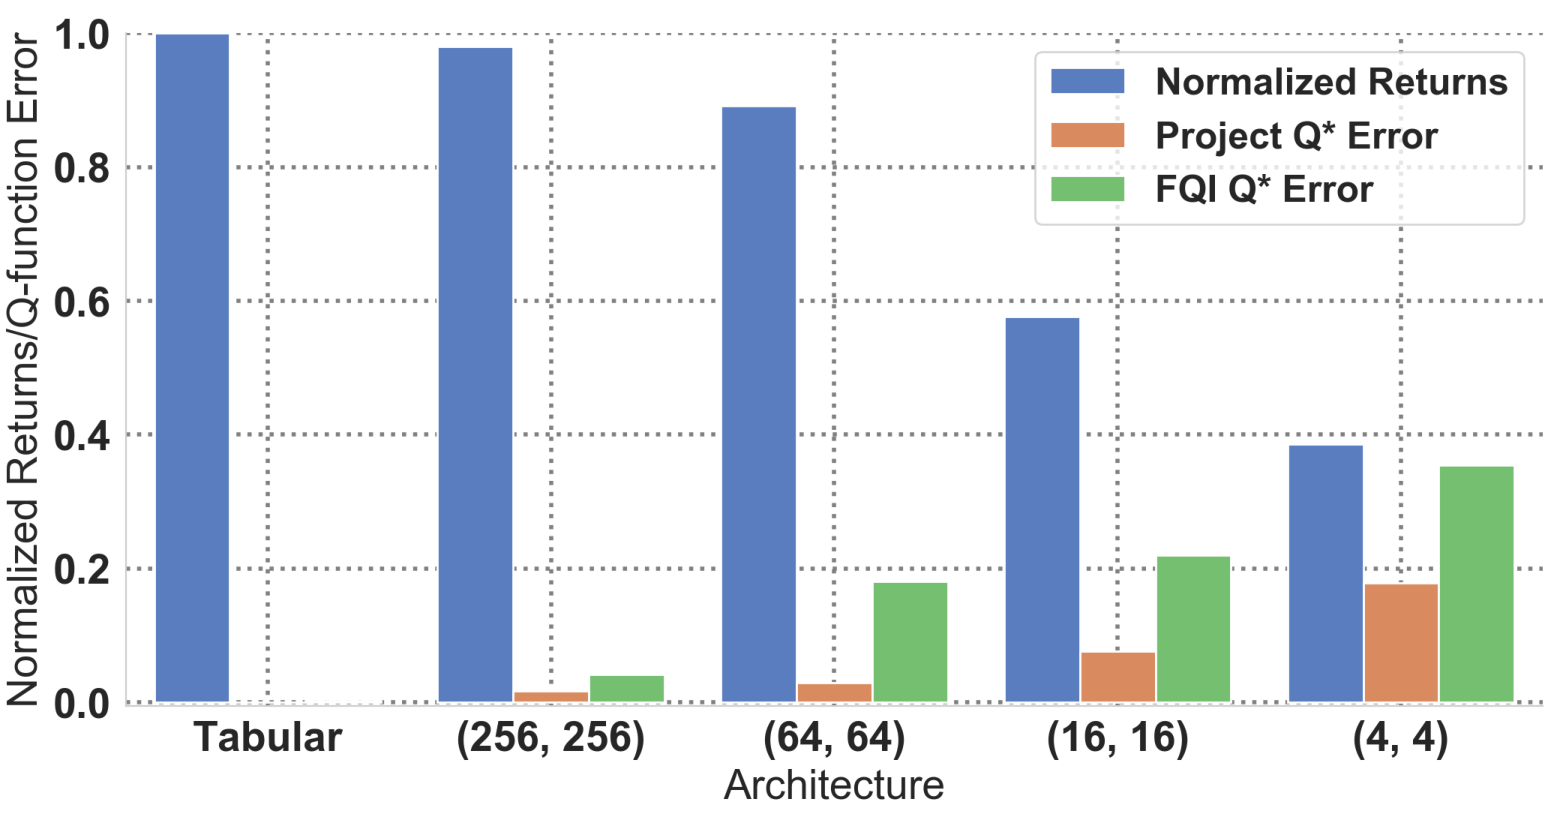
\includegraphics[width=0.7\linewidth]{chapters/diagnosing_q/images/fig_1.pdf}
% generated by plot_doodad_exact_fqi.py:returns_qstar_vs_arch
% data_dir = east1//2019-01-18-newenv-exact-weighting
\vspace{-0.8cm}
\end{figure}

We first note the obvious trend that smaller architectures produce lower returns and converge to worse solutions. 
However, we also find that smaller architectures introduce significant bias in the \textit{learning process}, and there is a significant gap between the solution found by Exact-FQI and the best solution within the model class. 
One explanation is that when the target is bootstrapped, we must represent all Q-functions along the path to the solution, and not only the final result~\citep{Bertsekas96}.
This observation implies that using large architectures is crucial not only because they have capacity to represent a better solution, but also because they are easier to train using bootstrapping. 
We also note that divergence rarely occurs in practice, occuring in only 0.9\% of our experiments (measured as the Q-values growing larger than 10 times $Q^*(s,a)$). 

For high-dimensional problems, we present experiments on varying the architecture of the Q-network in SAC~\cite{Haarnoja18} in Appendix Fig.~\ref{fig:size_sac}. We still observe that large networks have the best performance, and that divergence rarely happens even in high-dimensional continuous spaces. We briefly discuss theoretical intuitions on apparent discrepancy between the lack of unbounded divergence in relation known counterexamples in Appendix~\ref{app:bounded_error}.

\section{Question 2: What is the Impact of Sampling Error and Overfitting?}
\label{sec:overfitting}

%A second source of error in minimizing the Bellman error, orthogonal to function approximation, is that of sampling or generalization error. The next issue we investigate is the effect of sampling error on Q-learning methods.

%\subsection{Technical Background}

Thus far, we have observed that the performance of off-policy RL algorithms based on Q-learning can be quite sensitive to the distribution of the offline dataset, even when all the transition tuples in the MDP are provided to the algorithm and only the weighting over these samples is varied. In this section, we aim to study a distinct question: we study
\begin{wrapfigure}{r}{0.5\linewidth}
    \centering
    \vspace{-10pt}
    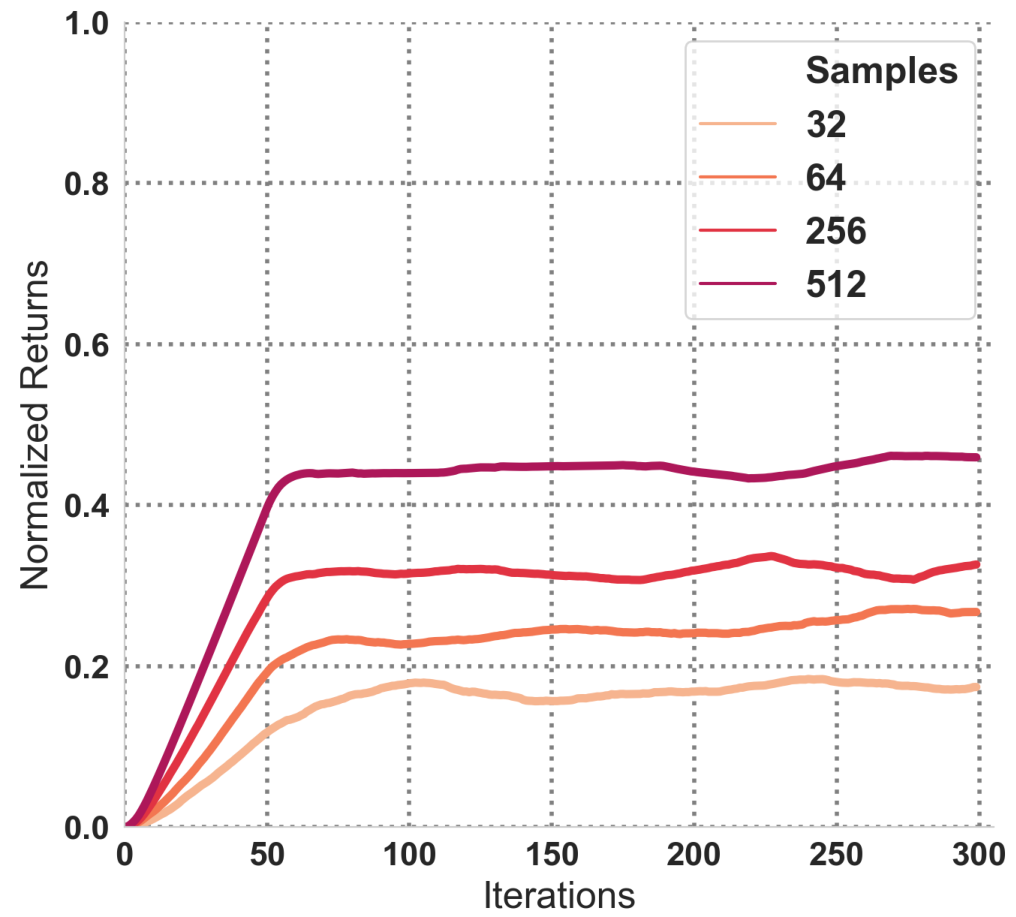
\includegraphics[scale=0.4]{chapters/diagnosing_q/images/samples_arch.pdf}
    \vspace{-0.2cm}
    \caption{\label{fig:sampling_256} Samples plotted with returns for a 256x256 network. More samples yields better performance.}
    \vspace{-0.5cm}
    %plot_sampling
    %east1//2019-01-20-newenv-sample-weighting
\end{wrapfigure}
\!\!the performance of off-policy Q-learning when the offline dataset is of a finite size, and may not contain all transitions in the MDP. To address any confounders from distributional shift, we provide the underlying Q-learning algorithm oracle access to collecting a limited amount of data from the current snapshot of the learned policy. While this sort of active data collection is not possible in the offline RL problem setting, we find that it allows us to more carefully localize the challenges of overfitting and sampling error.

% Approximate dynamic programming assumes that the projection of the Bellman backup (Eqn.~\ref{eqn:bellman_projection}) is computed exactly, but in reinforcement learning we can normally only compute the \textit{empirical Bellman error} over a finite set of samples. In the PAC framework, overfitting can be quantified by a bounded error in between the empirical and expected loss with high probability, which decays with sample size~\citep{Shalev2014}. \citet{munos2008finite, maillard2010finite, tosatto2017boosted} provide such PAC-bounds which account for sampling error in the context of Q-learning and value-based methods, and quantify the quality of the final solution in terms of sample complexity.

We analyze several key points that relate to sampling error. First, we show that Q-learning is prone to overfitting, and that this overfitting has a real impact on performance. 

\subsection{Quantifying Overfitting}
We first quantify the amount of overfitting that happens during training, by varying the number of samples. In order provide comparable validation errors across different experiments, we fix a reference sequence of Q-functions, $Q^1, ... , Q^N$, obtained during an arbitrary run of Q-learning. We then retrace the training sequence, and minimize the projection error $\Projmu(Q^t)$ at each training iteration, using varying amounts of on-policy data or sampling from a replay buffer. We measure the validation error (the expected Bellman error) at each iteration under the on-policy distribution, plotted in Figure~\ref{fig:sampling_validation_loss}. We note the obvious trend that more samples leads to significantly lower validation loss. 
% A more interesting observation is that sampling from the replay buffer results in the lowest on-policy validation loss, despite bias due to distribution mismatch from sampling off-policy data. As we elaborate in Section~\ref{sec:analysis_nonstationarity}, we believe that replay buffers are effective because they reduce overfitting and have good sample coverage over the state space, not necessarily due to reducing the effects of nonstationarity.

Next, Figure~\ref{fig:sampling_256} shows the relationship between number of samples and returns. We see that more samples leads to improved learning speed and a better final solution. A full sweep including architectures is presented in the Appendix (Figure~\ref{fig:sampling_arch_sweep}). Despite overfitting being an issue, larger architectures still perform better because the bias introduced by smaller architectures dominates. This observation indicate that the nature of overfitting in RL is likely significantly different from that of supervised learning: while overfitting in supervised learning can bne controlled by regulating model capacity, off-policy RL methods likely need to rely on alternative techniques to control overfitting. We have made some progress towards understanding this questions in \citet{li2022effective}.   

\begin{figure*}[ttt!]
\begin{subfigure}{0.31\linewidth}
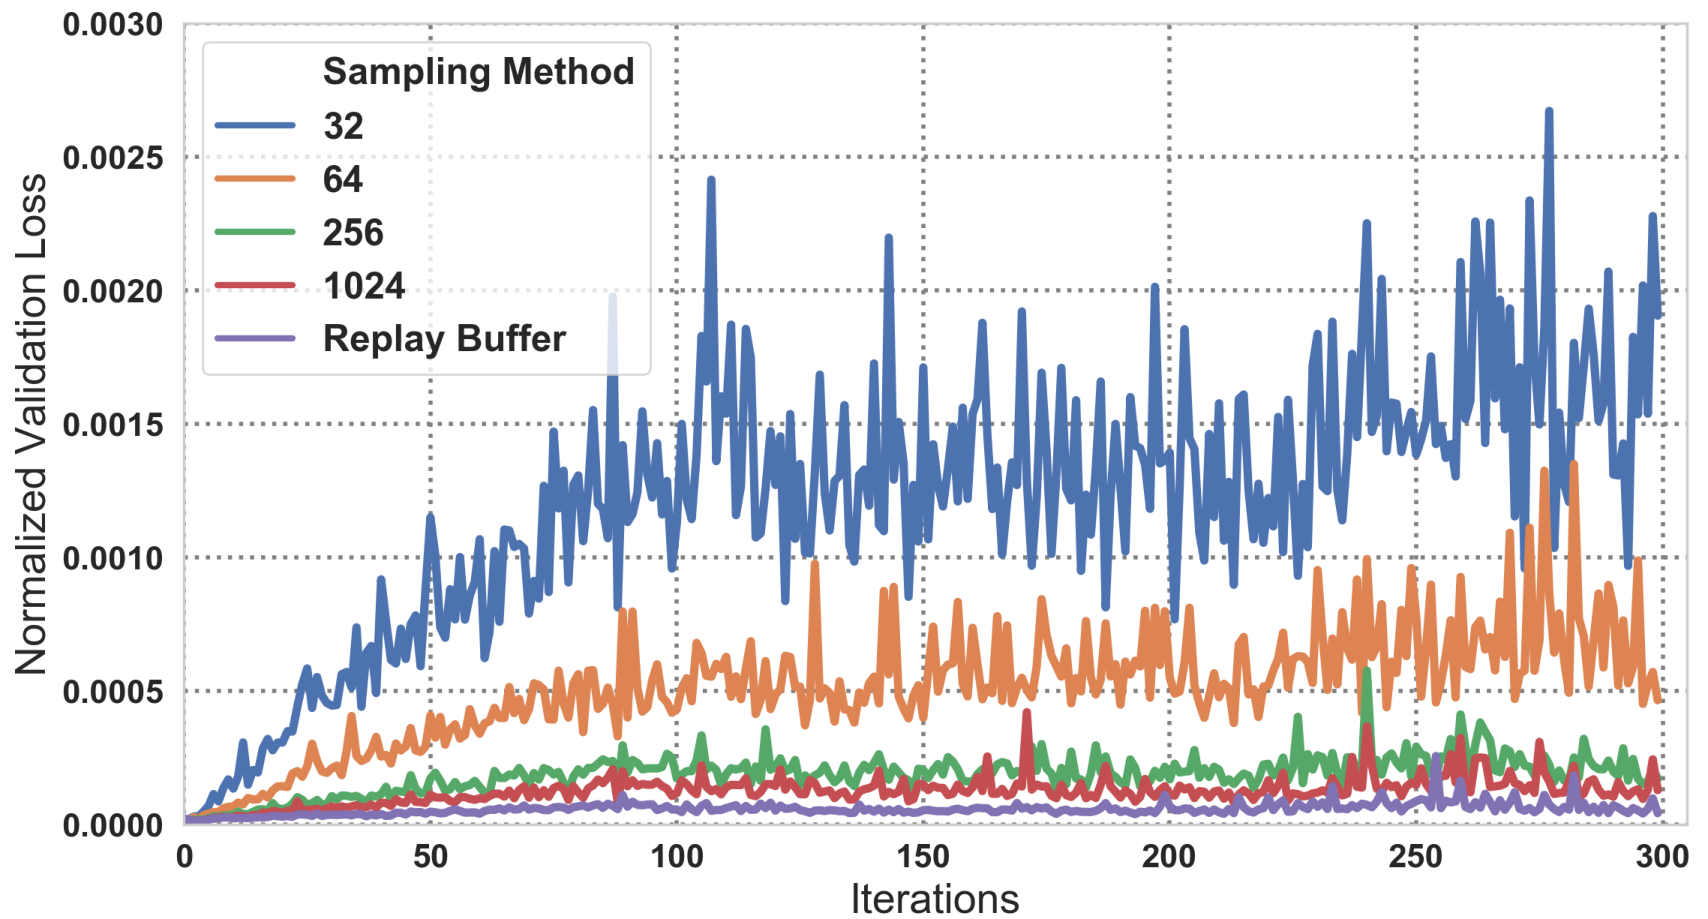
\includegraphics[width=0.97\linewidth]{chapters/diagnosing_q/images/overfitting.pdf}
%plot_overfitting
%central1//2019-01-21-overfitting-coupled
\caption{\label{fig:sampling_validation_loss} On-policy validation losses for varying amounts of on-policy data (or replay buffer), averaged across environments and seeds. Note that sampling from the replay buffer has lower on-policy validation loss, despite bias from distribution shift.}
\end{subfigure}
~\vline~
\begin{subfigure}{0.31\linewidth}
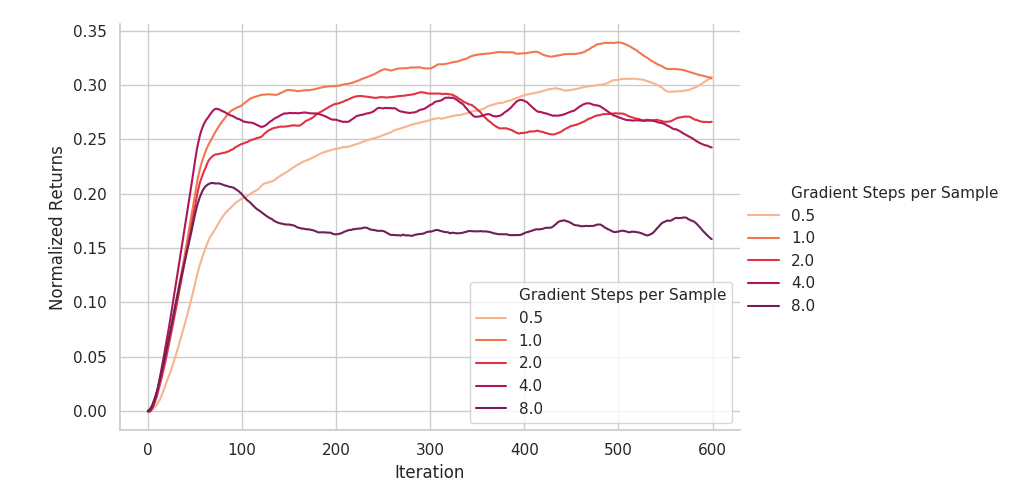
\includegraphics[trim={0 0 7.0cm 0},clip,width=0.97\linewidth]{chapters/diagnosing_q/images/grad_steps_fqi}
%plot_overfitting
%central1//2019-01-21-overfitting-coupled
\caption{\label{fig:fqi_grad_sweep}Normalized returns plotted over training iterations (32 samples per iteration), for different ratios of gradient steps per sample. We observe that intermediate values of gradient steps work best, and too many gradient steps hurt performance.}
\end{subfigure}
~\vline~
\begin{subfigure}{0.31\linewidth}
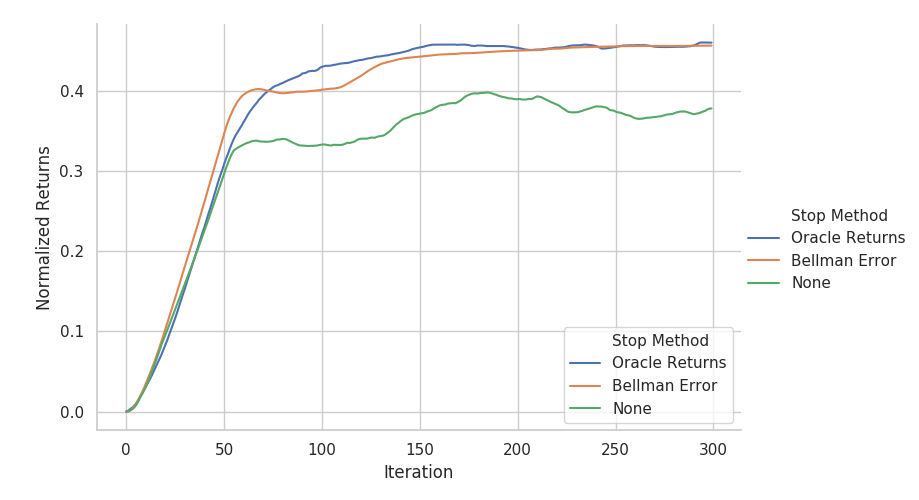
\includegraphics[trim={0 0 4.4cm 0},clip,width=0.97\linewidth]{chapters/diagnosing_q/images/validation_stop}
%plot_validation_stop
%west1//2019-02-20-replay-validation-stop
\caption{\label{fig:validation_stop}Normalized returns plotted over training iterations (32 samples are taken per iteration), for different early stopping methods. We observe that using proper early stopping can result in a modest performance increase.}
\end{subfigure}
\end{figure*}

\subsection{Does Compensating for Overfitting Improve Performance?}

Finally, to confirm our hypotheses regarding overfitting, we now wish to understand if compensating for overfitting does lead to improved performance. One common technique for reducing overfitting is to utilize \textit{early stopping} methods to mitigate overfitting without reducing model size.
% We first note that the number of gradient steps taken per sample in the projection step has an important effect on performance -- too few steps and the algorithm learns slowly, but too many steps and the algorithm may initially learn quickly but overfit. To show this, we run an ablation over the number of gradient steps taken per sample in Replay-FQI and TD3 (TD3 uses 1 by default). Results for FQI are shown in Fig.~\ref{fig:fqi_grad_sweep}, and for TD3 in Appendix Fig.~\ref{fig:td3_grad_sweep}.
In order to understand whether early stopping criteria can reduce overfitting, we employ \emph{oracle} stopping rules to provide an ``upper bound'' on the best potential improvement. We try two criteria for setting the number of gradient steps: the expected Bellman error and the expected returns of the greedy policy (oracle returns). We implement both methods by minimizing the TD-error to convergence, and retroactively selecting the intermediate Q-function which is judged best by the evaluation metric. Using oracle stopping metrics results in a modest boost in performance in tabular domains (Fig.~\ref{fig:validation_stop}). Thus, we believe that there is promise in further improving such early-stopping methods for reducing overfitting in deep RL algorithms.

~

\textbf{To summarize}, we can draw a few conclusions from our experiments in this section. First, overfitting is indeed an issue with Q-learning, and too many gradient steps or too few samples can lead to poor performance. Second, although overfitting is a problem, large architectures are still preferred, because the bias from function approximation outweighs the increased overfitting from using large models. 

Finally, we also remark that attempting to learn optimal policies from a static offline dataset will present both distributional shift and overfitting challenges together, and we would expect these to be tightly coupled with each other in the following sense: the inability to correclty identify the underlying MDP from finite samples in the offline dataset will induce errors in policy optimization, and these errors would then be exacerbated in the next step of learning as the learned policy deviates from the training data. This will also be evident in the theoretical results that we will present in subsequent chapters.    
\section{Non-Stationarity}
\label{sec:analysis_nonstationarity}

%In this section, we discuss issues related to the non-stationarity of the Q-learning process (relating to the Bellman backup and Bellman error minimization).

%\subsection{Technical Background}
Instability in Q-learning methods is often attributed to the nonstationarity of the objective \citep{Lillicrap2015,Mnih2015}. 
Nonstationarity occurs in two places: in the changing target values $\backup Q$, and in a changing weighting distribution $\mu$ (``distribution shift''). 
Note that a non-stationary objective, by itself, is not indicative of instability. For example, gradient descent can be viewed as successively minimizing linear approximations to a function: for gradient descent on $f$ with parameter $\theta$ and learning rate $\alpha$, we have the ``moving'' objective $\theta^{t+1} = \argmin{\theta}\{ \theta^T \nabla_\theta f(\theta^t) - \frac{1}{2\alpha} \normtt{\theta - \theta^t} \} = \theta^t - \alpha \nabla_\theta f(\theta^t)$. 
However, the fact that the Q-learning algorithm prescribes an update rule and not a stationary objective complicates analysis. Indeed, the motivation behind algorithms such as GTD~\citep{Sutton09a, Sutton09b}, approximate linear programming~\citep{de2002alp}, and residual methods~\citep{Baird1995,scherrer2010residual} can be seen as introducing a stationary objective that can be optimized with standard methods such as gradient descent.
%Therefore, a key question to investigate is whether these non-stationarities are detrimental to the learning process.
% \vspace{-25pt}

\subsection{Does a moving target cause instability in the absence of a moving distribution?}

To study the moving target problem, we first isolate the speed at which the target changes. To this end, we define the $\alpha$-smoothed Bellman backup, $\backup^\alpha$, which computes an exponentially smoothed update as follows: 
$\backup^{\alpha}Q = \alpha \backup Q + (1-\alpha)Q$.
% \vspace{-5pt}
This scheme is inspired by the soft target update used in algorithms such as DDPG~\citep{Lillicrap2015} and SAC~\citep{Haarnoja2017} to improve the stability of learning. Standard Q-iteration uses a ``hard'' update where $\alpha=1$. A soft target update weakens the contraction of Q-iteration from $\gamma$ to $1-\alpha+\alpha\gamma$ (see Appendix~\ref{app:alpha_smoothed_q}),
so we expect slower convergence, but perhaps it is more stable under heavy function approximation error. We performed experiments with this modified backup using Exact-FQI under the $\text{Unif}(s,a)$ weighting distribution.

Our results are presented in Appendix Fig.~\ref{fig:smooth_fqi}.
We find that the most cases, the hard update with $\alpha=1$ results in the fastest convergence and highest asymptotic performance. However, for smaller architectures, $4 \times 4$ and $16 \times 16$, lower values of $\alpha$ (such as 0.1) achieve slightly higher asymptotic performance. Thus, while more expressive architectures are still stable under fast-changing targets, we believe that a slowly moving target may have benefits under heavy approximation error. This evidence points to either using large function approximators, in line with the conclusions drawn in the previous sections, or slowing the target updates on problems with high approximation error.

\subsection{Does distribution shift impact performance?}
\label{sec:distr_shift}

\begin{figure}[tb]
\caption{\label{fig:distribution_shift_tv_loss} Distribution shift and loss shift plotted against time. Prioritized and on-policy distributions induce the greatest shift, whereas replay buffers greatly reduce the amount of shift.}
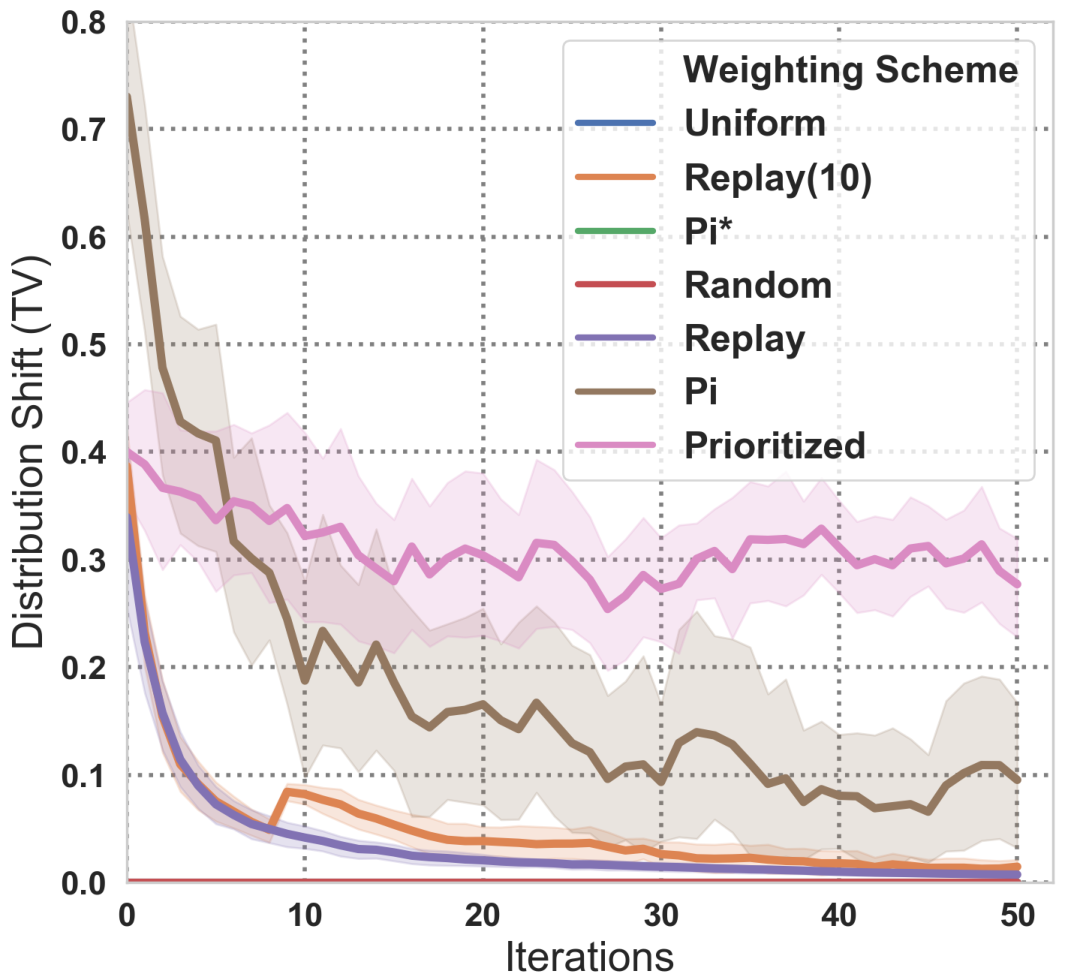
\includegraphics[width=0.51\columnwidth]{chapters/diagnosing_q/images/dist_shift_tv3.pdf}
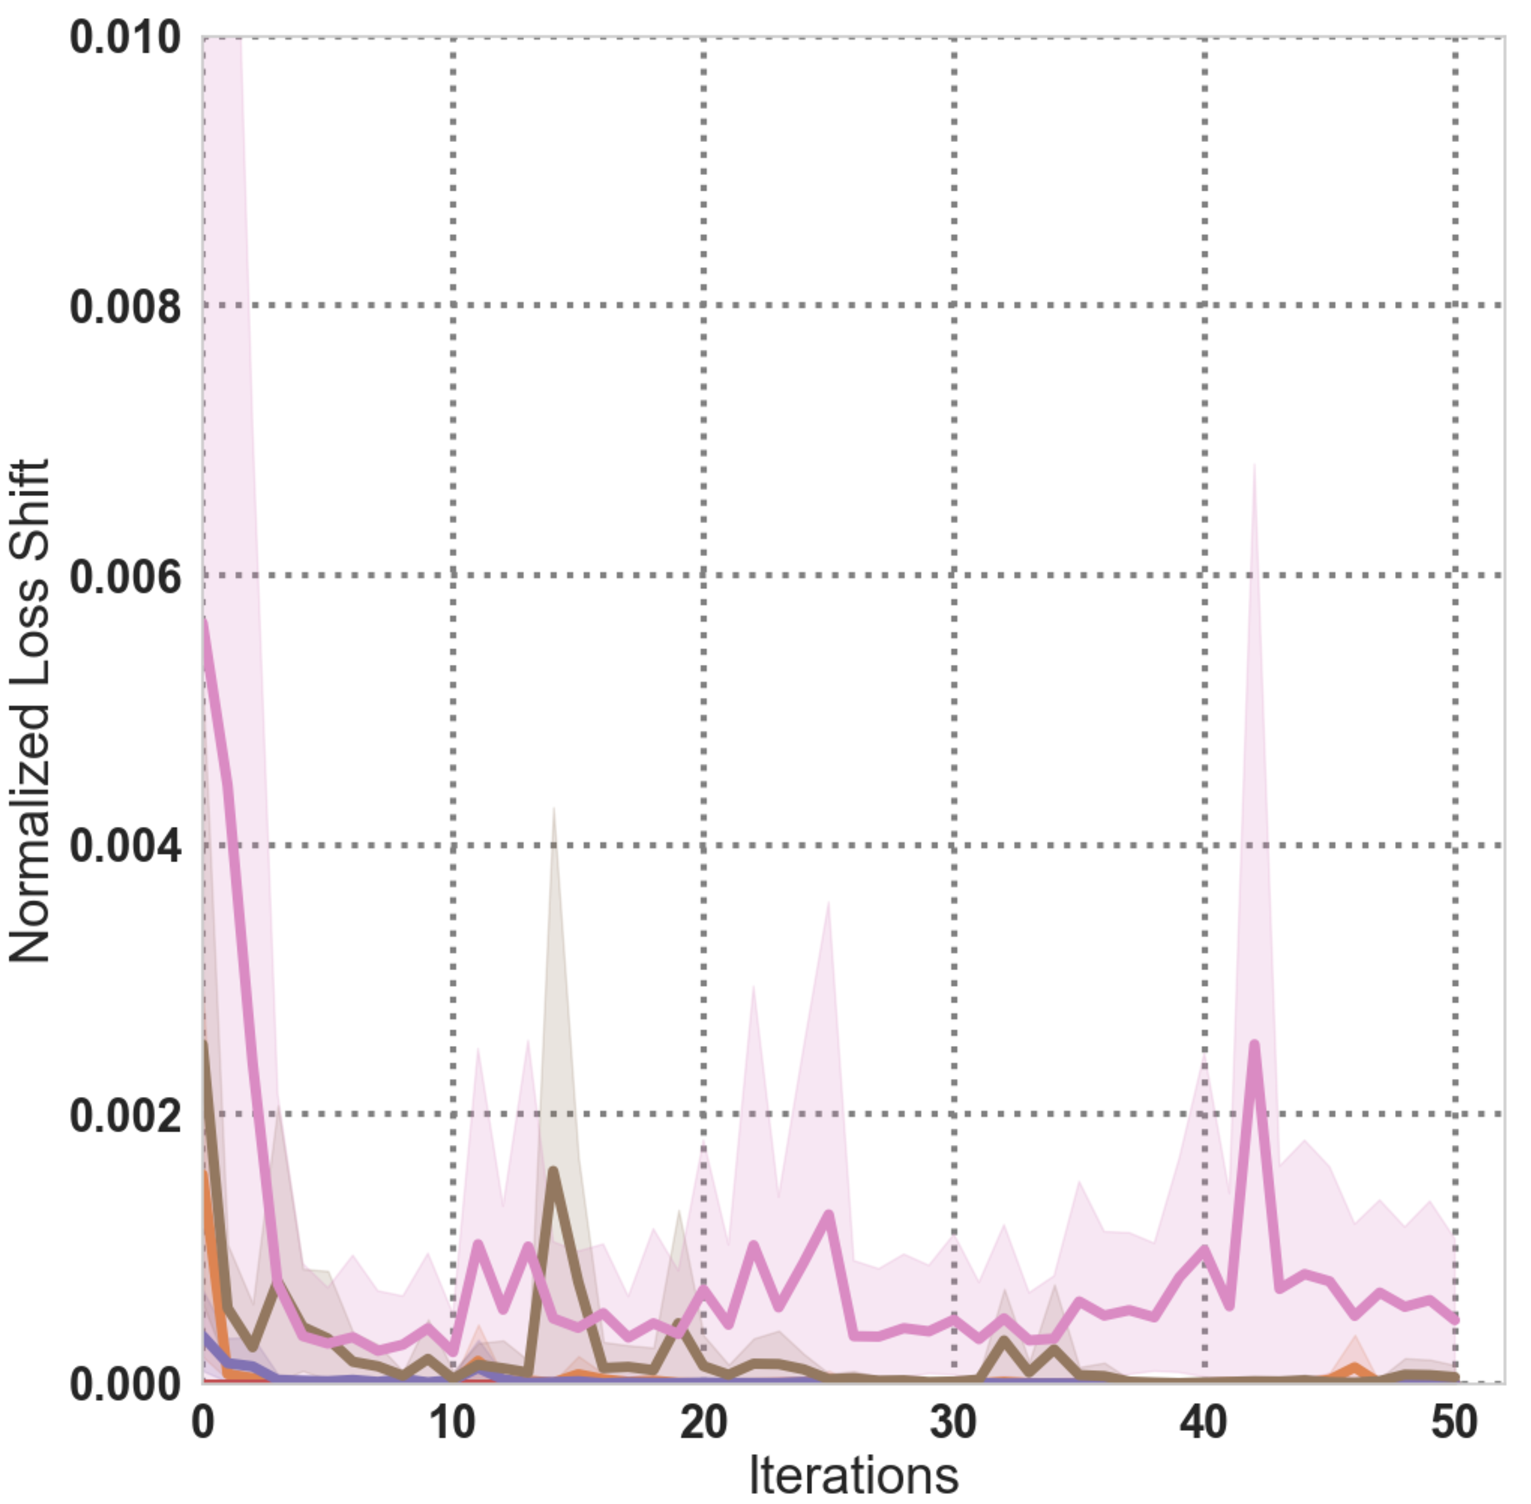
\includegraphics[width=0.47\columnwidth]{chapters/diagnosing_q/images/dist_shift_loss_tv3.pdf}
% \vspace{-10pt}
% generated by plot_distribution_shift.py:plot_tv_loss_over_time
% data_dir = east1//2019-01-18-newenv-exact-weighting
\end{figure}


To study the distribution shift problem, we exactly compute the amount of distribution shift between iterations in total-variation distance, $D_{TV}(\mu^{t+1} || \mu^{t})$ and the ``loss shift'':
$\mathbb{E}_{\mu^{t+1}}[ (Q^{t} - \backup Q^{t})^2] - \mathbb{E}_{\mu^{t}}[ (Q^{t} - \backup Q^{t})^2]$.
The loss shift quantifies the Bellman error objective when evaluated under a new distribution - if the distribution shifts to previously unseen states, we would expect a highly inaccurate Q-value in such states, leading to high loss shift.

% \begin{figure}[ht]

% \end{figure}


We run our experiments using Exact-FQI with a 256x256 layer architecture, and plot the distribution discrepancy and the loss discrepancy in Fig.~\ref{fig:distribution_shift_tv_loss}. 
We find that Prioritized$(s,a)$ has the greatest shift, followed by on-policy variants. Replay buffers greatly reduce distribution shift compared to on-policy learning, which is similar to the de-correlation argument cited for its use by~\citet{Mnih2015}.
However, we find that this metric correlates little with the performance of FQI (Fig.~\ref{fig:distribution_shift_vs_returns}). For example, prioritized weighting performs well yet has high distribution shift.

Overall, our experiments indicate that nonstationarities in both distributions and target values, when isolated, do not cause significant stability issues. Instead, other factors such as sampling error and function approximation appear to have more significant effects on performance.
%Therefore, we investigate how to design a \emph{better} sampling distribution, without regard to nonstationarity, in the next section.
%In the light of these findings, we might therefore ask: can we design a \emph{better} sampling distribution, without regard for distributional shift and with regard for high-entropy, that results in better final performance, and is realizable in practice? We investigate this in the following section.

\vspace{-0.2cm}
\section{Impact of Distributional Shift}
\label{sec:sampling_distributions}
\vspace{-0.2cm}

%As alluded to in Section~\ref{sec:analysis_nonstationarity}, the choice of sampling distribution $\mu$ is an important design decision can have a large impact on performance. Indeed, it is not immediately clear which distribution is ideal for Q-learning. In this section, we hope to shed some light on this issue.

%\subsection{Technical Background}
% Off-policy data has been cited as one of the ``deadly triads'' for Q-learning~\citep{suttonrlbook}, which has potential to cause instabilities in learning. On-policy distributions~\citep{Tsitsiklis1997} and fixed behavior distributions~\citep{Sutton09a,Maei2010} have often been targeted for theoretical convergence analysis, and many works use importance sampling to correct for off-policyness~\citep{precup2001offpol, munos2016safe}
% However, to our knowledge, there is relatively little guidance which compares how different weighting distributions compare in terms of convergence rate and final solutions.

% Off-policy RL methods applied to the offline RL problem would typically attempt to learn an optimal policy, even though the static dataset may not be generated from an optimal policy. As a result, one issue to emerge is that of \emph{distributional shift}: while these methods can only train a model of the value-function and the policy using state-action tuples from the data, these models  will need to make correct predictions on states and actions sampled from a different distribution encountered upon deployment. In general, models trained via machine learning are not robust when the distribution of inputs changes, indicating that distributional shift can be challenge for off-policy RL methods. Is distributional shift a challenge in offline RL?   

Off-policy RL methods applied to the offline RL problem would typically attempt to learn an optimal policy, even though the static dataset may not be generated from an optimal policy. As a result, one issue that emerges is that of \emph{distributional shift}: while these methods train a model of the value-function and the policy only using state-action tuples from the data, upon deployment, these models will need to make correct predictions on states and actions sampled from a different distribution of the learned policy. In general, models trained via machine learning are not robust when the distribution of inputs changes, indicating that distributional shift can be a challenge for off-policy RL methods. Is distributional shift a challenge in offline RL?

Indeed, theoretically, the effects of distributional shift have been quantified using the notion of a concentrability coefficient~\citep{munos2005erroravi}, a constant typically $\gg 1$, which provides a worst-case error bound on the performance of an off-policy RL method due to distributional shift. To evaluate if this challenge persists empirically as well, we will analyze Q-learning methods for various choices of data distributions in this section.

A crucial design decision we must make is to consider setups that do not confound distributional shift with access to limited data. Therefore, for our study, we provide the underlying algorithm oracle access to all state-action transitions in the MDP, but vary the \emph{distribution} over state-action pairs from which these transitions are sampled.

% Indeed, theoretically, the effects of distributional shift have been quantified using the notion of a concentrability coefficient~\citep{munos2005erroravi}, a constant typically $\ggt 1$, which provides a worst-case error bound on the performance of an off-policy RL method due to distributional shift. To evaluate if this challenge persists empirically as well, we will analyze Q-learning methods for various choices of data distributions in this section. 

% A crucial design decision we must make is to consider setups that do not confound distributional shift with access to limited data. Therefore, for our study, we provide the underlying algorithm oracle access to all state-action transitions in the MDP, but vary the \emph{distribution} over state-action pairs that these transitions are sampled according to.   
% ~\citep{NIPS2017_6913} suggests that when the state-distribution is fixed, the action distribution should be weighted by the optimal policy for residual Bellman errors. In deep RL, prioritized replay~\citep{Schaul2015}, and mixing replay buffer with on-policy data~\citep{hausknecht2016policy,zhang2018deeper} have been found to be effective. %We aim to empirically analyze multiple choices for weighting distributions to determine which are the most effective.

%\vspace{-10pt}
\vspace{-0.2cm}
\subsection{What Are the Best Data Distributions Without Sampling Error?}
\label{subsec:dist_shift_exact}
\vspace{-0.2cm}

% \begin{figure*}[ttt!]
% \begin{subfigure}{0.3\linewidth}
% \caption{\footnotesize \label{fig:distribution_shift_vs_returns} Average distribution shift across time for different data distributions, plotted against returns for a 256x256 model. We find that distribution shift does not have strong correlation with returns.}
% 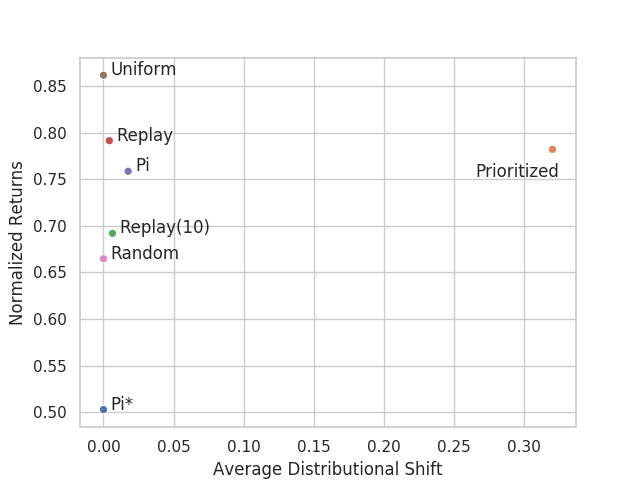
\includegraphics[width=0.99\columnwidth]{chapters/diagnosing_q/images/returns_vs_shift}
% % generated by plot_distribution_shift.py
% % data_dir = east1//2019-02-12-exact-weighting-distr-shift
% \vspace{-0.2in}
% \end{subfigure}
% ~\vline~
% \begin{subfigure}{0.3\linewidth}
% \caption{\footnotesize \label{fig:weighting_schemes} Weighting distribution versus architecture in Exact-FQI. Replay(s, a) consistently provides the highest performance. Note that Adversarial Feature Matching is comparable to Replay(s, a), but surprisingly better for small networks. }
% 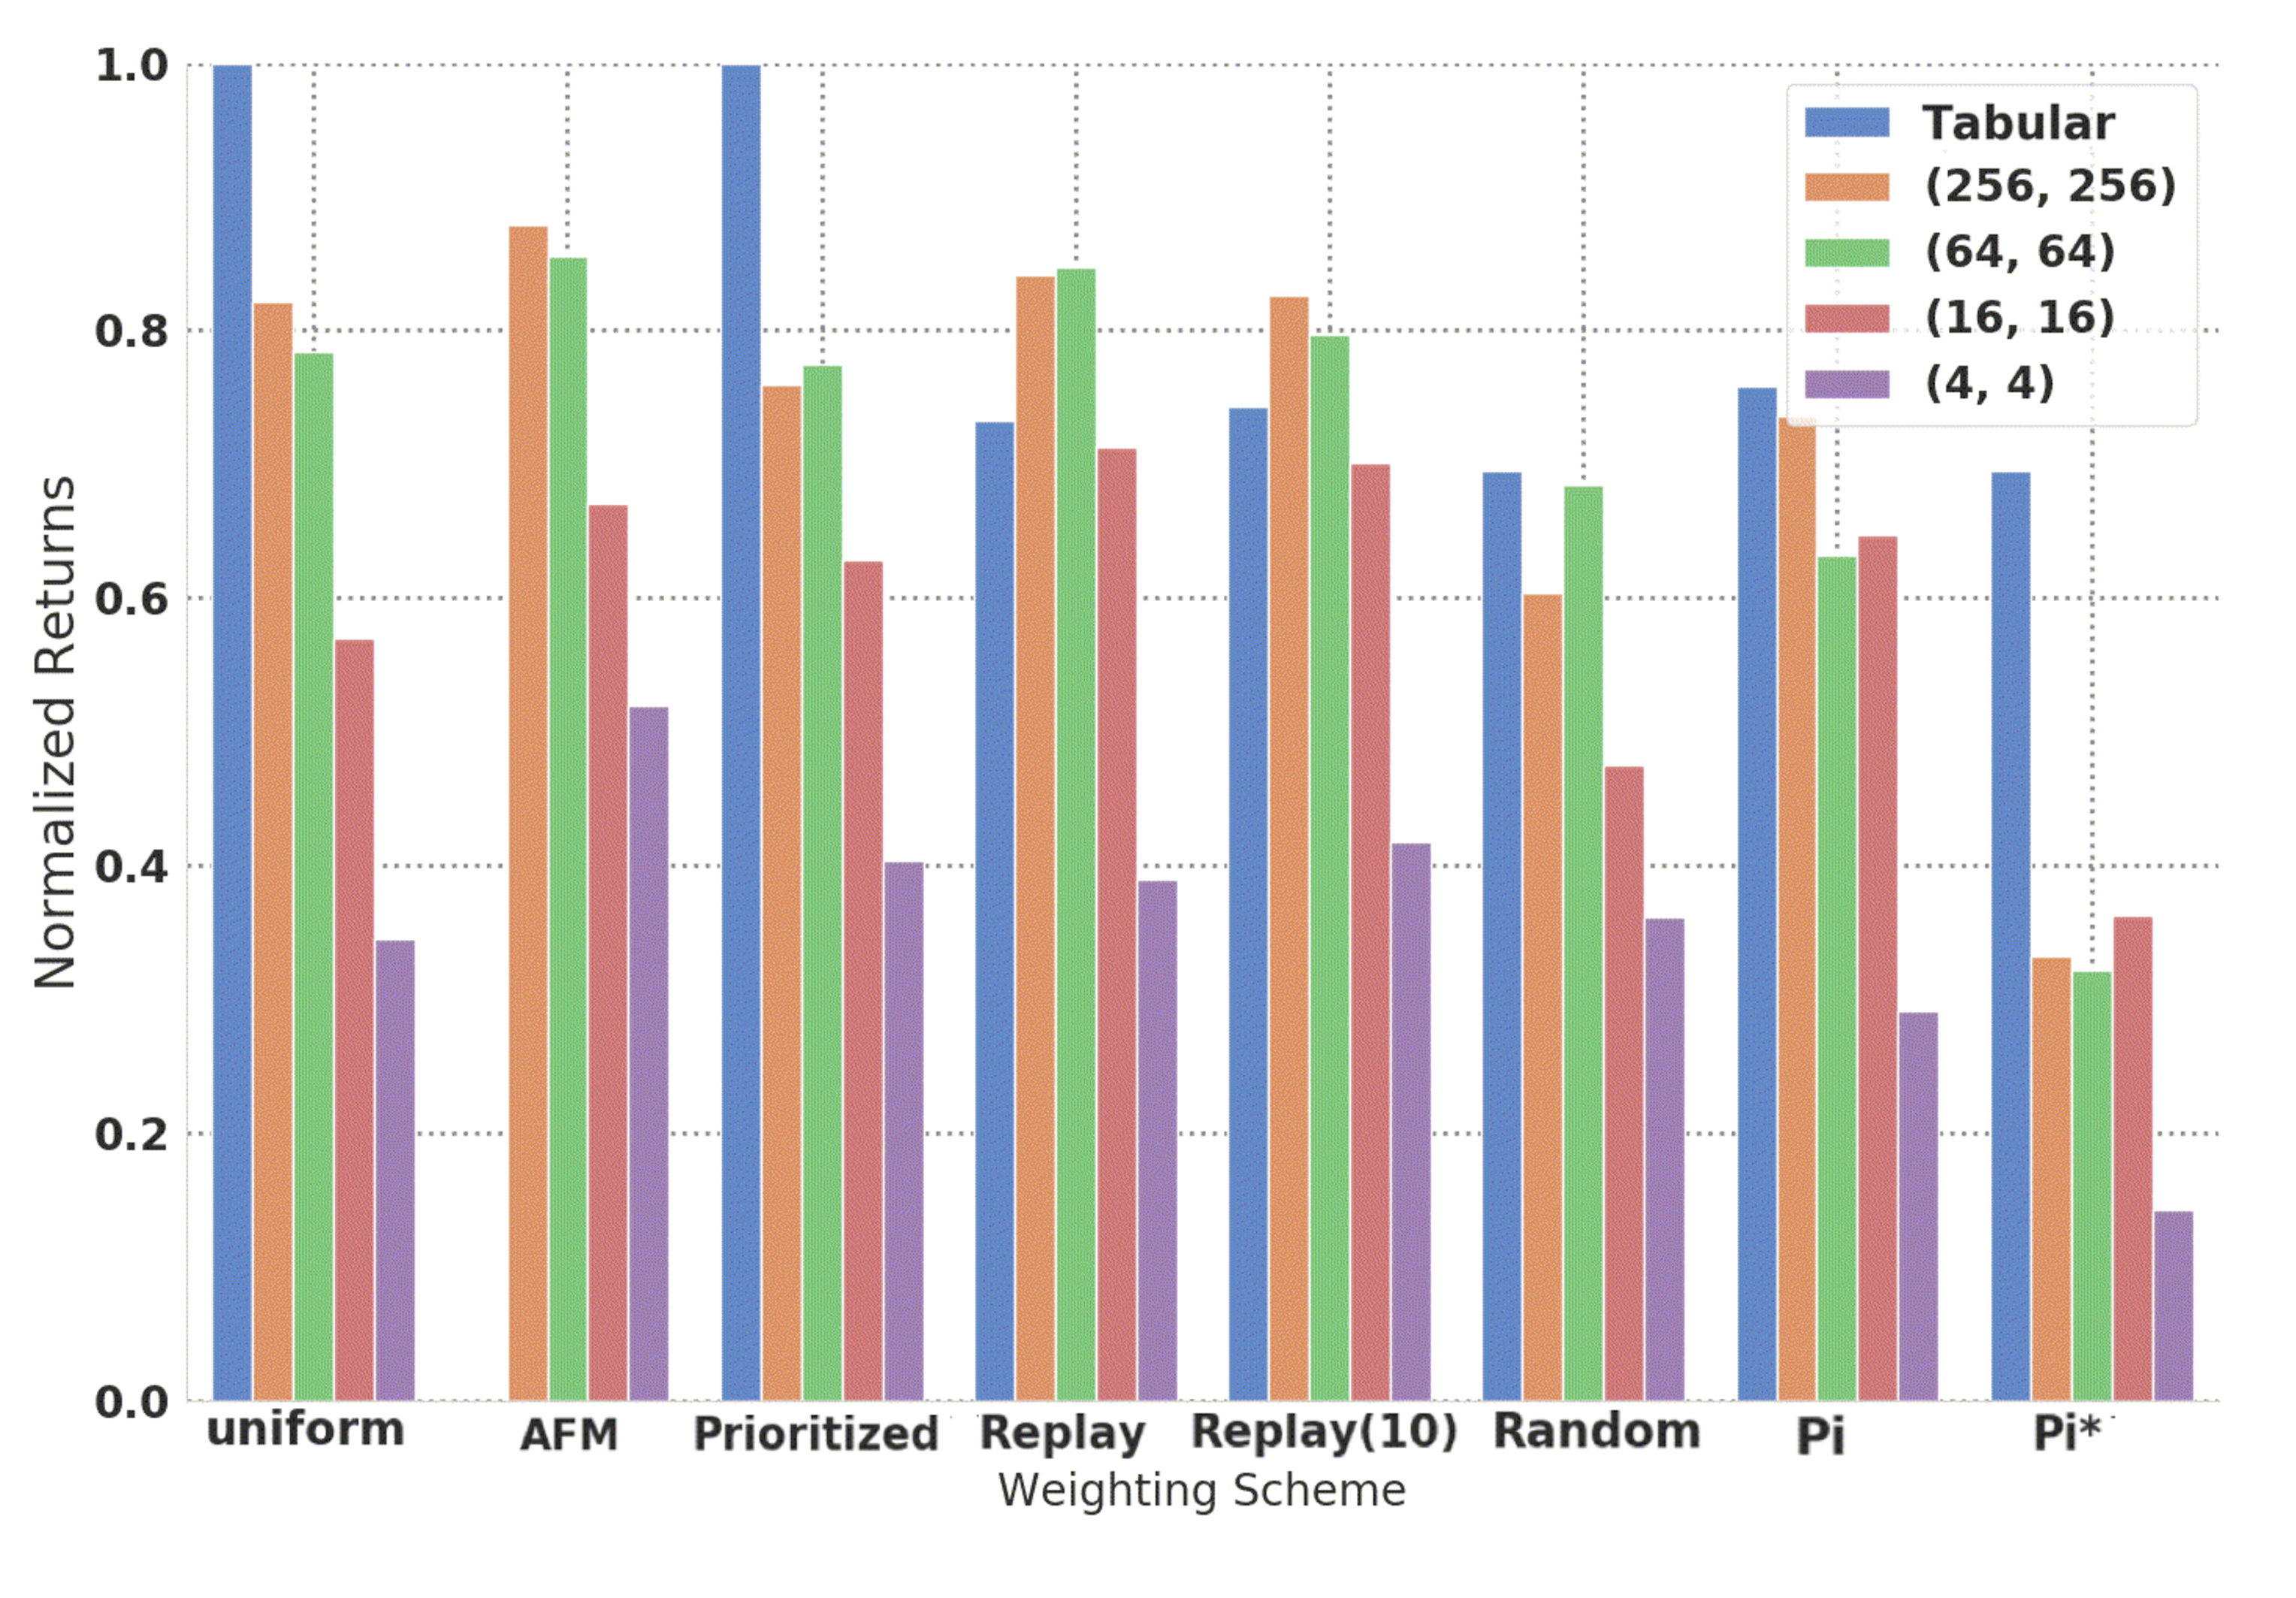
\includegraphics[width=0.99\columnwidth]{chapters/diagnosing_q/images/exact_fqi_schemes.pdf}
% % generated by plot_exact_weighting.py
% % data_dir = east1//2019-01-18-newenv-exact-weighting
% \vspace{-0.3in}
% \end{subfigure}
% ~\vline~
% \begin{subfigure}{0.3\linewidth}
% \caption{\footnotesize \label{fig:weighting_entropy_vs_returns} Normalized returns plotted against normalized entropy for different weighting distributions. All experiments use Exact-FQI with a 256x256 network. We see a general trend that high-entropy distributions lead to greater performance.}
% 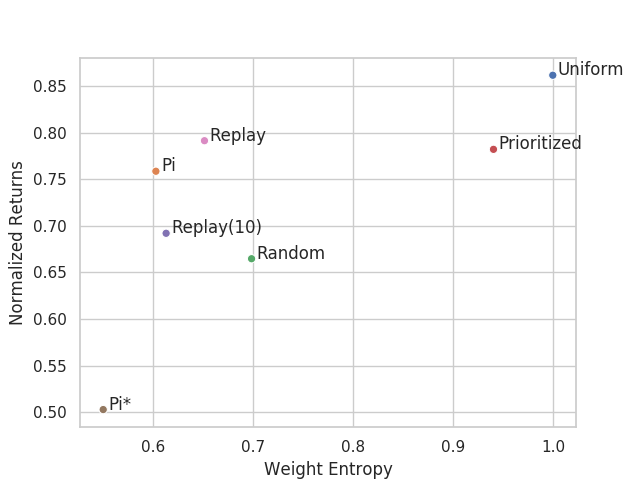
\includegraphics[width=0.99\columnwidth]{chapters/diagnosing_q/images/returns_vs_entropy}
% % generated by plot_distribution_shift.py
% % data_dir = east1//2019-02-12-exact-weighting-distr-shift
% \end{subfigure}
% \end{figure*}

\begin{wrapfigure}{r}{0.45\linewidth}
    \vspace{-0.2cm}
    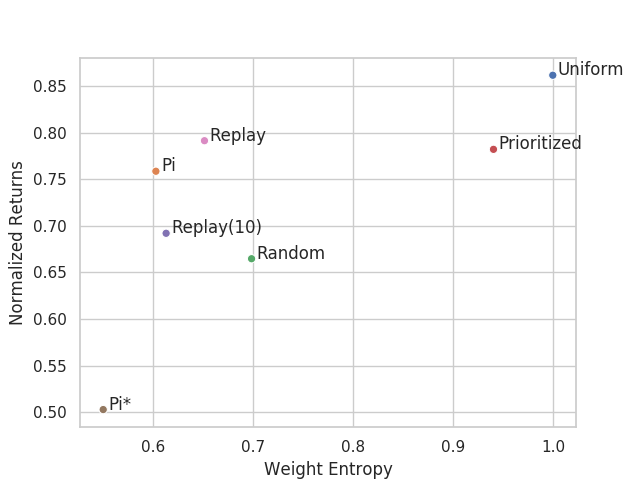
\includegraphics[width=0.99\linewidth]{chapters/diagnosing_q/images/returns_vs_entropy}
    \caption{\footnotesize \label{fig:weighting_entropy_vs_returns} Normalized returns plotted against normalized entropy for different weighting distributions. All experiments assume access to all state-action pairs with a 256x256 Q-network. We see a general trend that high-entropy distributions lead to greater performance, corroborating the uniformity hypothesis.}
    \vspace{-0.2cm}
    % generated by plot_distribution_shift.py
    % data_dir = east1//2019-02-12-exact-weighting-distr-shift
\end{wrapfigure}
We begin by studying the effect of data distributions when disentangled from sampling error. We run Q-learning with an ablation over various Q-function network architectures and data distributions and report our aggregate results in Fig.~\ref{fig:weighting_entropy_vs_returns}. $\text{Unif}(\bs, \mathbf{a})$, $\text{Replay}(\bs, \mathbf{a})$ (using a replay buffer consisting of data from a mixture of policies with different degrees of optimality), and $\text{Prioritized}(\bs, \mathbf{a})$ (weighting induced by prioritized experience replay~\citep{Schaul2015}) consistently result in the highest returns across all architectures. On the other hand, relatively ``narrow'' data distributions, such as those induced the optimal policy ($\pi^*$) or only using a mixture of a few policies ($\text{Replay}(10)$) results in poor performance.
% We believe that these results are in favor of the \textit{uniformity} hypothesis: intuitively, the best distributions spread weight across larger support of the state-action space, reducing the amount of possible distributional shift. On the other hand, less-uniform distributions such as the state-action distirbution induced by the optimal policy, present multiple avenues to deviate away from the offline data distribution, resulting in larger distributional shift.
We believe that these results favor the \textit{uniformity} hypothesis: intuitively, the best distributions spread weight across a larger support of the state-action space, reducing the amount of possible distributional shift. On the other hand, less-uniform distributions, such as the state-action distribution induced by the optimal policy, present multiple avenues to deviate away from the offline data distribution, resulting in larger distributional shift.

\textbf{To summarize}, this indicates that narrow data distributions lead to worse performance compared to higher-entropy data distributions, indicating that distributional shift can have a significant impact on the performance of off-policy RL in the offline setting.
%These distributions generally result in the tightest contraction rates, and allow the Q-function to focus on high-error regions. 
%In the sampled setting, this observation motivates exploration algorithms that maximize state coverage (for example, ~\citet{hazan2018} solve an exploration objective which maximizes state-space entropy).
%However, note that in this particular experiment is distinct from exploration, as there is no sampling involved. 
%All states are observed, just with different weights, thus isolating the issue of distributions from the issue of sampling.
\documentclass[../thesis.tex]{subfiles}
\begin{document}
In this thesis, we have presented a number of advances towards learning based 3D object reconstruction. In Chapter \ref{chapter:CategoryShapes}, we presented an algorithm to learn category-specific deformable 3D models for diverse object categories and showed how to use them in conjunction with recognition systems to achieve fully automatic object localization and reconstruction from a single image. In Chapter \ref{chapter:Amodal}, we worked towards calibrating the size of the reconstructed objects by inferring their relative sizes and depths from a single image. We did this by leveraging amodal bounding boxes and reasoning about object co-occurences in image collections. We worked towards unifying single and multi-view reconstruction with a CNN in Chapter \ref{chapter:LSM} with Learnt Stereo Machines.

We have still just scratched the tip of the iceberg as alluded to in the limitations of current works in the chapters above. A number of challenges remain in tightly integrating semantic reasoning and 3D reconstruction (some of which we summarize below) and present for exciting directions for future work. 

\paragraph{Shape Representations:} In our works, we have explored using deformable meshes, voxel occupancy grids and depth maps as representations for shape. While each presents its own benefits, it is still unclear whether one has all the desirable properties for shape representations. For example, part compositionality plays a crucial role in the human visual system which none of the above representations exhibit. There have been promising works towards modelling shapes with primitives such as planes and simple shapes~\cite{abstractionTulsiani17} (cubes, cylinders \etc). Automatic discovery of such primitives which can be shared across object categories would allow for greater interpretability in reconstructions.

\paragraph{Learning without explicit supervision:} We, as humans, almost never have ``ground truth'' data to learn from - especially for 3D shapes. Our mental models are built from observing objects from different viewpoints, in various lighting conditions, by interacting with them \etc This remains a critical problem to solve for current learning systems to scale beyond available 3D datasets. Some recent works~\cite{tulsiani2017multi,zhou2017unsupervised} have investigated using motion and projection into novel views as a proxy for learning shapes. An exciting direction to investigate would be coupling active exploration with 3D shape inference. For example, a robot could derive shape cues for an object by trying to grasp/poke/manipulate it in certain ways.

\paragraph{Quality of reconstructions:} A common issue with current methods for learning-based shape inference methods is that they dont produce high quality outputs (in terms of accuracy, fidelity and resolution). This is in contrast with classical systems which produce extremely detailed models, albeit from far more images. Recent attempts at modelling high resolution grids with CNNs~\cite{hane2017hierarchical} present a promising direction towards detailed reconstructions with learning-based cues. A related task is modelling large spaces with such systems which couples with the question of what shape representations are amenable to such problems.

\paragraph{Related tasks:} While inferring 3D shape from 2D views is an end in itself, it can be especially useful for a number of complementary and upstream tasks. For example, estimating lighting and reflectance in scenes could benefit from learning-based 3D inference systems, particularly when learnt jointly~\cite{barronPAMI13}. More examples of properties for which are difficult to \textit{ground-truth} and tightly coupled with 3D reasoning are optical flow and scene flow. Learning systems could provide a very natural way of jointly modelling these variety of tasks with strong inter-dependencies. Implicit 3D reasoning could also play a critical role in end-to-end learning of policies in robotics~\cite{finn2016end}, \eg for navigating in 3D scenes or manipulating objects.

\end{document}

% Acknowledgements should only appear in the accepted version.
%\section*{Acknowledgements}

%\textbf{Do not} include acknowledgements in the initial version of
%the paper submitted for blind review.

%If a paper is accepted, the final camera-ready version can (and
%probably should) include acknowledgements. In this case, please
%place such acknowledgements in an unnumbered section at the
%end of the paper. Typically, this will include thanks to reviewers
%who gave useful comments, to colleagues who contributed to the ideas,
%and to funding agencies and corporate sponsors that provided financial
%support.
%\clearpage
\bibliography{example_paper}
\bibliographystyle{icml2019}


%%%%%%%%%%%%%%%%%%%%%%%%%%%%%%%%%%%%%%%%%%%%%%%%%%%%%%%%%%%%%%%%%%%%%%%%%%%%%%%
%%%%%%%%%%%%%%%%%%%%%%%%%%%%%%%%%%%%%%%%%%%%%%%%%%%%%%%%%%%%%%%%%%%%%%%%%%%%%%%
% DELETE THIS PART. DO NOT PLACE CONTENT AFTER THE REFERENCES!
%%%%%%%%%%%%%%%%%%%%%%%%%%%%%%%%%%%%%%%%%%%%%%%%%%%%%%%%%%%%%%%%%%%%%%%%%%%%%%%
%%%%%%%%%%%%%%%%%%%%%%%%%%%%%%%%%%%%%%%%%%%%%%%%%%%%%%%%%%%%%%%%%%%%%%%%%%%%%%%
\clearpage
\appendix
\section{Discussion of CQL Variants}
\label{app:cql_variants}
We derive several variants of CQL in Section~\ref{sec:framework}. Here, we discuss these variants on more detail and describe their specific properties. We first derive the variants: CQL($\mathcal{H}$), CQL($\rho$), and then present another variant of CQL, which we call CQL(var). This third variant has strong connections to distributionally robust optimization~\citep{namkoong2017variance}.

\textbf{CQL($\mathcal{H}$).} In order to derive CQL($\mathcal{H}$), we substitute $\mathcal{R} = \mathcal{H}(\mu)$, and solve the optimization over $\mu$ in closed form for a given Q-function. For an optimization problem of the form:
\begin{equation*}
    \max_{\mu}~~ \E_{\bx \sim \mu(\bx)}[f(\bx)] + \mathcal{H}(\mu)~~~ \text{s.t.}~~~ \sum_{\bx} \mu(\bx) = 1,~ \mu({\bx}) \geq 0~ \forall \bx,
\end{equation*}
the optimal solution is equal to $\mu^*(\bx) = \frac{1}{Z} \exp(f(\bx))$, where $Z$ is a normalizing factor. Plugging this into Equation~\ref{eqn:cql_framework}, we exactly obtain Equation~\ref{eqn:practical_objective}.

\textbf{CQL($\rho$).} In order to derive CQL($\rho$), we follow the above derivation, but our regularizer is a KL-divergence regularizer instead of entropy.
\begin{equation*}
    \small{\max_{\mu}~~ \E_{\bx \sim \mu(\bx)}[f(\bx)] + D_{\mathrm{KL}}(\mu || \rho)~~~ \text{s.t.}~~~ \sum_{\bx} \mu(\bx) = 1,~ \mu({\bx}) \geq 0~ \forall \bx}.
\end{equation*}
The optimal solution is given by, $\mu^*(\bx) = \frac{1}{Z} \rho(\bx) \exp(f(\bx))$, where $Z$ is a normalizing factor. Plugging this back into the CQL family (Equation~\ref{eqn:cql_framework}), we obtain the following objective for training the Q-function (modulo some normalization terms):
\begin{equation}
    \small{\min_{Q}~ \alpha \E_{\bs \sim d^\behavior(\bs)}\left[\E_{\mathbf{a} \sim \rho(\mathbf{a}|\bs)} \left[Q(\bs, \mathbf{a}) \frac{\exp(Q(\bs, \mathbf{a}))}{Z'}\right] - \E_{\mathbf{a} \sim \behavior(\mathbf{a}|\bs)}\left[Q(\bs, \mathbf{a})\right]\right] + \frac{1}{2}\!\E_{\bs, \mathbf{a}, \bs' \sim \mathcal{D}}\left[\left(Q - \bellman^{\policy_k} \hat{Q}^{k} \right)^2 \right]\!.}
    \label{eqn:cql_rho_objective}
\end{equation}

\textbf{CQL(var).} Finally, we derive a CQL variant that is inspired from the perspective of distributionally robust optimization (DRO)~\citep{namkoong2017variance}. This version penalizes the variance in the Q-function across actions at all states $\bs$, under some action-conditional distribution of our choice. In order to derive a canonical form of this variant, we invoke an identity from \citet{namkoong2017variance}, which helps us simplify Equation~\ref{eqn:cql_framework}. To start, we define the notion of ``robust expectation'': for any function $f(\bx)$, and any empirical distribution $\hat{P}(\bx)$ over a dataset $\{ \bx_1, \cdots, \bx_N\}$ of $N$ elements, the ``robust'' expectation defined by: 
\begin{equation*}
    R_N(\hat{P}) := \max_{\mu(\bx)} ~~\E_{\bx \sim \mu(\bx)}[f(\bx)] \text{~~~s.t.~~~} D_{f}(\mu(\bx), \hat{P}(\bx)) \leq \frac{\delta}{N},
\end{equation*}    
can be approximated using the following upper-bound:
\begin{equation}
    R_N(\hat{P}) \leq \E_{\bx \sim \hat{P}(\bx)}[f(\bx)] + \sqrt{\frac{2 \delta~ \text{var}_{\hat{P}(\bx)}(f(\bx))}{N}},
    \label{eqn:robust_expectation}
\end{equation}
where the gap between the two sides of the inequality decays inversely w.r.t. to the dataset size, $\mathcal{O}(1/N)$. By using Equation~\ref{eqn:robust_expectation} to simplify Equation~\ref{eqn:cql_framework}, we obtain an objective for training the Q-function that penalizes the variance of Q-function predictions under the distribution $\hat{P}$. 
\begin{multline}
    \min_{Q}~~ \frac{1}{2}~ \E_{\bs, \mathbf{a}, \bs' \sim \mathcal{D}}\left[\left(Q - \bellman^{\policy_k} \hat{Q}^{k} \right)^2 \right] + \alpha \E_{\bs \sim d^\behavior(\bs)}\left[\sqrt{\frac{\text{var}_{\hat{P}(\mathbf{a}|\bs)}\left( Q(\bs, \mathbf{a}) \right)}{d^\behavior(s) |\mathcal{D}|}} \right] \\ 
    + \alpha \E_{s \sim d^\behavior(\bs)}\left[ \E_{\hat{P}(\mathbf{a}|\bs)}[Q(\bs, \mathbf{a})] - \E_{\behavior(\mathbf{a}|\bs)}[Q(\bs, \mathbf{a})] \right]
    \label{eqn:variance_regularized_again}
\end{multline}
The only remaining decision is the choice of $\hat{P}$, which can be chosen to be the inverse of the empirical action distribution in the dataset, $\hat{P}(\mathbf{a}|\bs) \propto \frac{1}{\hat{D}(\mathbf{a}|\bs)}$, or even uniform over actions, $\hat{P}(\mathbf{a}|\bs) = \text{Unif}(\mathbf{a})$, to obtain this variant of variance-regularized CQL.

% \textbf{CQL with variable state distributions.} The formulations of CQL in Sections~\ref{sec:policy_eval} and \ref{sec:framework} only use a variable action distribution $\mu(\mathbf{a}|\bs)$. In principle, we can extend these formulations to account for a variable state-distribution as well. In order to do this, we can modify Equation~\ref{eqn:objective_1} as follows:
% \begin{multline}
%     \label{eqn:cql_framework_state_dist}
%     \small{\min_{Q} ~~ \alpha \E_{\bs \sim \textcolor{red}{\mu(\bs)}, \mathbf{a} \sim \textcolor{red}{\mu(\mathbf{a}|\bs)}}\left[Q(\bs, \mathbf{a})\right] + \frac{1}{2}~ \E_{\bs, \mathbf{a}, \bs' \sim \mathcal{D}}\left[\left(Q(\bs, \mathbf{a}) - \bellman^{\policy} \hat{Q}^{k} (\bs, \mathbf{a}) \right)^2 \right].}
% \end{multline}
% In this case, the resulting tabular Q-function iterate, $\hat{Q}^k$ is given by:
% \begin{equation*}
% \hat{Q}^{k+1}(\bs, \mathbf{a}) = \bellman^\policy \hat{Q}^k (\bs, \mathbf{a}) - \alpha \left[\frac{\mu(\bs) \mu(\mathbf{a}|\bs)}{d^\behavior(\bs) \behavior(\mathbf{a}|\bs)} - 1\right].
% \end{equation*}
% We note that analogous to Proposition~\ref{thm:cql_underestimates}, we can argue that this is a lower bound estimate, since a positive quantity (i.e. density ratios) is being subtracted from the ideal tabular Q-function backup, at each iteration.

\section{Discussion of Gap-Expanding Behavior of CQL Backups}
\label{app:gap_amplify}
\vspace{-0.25cm}
% now lets talk about the section that compares prior methods and CQL with function approximation in terms of action gap
%%SL.5.11: I wonder if it could make sense to have a single "Related Work and Connections to Policy Constraints" section, where we could have a subsection on "Related Prior Work" subsection on "Prior Work on Offline RL with Constraints" and "Comparative Analysis of CQL and Policy Constraint Methods" or something? Not certain about this, but maybe we try it and see how it looks? It's a bit unconventional...

% setup the stage, what we want to do in this section and why
In this section, we discuss in detail the consequences of the gap-expanding behavior of CQL backups over prior methods based on policy constraints that, as we show in this section, may not exhibit such gap-expanding behavior in practice. To recap, Theorem~\ref{thm:gap_amplify} shows that the CQL backup operator increases the difference between expected Q-value at in-distribution ($\ba \sim \behavior(\ba|\bs)$) and out-of-distribution ($\ba \text{~s.t.~} \frac{\mu_k(\ba|\bs)}{\behavior(\ba|\bs)} << 1$) actions. We refer to this property as the gap-expanding property of the CQL update operator.

% This gap-expanding behavior plays a central role when learning in the presence of function approximation:  

% In this section, we perform an analysis of CQL with deep neural networks, and compare it to prior offline RL methods based on policy constraints. As noted in Section~\ref{sec:related}, some variants of CQL can be viewed as applying a policy constraint on the greedy policy induced by the Q-function. We therefore aim to analyze the effect of direct regularization on the Q-function as opposed to only constraining the policy, with primary focus on settings where function approximation is employed.

% discuss why policy constraint methods may fail
\textbf{Function approximation may give rise to erroneous Q-values at OOD actions.} We start by discussing the behavior of prior methods based on policy constraints~\citep{kumar2019stabilizing,fujimoto2018off,jaques2019way,wu2019behavior} in the presence of function approximation.
To recap, because computing the target value requires $\E_\policy[\hat{Q}(\bs,\ba)]$, constraining $\policy$ to be close to $\behavior$ will avoid evaluating $\hat{Q}$ on OOD actions. These methods typically do not impose any further form of regularization on the learned Q-function.
Even with policy constraints, because function approximation used to represent the Q-function, learned Q-values at two distinct state-action pairs are coupled together. As prior work has argued and shown~\citep{achiam2019towards,fu2019diagnosing,kumar2020discor}, the ``generalization'' or the coupling effects of the function approximator may be heavily influenced by the properties of the data distribution~\citep{fu2019diagnosing,kumar2020discor}. For instance, \citet{fu2019diagnosing} empirically shows that when the dataset distribution is narrow (i.e. state-action marginal entropy, $\mathcal{H}(d^\behavior(\bs, \ba))$, is low~\citep{fu2019diagnosing}), the coupling effects of the Q-function approximator can give rise to incorrect Q-values at different states, though this behavior is absent without function approximation, and is not as severe with high-entropy (e.g. Uniform) state-action marginal distributions.
%%SL.5.27: The above sentence is really speculative -- I don't think it's at all clear why narrow datasets couple different state action pairs. It's also very hard to understand, because it's long, with multiple clauses, and nested parentheses. I would really recommend just deleting the whole sentence. But if you don't want to delete it, try to rewrite to more clearly explain the point, with shorter sentences, avoiding complex clauses, and avoiding parens whenever possible.
% done, cited prior work diagnosing bottlenecks and DisCor

In offline RL, we will shortly present empirical evidence on high-dimensional MuJoCo tasks showing that certain dataset distributions, $\mathcal{D}$, may cause the learned Q-value at an OOD action $\ba$ at a state $\bs$, to in fact take on high values than Q-values at in-distribution actions at intermediate iterations of learning. This problem persists even when a large number of samples (e.g. $1M$) are provided for training, and the agent cannot correct these errors due to no active data collection.  

%%AK.5.29: Toned down to one para, with mostly pointing to the analysis, not creating any hypotheses for why something might be going wrong.
Since actor-critic methods, including those with policy constraints, use the learned Q-function to train the policy, in an iterative online policy evaluation and policy improvement cycle, as discussed in Section~\ref{sec:background}, the errneous Q-function may push the policy towards OOD actions, especially when no policy constraints are used. Of course, policy constraints should prevent the policy from choosing OOD actions, however, as we will show that in certain cases, policy constraint methods might also fail to prevent the effects on the policy due to incorrectly high Q-values at OOD actions. 

% how do these Q-values affect the policy?
% \textbf{How can erroneous Q-values affect the quality of the resulting policy?} When these erroneous Q-values -- with higher relative values
% at out-of-distribution actions -- are used to then update the policy, the policy is pushed towards OOD actions, since a policy improvement update, shown below, trains the policy to maximize Q-values:
% \begin{equation}
%     \label{eqn:policy_constraint_repeated}
%     \policy^{k+1}~~ \leftarrow \arg \max_{\textcolor{red}{\policy}} \E_{\bs \sim d^\behavior(\bs)}\left[ \E_{\ba \sim \textcolor{red}{\policy}}[\hat{Q}^{k+1}(\bs, \ba)] - \nu_k \underbrace{D(\textcolor{red}{\policy}(\ba|\bs), \behavior(\ba|\bs))}_{\text{policy constraint}} \right]
% \end{equation}
% % Of course, when policy constraints are used, the policy is prevented from choosing OOD actions. 
% % However, a gradient signal obtained from such an erroneous Q-function will still push the policy towards OOD actions, since the Q-values at these OOD actions are relatively higher than in-distribution actions. We discuss empirical evidence justifying this in Appendix~\ref{app:empirical_evidence_gap_expanding}. 
% %%SL.5.27: A reviewer might say this should not be an issue, since you won't get OOD actions due to the constraint
% % We have empirical evidence for this, that atleast in some cases this could be an issue, but the example, and the experiments, I feel should justify this in practice
% However, the low fidelity of the Q-function combined with the inability to correct errors in the function this case, may just push the policy towards OOD actions, directly conflicting with the policy-constraint. While this might not be potentially harmful when the Q-function provides enough improvement signal to improve the policy when the policy constraint is satisfied, but this property may not be guaranteed. 

% As a result, the improvement signal obtained from the Q-function might directly conflicts with the policy constraint, whose role is to prevent the policy from choosing OOD actions. We would instead desire that the Q-function provides enough improvement signal to the policy within the space of in-distribution actions, so that the policy can improve within the set of observed actions. But since Q-values may be higher at OOD actions, the Q-function gradient may push the policy towards OOD actions as a result, and hence directly conflict with the policy constraint (which aims at keeping the policy within in a close neighbourhood of the behavior cloned policy).  
% When gradient based optimization is used to train the policy in this setting, this could amount to conflicting gradient (as we show via empirical evidence), and hence, it is likely that the overall update shown in Equation~\ref{eqn:policy_constraint_repeated} does not improve the policy meaningfully. 
%%SL.5.27: this seems very vague and imprecise, and it's not clear how CQL does this
% restated below

\textbf{How can CQL address this problem?} As we show in Theorem~\ref{thm:gap_amplify}, the difference between expected Q-values at in-distribution actions and out-of-distribution actions is expanded by the CQL update. This property is a direct consequence of the specific nature of the CQL regularizer -- that maximizes Q-values under the dataset distribution, and minimizes them otherwise. This difference depends upon the choice of $\alpha_k$, which can directly be controlled, since it is a free parameter. Thus, by effectively controlling $\alpha_k$, CQL can push down the learned Q-value at out-of-distribution actions as much is desired, correcting for the erroneous overestimation error in the process.  


%%SL.5.27: Overall, I really don't find the discussion above to be very convincing. It seems very speculative, and it's very easy to argue with and disagree with. Are you sure we can't somehow delete the stuff above, and instead present this appendix as a summary of the evidence that we'll be discussing below? I also think we should really consider simply deleting this appendix. It was a nice idea, but the quality of the evidence here is really not up to the standard of rigor, and perhaps it's better to omit it than to include things that are too debatable or too hand-wavy. Basically, I have a hard time imagining how this appendix will make anyone happy -- anyone who is skeptical about our method will become even more skeptical, whereas anyone who likely our method will probably not read this appendix (because it's not about our method).

% why is this problem more relevant in offline settings?
% We also remark that while the problem induced due to Q-function approximation also afflicts standard online Q-function training (and this is a motivation behind gap-increasing operators~\citep{bellemare2016increasing}), we would expect this problem to more severely affect performance in offline RL. Q-function errors in standard online RL can be corrected in most cases~\citep{kumar2020discor,levine2020offline}, since the agent can collect new transitions that correspond to highly erroneous Q-values and then train on them. However, the algorithm cannot perform any online data collection and moreover, has no control over the dataset, $\mathcal{D}$ either in offline RL settings, making the impact of this problem severe. We next present a simple didactic example to demonstrate this problem.

% example
% \subsection{Didactic Example} 
% \label{app:didactic_example}
% In order to build intuition for the discussion presented above, we consider a didactic three-state, two-action MDP shown in Figure~\ref{fig:didactic}. Action $\ba_1$ at state $\bs_0$ deterministically transits to state $\bs_2$, and action $\ba_2$ at state $\bs_0$ transits to state $\bs_1$. Both actions at state $\bs_1$ and $\bs_2$ induce a self-loop at $\bs_1$ and $\bs_2$ respectively. The MDP provides the following reward values: $r(\bs_0, \ba_1) = 10, r(\bs_1, \ba_2) = -5$ and all other rewards, $r(\bs_1, \cdot) = 0, r(\bs_2, \cdot) = 0$. Assume that the offline dataset at state $\bs_0$ is distributed according to the following density function: $\mathcal{D}(\ba_1|\bs_0) = 0.8, \mathcal{D}(\ba_2|\bs_0) = 0.2$, and also assume that the size of the dataset $\mathcal{D}$ is so large, that the dataset empirical densities match the actual distribution of the behavior policy, i.e., $\mathcal{D}(\bs, \ba) = d^\behavior(\bs, \ba)$. The Q-function is modeled as a linear 
% \begin{wrapfigure}{r}{0.35\textwidth}
% \vspace{-10pt}
% \begin{center}
% \begin{tikzpicture}[auto,node distance=8mm,>=latex,font=\small]
%     \tikzstyle{round}=[thick,draw=black,circle]

%     \node[round] (s0) {$\bs_0$};
%     \node[round,above right=0mm and 20mm of s0] (s1) {$\bs_1$};
%     \node[round,below right=0mm and 20mm of s0] (s2) {$\bs_2$};

%     \draw[->] (s0) -- (s1) node[midway,sloped,above] {$\ba_2, -5$};
%     \draw[->] (s0) -- (s2) node[midway,sloped,below] {$\ba_1, +10$};
% \end{tikzpicture}
% \end{center}
% \caption{\small{Didactic three-state, two-action example demonstrating how the generalization effects of the Q-function approximator can hurt policy learning in offline RL, even with a (support-based) policy constraint.}}
% \vspace{-25pt}
% \label{fig:didactic}
% \end{wrapfigure}
% function on a scalar-valued given feature $\phi(\bs, \ba)$, such that $\hat{Q}(\bs, \ba) = w \cdot \phi(\bs, \ba) + b$. Assume $\phi(\bs_0, \ba_1) = 1$ and $\phi(\bs_0, \ba_2) = 1 + \varepsilon$, for some $\varepsilon > 0$, $\phi(\bs_1, \ba_1) = \phi(\bs_1, \ba_2) = 1 + \delta$, and $\phi(\bs_2, \ba_1) = \phi(\bs_2, \ba_2) = 0$. 

% %%AK: read this para and make more concrete
% When a policy-constraint that constrains the policy to the support of the behavior policy is used to update the Q-function, the updated Q-function parameters satisfy: $w_1 > 0$ and $b_1 > 0$. This is because an action with a high reward is used to minimize the Bellman error, and this pushes the Q-function to output positive values. Observe that the Q-function corresponding to these new-parameters also satisfies, $\hat{Q}^{1}(\bs_0, \ba_2) > \hat{Q}^{1}(\bs_0, \ba_1)$, which erroneously makes action $\ba_2$ have a higher Q-value. Since both actions are in the support of the behavior policy at state $\bs_0$, the incorrect Q-function updates the policy towards selecting action $\ba_2$ at state $\bs_0$, which gives rise to a negative reward. On the other hand, if the overestimation in the value $\hat{Q}(\bs_0, \ba_2)$ is controlled, as is the case with CQL (since, $\ba_2$ has a lower density under the behavior policy, and CQL would expand the gap, $\hat{Q}(\bs_0, \ba_1) - \hat{Q})(\bs_0, \ba_2)$, then we obtain $w^1 < 0$ and $b^1 >0$, thus preventing this issue. 

\textbf{Empirical evidence on high-dimensional benchmarks with neural networks.}  
We next empirically demonstrate the existence of of such Q-function estimation error on high-dimensional MuJoCo domains when deep neural network function approximators are used with stochastic optimization techniques. In order to measure this error, we plot the difference in expected Q-value under actions sampled from the behavior distribution, $\ba \sim \behavior(\ba|\bs)$, and the maximum Q-value over actions sampled from a uniformly random policy, $\ba \sim \text{Unif}(\ba|\bs)$. That is, we plot the quantity
\begin{equation}
\label{eqn:delta_eqn}
    \hat{\Delta}^k = \E_{\bs, \ba \sim \mathcal{D}}\left[\max_{\ba'_1, \cdots, \ba'_N \sim \text{Unif}(\ba')}[\hat{Q}^k(\bs, \ba')]- \hat{Q}^k(\bs, \ba)\right]
\end{equation}
over the iterations of training, indexed by $k$. This quantity, intuitively, represents an estimate of the ``advantage'' of an action $\ba$, under the Q-function, with respect to the optimal action $\max_{\ba'} \hat{Q}^k(\bs, \ba')$. Since, we cannot perform exact maximization over the learned Q-function in a continuous action space to compute $\Delta$, we estimate it via sampling described in Equation~\ref{eqn:delta_eqn}.

We present these plots in Figure~\ref{fig:delta_plots} on two datasets: hopper-expert and hopper-medium. The expert dataset is generated from a near-deterministic, expert policy, exhibits a narrow coverage of the state-action space, and limited to only a few directed trajectories. On this dataset, we find that $\hat{\Delta}^k$ is always positive for the policy constraint method (Figure~\ref{fig:delta_plots}(a)) and increases during training -- note, the continuous rise in $\hat{\Delta}^k$ values, in the case of the policy-constraint method, shown in Figure~\ref{fig:delta_plots}(a). This means that even if the dataset is generated from an expert policy, and policy constraints correct target values for OOD actions,
%%SL.5.27: Maybe it's because this sentence has too many clauses, but I don't actually understand what "near-optimal policy and policy constraints are used" means
% edited
incorrect Q-function generalization may make an out-of-distribution action appear promising. For the more stochastic hopper-medium dataset, that consists of a more diverse set of trajectories, shown in Figure~\ref{fig:delta_plots}(b), we still observe that $\hat{\Delta}^k > 0$ for the policy-constraint method, however, the relative magnitude is smaller than hopper-expert.

In contrast, Q-functions learned by CQL, generally satisfy $\hat{\Delta}^k < 0$, as is seen  and these values are clearly smaller than those for the policy-constraint method. This provides some empirical evidence for Theorem~\ref{thm:gap_amplify}, in that, the maximum Q-value at a randomly chosen action from the uniform distribution the action space is smaller than the Q-value at in-distribution actions.

On the hopper-expert task, as we show in Figure~\ref{fig:delta_plots}(a) (right), we eventually observe an ``unlearning'' effect, in the policy-constraint method where the policy performance deteriorates after a extra iterations in training. This ``unlearning'' effect is similar to what has been observed when standard off-policy Q-learning algorithms without any policy constraint are used in the offline regime~\citep{kumar2019stabilizing,levine2020offline}, on the other hand this effect is absent in the case of CQL, even after equally many training steps. The performance in the more-stochastic hopper-medium dataset fluctuates, but does not deteriorate.
%%AK.5.30: need some ending.. what do these plots suggest.

To summarize this discussion, we concretely observed the following points via empirical evidence:
\begin{itemize}
\vspace{-10pt}
    \item CQL backups are gap expanding in practice, as justified by the negative $\hat{\Delta}^k$ values in Figure~\ref{fig:delta_plots}.
    \item Policy constraint methods, that do not impose any regularization on the Q-function may observe highly positive $\hat{\Delta}^k$ values during training, especially with narrow data distributions, indicating that gap-expansion may  be absent.
    \item When $\hat{\Delta}^k$ values continuously grow during training, the policy might eventually suffer from an unlearning effect~\citep{levine2020offline}, as shown in Figure~\ref{fig:delta_plots}(a).
    \vspace{-10pt}
\end{itemize}

\begin{figure}
    \begin{subfigure}[h]{0.49\linewidth}
      \centering
      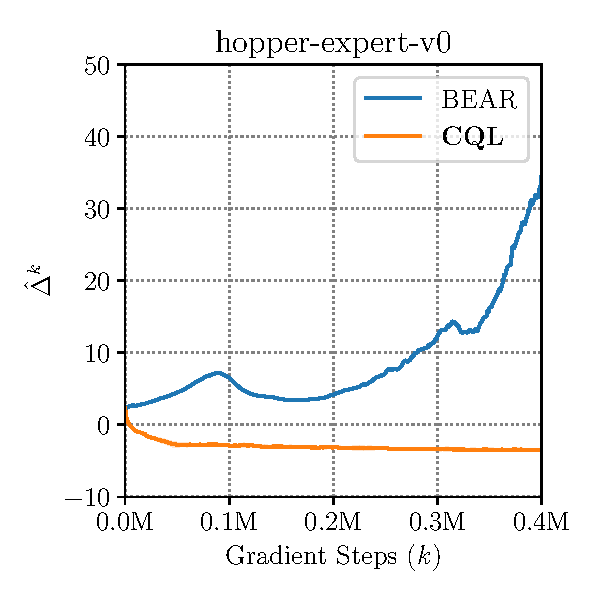
\includegraphics[width=0.47\linewidth]{NeuRIPS2019/images/hopper-expert-v0bear_vs_cql.pdf}
      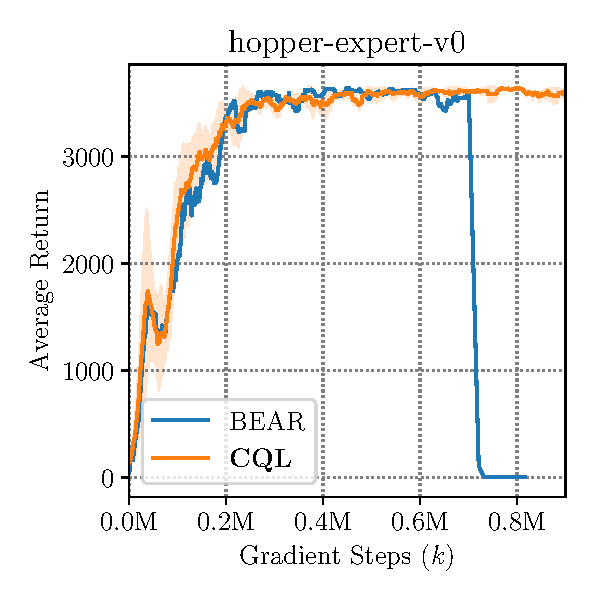
\includegraphics[width=0.47\linewidth]{NeuRIPS2019/images/hopper-expert-v0bear_vs_cql_return.pdf}
      \caption{hopper-expert-v0}
    \end{subfigure}
    ~
    \begin{subfigure}[h]{0.49\linewidth}
      \centering
      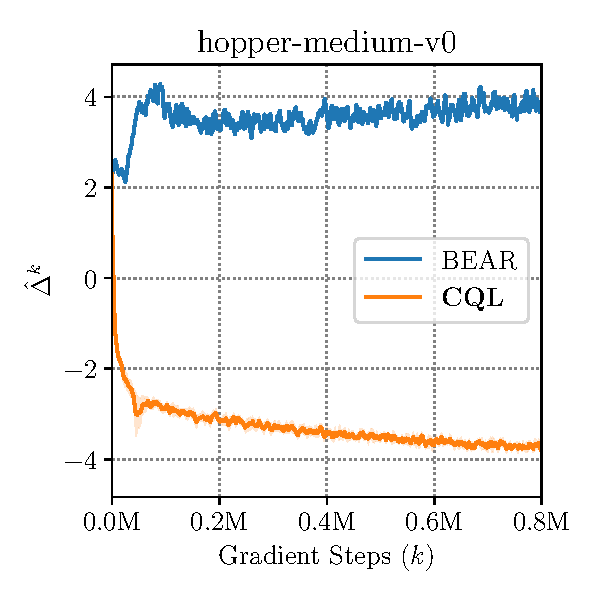
\includegraphics[width=0.47\linewidth]{NeuRIPS2019/images/hopper-medium-v0bear_vs_cql_again.pdf}
      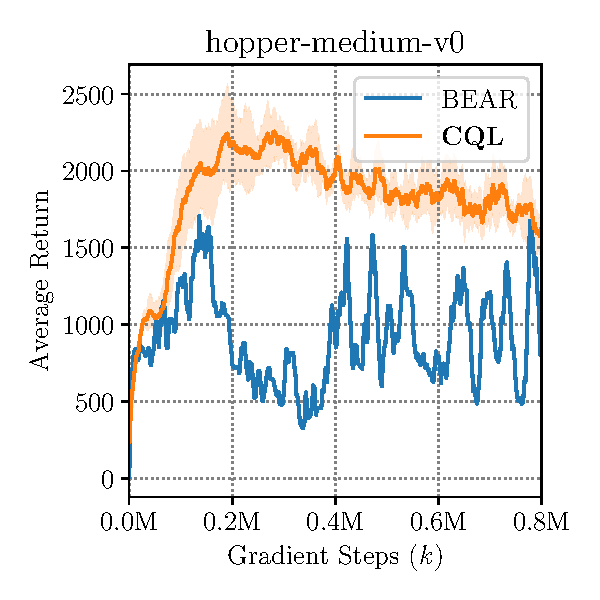
\includegraphics[width=0.47\linewidth]{NeuRIPS2019/images/hopper-medium-v0bear_vs_cql_again_return.pdf}
      \caption{hopper-medium-v0}
      %%SL.5.27: label the plots -- label both axes and title
    \end{subfigure}
    \caption{$\Delta^k$ as a function of training iterations for hopper-expert and hopper-medium datasets. Note that CQL (left) generally has negative values of $\Delta$, whereas BEAR (right) generally has positive $\Delta$ values, which also increase during training with increasing $k$ values.}
    %%SL.5.27: Make sure caption at least briefly summarizes the implications of this
    \label{fig:delta_plots}
\end{figure}

% \textbf{Why does CQL solve this problem?} Theorem~\ref{thm:gap_amplify} indicates that, by appropriately controlling for $\alpha_k$, CQL can ensure that the learned $\hat{\Delta}^k$ is larger than the actual value of $\Delta^k$ in the MDP (when evaluated using the true Q-function, $Q^k$). That is, for all $k$, we have that $\hat{\Delta}^k > \Delta^k$ under appropriate choices of $\alpha_1, \cdots, \alpha_k$. Empirically, this translates to generally negative (or positive with a small magnitude) values of $\hat{\Delta}^k$ for CQL, as shown in Figure~\ref{fig:delta_plots}(a) and (b). Note that it is sufficient for the empirical $\hat{\Delta}^k$ to be larger than $\Delta^k$, and not necessarily negative. 
% %%AK.5.26: Revisit this statement once.
% CQL generally maintains a negative value of $\hat{\Delta}^k$, and this difference is reflected in better and more stable final policy performance for CQL, as shown in Figure ??, even without a policy constraint. 


\vspace{-0.3cm}
\section{Theorem Proofs}
\label{app:missing_proofs}
\vspace{-0.3cm}

In this section, we provide proofs of the theorems in Sections~\ref{sec:policy_eval} and \ref{sec:framework}. We first redefine notation for clarity and then provide the proofs of the results in the main paper.

\textbf{Notation.} Let $k \in \mathbb{N}$ denote an iteration of policy evaluation (in Section~\ref{sec:policy_eval}) or Q-iteration (in Section~\ref{sec:framework}). In an iteration $k$, the objective -- Equation~\ref{eqn:modified_policy_eval} or Equation~\ref{eqn:cql_framework} -- is optimized using the previous iterate (i.e. $\hat{Q}^{k-1}$) as the target value in the backup. $Q^k$ denotes the true, tabular Q-function iterate in the MDP, without any correction. In an iteration, say $k+1$, the current tabular Q-function iterate, $Q^{k+1}$ is related to the previous tabular Q-function iterate ${Q}^k$ as: $Q^{k+1} = \bellman^{\policy} Q^k$ (for policy evaluation) or $Q^{k+1} = \bellman^{\policy_k} Q^k$ (for policy learning). Let $\hat{Q}^k$ denote the $k$-th Q-function iterate obtained from CQL. Let $\hat{V}^k$ denote the value function, $\hat{V}^k := \E_{\mathbf{a} \sim \policy(\mathbf{a}|\bs)}[\hat{Q}^k(\bs, \mathbf{a})]$.   

\textbf{A note on the value of $\alpha$.} Before proving the theorems, we remark that while the statements of Theorems~\ref{thm:cql_underestimates}, \ref{thm:min_q_underestimates} and \ref{thm:policy_eval_func_approx} (we discuss this in Appendix~\ref{app:additional_theory}) show that CQL produces lower bounds if $\alpha$ is larger than some threshold, so as to overcome either sampling error (Theorems~\ref{thm:cql_underestimates} and \ref{thm:min_q_underestimates}) or function approximation error (Theorem~\ref{thm:policy_eval_func_approx}). While the optimal $\alpha_k$ in some of these cases depends on the current Q-value, $\hat{Q}^k$, we can always choose a worst-case value of $\alpha_k$ by using the inequality $\hat{Q}^k \leq 2 R_{\max}/(1 - \gamma)$, still guaranteeing a lower bound. If it is unclear why the learned Q-function $\hat{Q}^k$ should be bounded, we can always clamp the Q-values if they go outside $\left[ \frac{-2 R_{\max}}{1 - \gamma}, \frac{2 R_{\max}}{1 - \gamma} \right]$.
We first prove Theorem~\ref{thm:min_q_underestimates}, which shows that policy evaluation using a simplified version of CQL (Equation~\ref{eqn:objective_1}) results in a point-wise lower-bound on the Q-function. 

~

\niparagraph{\large{Proof of Theorem~\ref{thm:min_q_underestimates}}} 


We start by analyzing $\hat{Q}^k$ by setting the derivative of Equation~\ref{eqn:objective_1} to 0:
\begin{equation}
    \forall~\bs, \mathbf{a} \in \mathcal{D}, k, ~~ \hat{Q}^{k+1}(\bs, \mathbf{a}) = \hat{\bellman}^\pi \hat{Q}^k(\bs, \mathbf{a}) - \alpha \frac{\mu(\mathbf{a}|\bs)}{\hatbehavior(\mathbf{a}|\bs)}.
    \label{eqn:q_expression_objective1}
\end{equation}
Now, since, $\mu(\mathbf{a}|\bs) > 0, \alpha > 0, \hatbehavior(\mathbf{a}|\bs) > 0$, we observe that at each iteration we underestimate the next Q-value iterate, i.e. $\hat{Q}^{k+1} \leq \hat{\bellman}^\policy \hat{Q}^k$.

\textbf{Accounting for sampling error.} Note that so far we have only shown that the Q-values are upper-bounded by the the ``empirical Bellman targets'' given by, $\hat{\bellman}^\policy \hat{Q}^k$. In order to relate $\hat{Q}^k$ to the true Q-value iterate, $Q^k$, we need to relate the empirical Bellman operator, $\hat{\bellman}^\policy$ to the actual Bellman operator, $\bellman^\policy$. In Appendix~\ref{app:handling_unobserved_actions}, we show that if the reward function $r(\bs, \mathbf{a})$ and the transition function, $\transitions(\bs'|\bs, \mathbf{a})$ satisfy ``concentration'' properties, meaning that the difference between the observed reward sample, $r$ ($\bs, \mathbf{a}, r, \bs') \in \mathcal{D}$) and the actual reward function $r(\bs, \mathbf{a})$ (and analogously for the transition matrix) is bounded with high probability, then overestimation due to the empirical Backup operator is bounded. Formally, with high probability (w.h.p.) $\geq 1 - \delta$, $\delta \in (0, 1)$, 
\begin{equation*}
    \forall Q, \bs, \mathbf{a} \in \mathcal{D},~~ \left\vert \hat{\bellman}^\policy Q(\bs, \mathbf{a}) - \bellman^\policy Q(\bs, \mathbf{a}) \right\vert \leq \frac{C_{r, T, \delta} R_{\max}}{(1 - \gamma) \sqrt{|\mathcal{D}(\bs, \mathbf{a})|}}.
\end{equation*}
Hence, the following can be obtained, w.h.p.:
\begin{align}
\label{eqn:pac_bound_q_value}
    \hat{Q}^{k+1}(\bs, \mathbf{a}) = \bellman^\policy \hat{Q}^k(\bs, \mathbf{a}) \leq \bellman^\policy \hat{Q}^k(\bs, \mathbf{a}) - \alpha \frac{\mu(\mathbf{a}|\bs)}{\hatbehavior(\mathbf{a}|\bs)} + \frac{C_{r, T, \delta} R_{\max}}{(1 - \gamma) \sqrt{|\mathcal{D}(\bs, \mathbf{a})|}}.
\end{align}

Now we need to reason about the fixed point of the update procedure in Equation~\ref{eqn:q_expression_objective1}. The fixed point of Equation~\ref{eqn:q_expression_objective1} is given by:
\begin{multline*}
    \hat{Q}^\policy \leq \bellman^\policy \hat{Q}^\policy - \alpha \frac{\mu(\mathbf{a}|\bs)}{\hatbehavior(\mathbf{a}|\bs)} + \frac{C_{r, T, \delta} R_{\max}}{(1 - \gamma) \sqrt{|\mathcal{D}(\bs, \mathbf{a})|}} \implies \hat{Q}^\pi \leq (I - \gamma P^\pi)^{-1} \left[ R  - \alpha \frac{\mu}{\hatbehavior} + \frac{C_{r, T, \delta} R_{\max}}{1 - \gamma) \sqrt{|\mathcal{D}}}\right]\\
    \hat{Q}^\policy(\bs, \mathbf{a}) \leq Q^\policy(\bs, \mathbf{a}) - \alpha \left[ \left(I - \gamma P^\pi \right)^{-1} \left[\frac{\mu}{\hatbehavior} \right] \right](\bs, \mathbf{a}) + \left[(I - \gamma P^\policy)^{-1} \frac{C_{r, T, \delta} R_{\max}}{(1 - \gamma) \sqrt{|\mathcal{D}|}} \right](\bs, \mathbf{a}),
\end{multline*}
thus proving the relationship in Theorem~\ref{thm:min_q_underestimates}.

In order to guarantee a lower bound, $\alpha$ can be chosen to cancel any potential overestimation incurred by $\frac{C_{r, T, \delta} R_{\max}}{(1 - \gamma)\sqrt{|\mathcal{D}|}}$. Note that this  choice works, since $(I - \gamma P^\pi)^{-1}$ is a matrix with all non-negative entries. The choice of $\alpha$ that guarantees a lower bound is then given by:
\begin{align*}
    \alpha& ~ \cdot \min_{\bs, \mathbf{a}} \left[\frac{\mu(\mathbf{a}|\bs)}{\hatbehavior(\mathbf{a}|\bs)} \right] \geq \max_{\bs, \mathbf{a}} \frac{C_{r, T, \delta} R_{\max}}{(1 - \gamma) \sqrt{|\mathcal{D}(\bs, \mathbf{a})|}}\\
    \implies \alpha&~ \geq \max_{\bs, \mathbf{a}} \frac{C_{r, T, \delta} R_{\max}}{(1 - \gamma) \sqrt{|\mathcal{D}(\bs, \mathbf{a})|}} \cdot \max_{\bs, \mathbf{a}} \left[\frac{\mu(\mathbf{a}|\bs)}{\hatbehavior(\mathbf{a}|\bs)} \right]^{-1}.
\end{align*}
Note that the theoretically minimum possible value of $\alpha$ decreases as more samples are observed, i.e., when $|\mathcal{D}(\bs, \mathbf{a})|$ is large. Also, note that since, $\frac{C_{r, T, \delta} R_{\max}}{(1 - \gamma0 \sqrt{|\mathcal{D}|}} \approx 0$, when $\hat{\bellman}^\policy = \bellman^\policy$, any $\alpha \geq 0$ guarantees a lower bound. And so choosing a value of $\alpha = 0$ is sufficient in this case.

Next, we prove Theorem~\ref{thm:cql_underestimation} that shows that the additional term that maximizes the expected Q-value under the dataset distribution, $\mathbb{D}(\bs, \mathbf{a})$, (or $d^\behavior(\bs) \behavior(\mathbf{a}|\bs)$, in the absence of sampling error), results in a lower-bound on only the expected value of the policy at a state, and not a pointwise lower-bound on Q-values at all actions.

~

\niparagraph{\large{Proof of Theorem~\ref{thm:cql_underestimates}}} 


We first prove this theorem in the absence of sampling error, and then incorporate sampling error at the end, using a technique similar to the previous proof. In the tabular setting, we can set the derivative of the modified objective in Equation~\ref{eqn:modified_policy_eval}, and compute the Q-function update induced in the exact, tabular setting (this assumes $\hat{\bellman}^\policy = \bellman^\policy)$ and $\behavior(\mathbf{a}|\bs) = \hatbehavior(\mathbf{a}|\bs)$).
\begin{equation}
    \forall ~\bs, \mathbf{a}, k ~~ \hat{Q}^{k+1} (\bs, \mathbf{a}) = \bellman^\policy \hat{Q}^k(\bs, \mathbf{a}) - \alpha \left[\frac{\mu(\mathbf{a}|\bs)}{\behavior(\mathbf{a}|\bs)} - 1 \right].
    \label{eqn:q_function_modified_eval}
\end{equation}
Note that for state-action pairs, $(\bs, \mathbf{a})$, such that, $\mu(\mathbf{a}|\bs) < \behavior(\mathbf{a}|\bs)$, we are infact adding a positive quantity, $1 - \frac{\mu(\mathbf{a}|\bs)}{\behavior(\mathbf{a}|\bs)}$, to the Q-function obtained, and this we cannot guarantee a point-wise lower bound, i.e. $\exists~ \bs, \mathbf{a}, \text{~~s.t.}~~ \hat{Q}^{k+1}(\bs, \mathbf{a}) \geq Q^{k+1}(\bs, \mathbf{a})$. To formally prove this, we can construct a counter-example three-state, two-action MDP, and choose a specific behavior policy $\policy(\mathbf{a}|\bs)$, such that this is indeed the case.

The value of the policy, on the other hand, $\hat{V}^{k+1}$ is underestimated, since:
\begin{equation}
    \hat{V}^{k+1}(\bs) := \E_{\mathbf{a} \sim \policy(\mathbf{a}|\bs)} \left[ \hat{Q}^{k+1}(\bs, \mathbf{a}) \right] = \bellman^\policy \hat{V}^k (\bs) - \alpha \E_{\mathbf{a} \sim \policy(\mathbf{a}|\bs)}\left[\frac{\mu(\mathbf{a}|\bs)}{\behavior(\mathbf{a}|\bs)} - 1 \right].
    \label{eqn:value_recursion}
\end{equation}
and we can show that $D_{\text{CQL}}(\bs): = \sum_{\mathbf{a}} \policy(\mathbf{a}|\bs) \left[\frac{\mu(\mathbf{a}|\bs)}{\behavior(\mathbf{a}|\bs)} - 1 \right]$ is always positive, when $\policy(\mathbf{a}|\bs) = \mu(\mathbf{a}|\bs)$. To note this, we present the following derivation:
\begin{align*}
    D_{\text{CQL}}(\bs) &:=~ \sum_{\mathbf{a}} \policy(\mathbf{a}|\bs) \left[\frac{\mu(\mathbf{a}|\bs)}{\behavior(\mathbf{a}|\bs)} - 1 \right]\\
    &= \sum_{\mathbf{a}} (\policy(\mathbf{a}|\bs) - \behavior(\mathbf{a}|\bs) + \behavior(\mathbf{a}|\bs)) \left[\frac{\mu(\mathbf{a}|\bs)}{\behavior(\mathbf{a}|\bs)} - 1 \right]\\
    &= \sum_{\mathbf{a}} (\policy(\mathbf{a}|\bs) - \behavior(\mathbf{a}|\bs)) \left[ \frac{\policy(\mathbf{a}|\bs) - \behavior(\mathbf{a}|\bs)}{\behavior(\mathbf{a}|\bs} \right] + \sum_{\mathbf{a}} \behavior(\mathbf{a}|\bs) \left[\frac{\mu(\mathbf{a}|\bs)}{\behavior(\mathbf{a}|\bs)} - 1 \right]\\
    &= \sum_{\mathbf{a}} \underbrace{\left[ \frac{\left(\policy(\mathbf{a}|\bs) - \behavior(\mathbf{a}|\bs) \right)^2}{\behavior(\mathbf{a}|\bs)} \right]}_{\geq 0}~ +~ 0 \text{~~~since,~} \sum_{\mathbf{a}} \policy(\mathbf{a}|\bs) = \sum_{\mathbf{a}} \behavior(\mathbf{a}|\bs) = 1.
\end{align*}
Note that the marked term, is positive since both the numerator and denominator are positive, and this implies that $D_\text{CQL}(\bs) \geq 0$. Also, note that $D_\text{CQL}(\bs) = 0$, iff $\policy(\mathbf{a}|\bs) = \behavior(\mathbf{a}|\bs)$. This implies that each value iterate incurs some underestimation, $\hat{V}^{k+1}(\bs) \leq \bellman^\policy \hat{V}^k (\bs)$.

Now, we can compute the fixed point of the recursion in Equation~\ref{eqn:value_recursion}, and this gives us the following estimated policy value:
\begin{equation*}
    \hat{V}^\policy(\bs) = V^\policy(\bs) - \alpha \left[ \underbrace{(I - \gamma P^\policy)^{-1}}_{\text{non-negative entries}}
    \underbrace{\E_{\policy}\left[\frac{\policy}{\behavior} - 1 \right]}_{\geq 0} \right](\bs),
\end{equation*}
thus showing that in the absence of sampling error, Theorem~\ref{thm:cql_underestimates} gives a lower bound. It is straightforward to note that this expression is tighter than the expression for policy value in Proposition~\ref{thm:cql_underestimates}, since, we explicitly subtract $1$ in the expression of Q-values from the previous proof.

\textbf{Incorporating sampling error.} To extend this result to the setting with sampling error, similar to the previous result, the maximal overestimation at each iteration $k$, is bounded by $\frac{C_{r, T, \delta} R_{\max}}{1 - \gamma}$.
The resulting value-function satisfies (w.h.p.), $\forall \bs \in \mathcal{D}$, 
\begin{equation*}
   \hat{V}^\policy(\bs) \leq V^\policy(\bs) - \alpha \left[\left(I - \gamma P^\pi \right)^{-1} \E_{\policy}\left[\frac{\policy}{\hatbehavior} - 1 \right] \right](\bs) + \left[ (I - \gamma P^\pi)^{-1} \frac{C_{r, T, \delta} R_{\max}}{(1- \gamma) \sqrt{|\mathcal{D}|}}\right](\bs)
\end{equation*}
thus proving the theorem statement. In this case, the choice of $\alpha$, that prevents overestimation w.h.p. is given by:
\begin{equation*}
    \alpha \geq \max_{\bs, \mathbf{a} \in \mathcal{D}} \frac{C_{r, T} R_{\max}}{(1 - \gamma) \sqrt{|\mathcal{D}(\bs, \mathbf{a})|}} \cdot \max_{\bs \in \mathcal{D}} \left[\sum_{\mathbf{a}} \policy(\mathbf{a}|\bs) \left(\frac{\policy(\mathbf{a}|\bs)}{\hatbehavior(\mathbf{a}|\bs))} - 1\right)\right]^{-1}.
\end{equation*}
Similar to Theorem~\ref{thm:min_q_underestimates}, note that the theoretically acceptable value of $\alpha$ decays as the number of occurrences of a state action pair in the dataset increases.
Next we provide a proof for Theorem~\ref{thm:cql_underestimation}.

~

\niparagraph{\large{Proof of Theorem~\ref{thm:cql_underestimation}}} 

In order to prove this theorem, we compute the difference induced in the policy value, $\hat{V}^{k+1}$, derived from the Q-value iterate, $\hat{Q}^{k+1}$, with respect to the previous iterate $\bellman^\policy \hat{Q}^{k}$. If this difference is negative at each iteration, then the resulting Q-values are guaranteed to lower bound the true policy value.

\begin{align*}
    \E_{\hat{\policy}^{k+1}(\mathbf{a}|\bs)}[\hat{Q}^{k+1}(\bs, \mathbf{a})] &=  \E_{\hat{\policy}^{k+1}(\mathbf{a}|\bs)}\left[ \bellman^\policy \hat{Q}^k (\bs, \mathbf{a}) \right] - \E_{\hat{\policy}^{k+1}(\mathbf{a}|\bs)}\left[ \frac{\pi_{\hat{Q}^k}(\mathbf{a} | \bs)}{\hatbehavior(\mathbf{a}|\bs)} -1 \right]\\
    &= \E_{\hat{\policy}^{k+1}(\mathbf{a}|\bs)}\left[ \bellman^\policy \hat{Q}^k (\bs, \mathbf{a}) \right] - \underbrace{\E_{\policy_{\hat{Q}^k}(\mathbf{a} | \bs)}\left[ \frac{\policy_{\hat{Q}^k}(\mathbf{a} | \bs)}{\hatbehavior(\mathbf{a}|\bs)} -1 \right]}_{\text{underestimation, ~~(a)}}\\
    &~~~~~~~~~~~~~~~~~~~~~~~~~~~~~+ \sum_{\mathbf{a}} \underbrace{\left(\policy_{\hat{Q}^k}(\mathbf{a} | \bs) - \hat{\policy}^{k+1}(\mathbf{a}|\bs) \right)}_{\text{(b),}~~{\leq \mathrm{D_{TV}}(\policy_{\hat{Q}^k}, \hat{\policy}^{k+1})}} \frac{\policy_{\hat{Q}^k}(\mathbf{a} | \bs)}{\hatbehavior(\mathbf{a}|\bs)}
    %   \E_{\pi_{\hat{Q}^k}(\mathbf{a} | \bs)}[\hat{Q}^{k+1}(\bs, \mathbf{a})] - 
\end{align*}
If (a) has a larger magnitude than (b), then the learned Q-value induces an underestimation in an iteration $k+1$, and hence, by a recursive argument, the learned Q-value underestimates the optimal Q-value. We note that by upper bounding term (b) by $\mathrm{D_{TV}}(\policy_{\hat{Q}^k}, \hat{\policy}^{k+1}) \cdot \max_{\mathbf{a}} \frac{\policy_{\hat{Q}^k}(\mathbf{a} | \bs)}{\hatbehavior(\mathbf{a}|\bs)}$, and writing out (a) > upper-bound on (b), we obtain the desired result.


Finally, we show that under specific choices of $\alpha_1, \cdots, \alpha_k$, the CQL backup is gap-expanding by providing a proof for Theorem~\ref{thm:gap_amplify}.

~

\niparagraph{\large{Proof of Theorem~\ref{thm:gap_amplify} (CQL is gap-expanding)}}

For this theorem, we again first present the proof in the absence of sampling error, and then incorporate sampling error into the choice of $\alpha$. We follow the strategy of observing the Q-value update in one iteration. Recall that the expression for the Q-value iterate at iteration $k$ is given by:
\begin{equation*}
    \hat{Q}^{k+1}(\bs, \mathbf{a}) = \bellman^{\policy^k} \hat{Q}^{k}(\bs, \mathbf{a}) - \alpha_k \frac{\mu_k(\mathbf{a}|\bs) - \behavior(\mathbf{a}|\bs)}{\behavior(\mathbf{a}|\bs)}.
\end{equation*}
Now, the value of the policy $\mu_{k}(\mathbf{a}|\bs)$ under $\hat{Q}^{k+1}$ is given by:
\begin{equation*}
    \E_{\mathbf{a} \sim \mu_k(\mathbf{a}|\bs)}[\hat{Q}^{k+1}(\bs, \mathbf{a})] = \E_{\mathbf{a} \sim \mu_k(\mathbf{a}|\bs)}[\bellman^{\policy^k} \hat{Q}^k (\bs, \mathbf{a})] - \alpha_k \underbrace{\mu_k^T \left(\frac{\mu_k(\mathbf{a}|\bs) - \behavior(\mathbf{a}|\bs)}{\behavior(\mathbf{a}|\bs)} \right)}_{:= \hat{\Delta}^k, \geq 0, \text{~~by proof of Theorem~\ref{thm:cql_underestimates}.}} 
\end{equation*}
Now, we also note that the expected amount of extra underestimation introduced at iteration $k$ under action sampled from the behavior policy $\behavior(\mathbf{a}|\bs)$ is 0, as,
\begin{equation*}
    \E_{\mathbf{a} \sim \behavior(\mathbf{a}|\bs)}[\hat{Q}^{k+1}(\bs, \mathbf{a})] = \E_{\mathbf{a} \sim \behavior(\mathbf{a}|\bs)}[\bellman^{\policy^k} \hat{Q}^k (\bs, \mathbf{a})] - \alpha_k \underbrace{\behavior^T \left(\frac{\mu_k(\mathbf{a}|\bs) - \behavior(\mathbf{a}|\bs)}{\behavior(\mathbf{a}|\bs)} \right)}_{= 0}. 
\end{equation*}
where the marked quantity is equal to 0 since it is equal since $\behavior(\mathbf{a}|\bs)$ in the numerator cancels with the denominator, and the remaining quantity is a sum of difference between two density functions, $\sum_{\mathbf{a}} \mu_k(\mathbf{a}|\bs) - \behavior(\mathbf{a}|\bs)$, which is equal to 0. Thus, we have shown that,
\begin{equation*}
    \E_{\behavior(\mathbf{a}|\bs)}[\hat{Q}^{k+1}(\bs, \mathbf{a})] - \E_{\mu_k(\mathbf{a}|\bs)}[\hat{Q}^{k+1}(\bs, \mathbf{a})] = \E_{\behavior(\mathbf{a}|\bs)}[\bellman^{\policy^k} \hat{Q}^k (\bs, \mathbf{a})] - \E_{\mu_k(\mathbf{a}|\bs)}[\bellman^{\policy^k} \hat{Q}^k (\bs, \mathbf{a})] - \alpha_k \hat{\Delta}^k.
\end{equation*}
Now subtracting the difference, $\E_{\behavior(\mathbf{a}|\bs)}[Q^{k+1}(\bs, \mathbf{a})] - \E_{\mu_k(\mathbf{a}|\bs)}[Q^{k+1}(\bs, \mathbf{a})]$, computed under the tabular Q-function iterate, $Q^{k+1}$, from the previous equation, we obtain that
\begin{multline*}
    \E_{\mathbf{a} \sim \behavior(\mathbf{a}|\bs)}[\hat{Q}^{k+1}(\bs, \mathbf{a})] - \E_{\behavior(\mathbf{a}|\bs)}[{Q}^{k+1}(\bs, \mathbf{a})] = \E_{\mu_k(\mathbf{a}|\bs)}[\hat{Q}^{k+1}(\bs, \mathbf{a})] - \E_{\mu_k(\mathbf{a}|\bs)}[{Q}^{k+1}(\bs, \mathbf{a})]\\
    + (\mu_k(\mathbf{a}|\bs) - \behavior(\mathbf{a}|\bs))^T \underbrace{\left[ \bellman^{\policy^k} \left( \hat{Q}^k - Q^k \right)(\bs, \cdot) \right]}_{(a)}- \alpha_k \hat{\Delta}^k.
\end{multline*}
% Now, by invoking Theorem~\ref{thm:cql_underestimation}, we note that the quantity marked as (a) in the previous equation is negative, since it is the expected difference between $\hat{Q}^k - \hat{Q}^k$ under the policy iterate, $\policy^k$. 

Now, by choosing $\alpha_k$, such that any positive bias introduced by the quantity $(\mu_k(\mathbf{a}|\bs) - \behavior(\mathbf{a}|\bs))^T (a)$ is cancelled out, we obtain the following gap-expanding relationship:
\begin{equation*}
    \E_{\mathbf{a} \sim \behavior(\mathbf{a}|\bs)}[\hat{Q}^{k+1}(\bs, \mathbf{a})] - \E_{\behavior(\mathbf{a}|\bs)}[{Q}^{k+1}(\bs, \mathbf{a})] > \E_{\mu_k(\mathbf{a}|\bs)}[\hat{Q}^{k+1}(\bs, \mathbf{a})] - \E_{\mu_k(\mathbf{a}|\bs)}[{Q}^{k+1}(\bs, \mathbf{a})]
\end{equation*}
for, $\alpha_k$ satisfying, 
\begin{equation*}
    \alpha_k > \max \left(\frac{(\behavior(\mathbf{a}|\bs) - \mu_k(\mathbf{a}|\bs))^T \left[ \bellman^{\policy^k} \left( \hat{Q}^k - Q^k \right)(\bs, \cdot) \right]}{\hat{\Delta}^k}, 0\right),
\end{equation*}
thus proving the desired result.

To avoid the dependency on the true Q-value iterate, ${Q}^k$, we can upper-bound $Q^k$ by $\frac{R_{\max}}{1 - \gamma}$, and upper-bound $(\behavior(\mathbf{a}|\bs) - \mu_k(\mathbf{a}|\bs))^T \bellman^{\policy^k} Q^k (\bs, \cdot)$ by $D_{\mathrm{TV}}(\behavior, \mu_k) \cdot \frac{R_{\max}}{1 - \gamma}$, and use this in the expression for $\alpha_k$. While this bound may be loose, it still guarantees the gap-expanding property, and we indeed empirically show the existence of this property in practice in Appendix~\ref{app:gap_amplify}. 

To incorporate sampling error, we can follow a similar strategy as previous proofs: the worst case overestimation due to sampling error is given by $\frac{C_{r, T, \delta} R_{\max}}{1 - \gamma}$. In this case, we note that, w.h.p.,
\begin{equation*}
    \left\vert \hat{\bellman}^{\policy^k} \left( \hat{Q}^k - Q^k \right) - \bellman^{\policy^k} \left( \hat{Q}^k - Q^k \right) \right\vert \leq \frac{2 \cdot C_{r, T, \delta} R_{\max}}{1 - \gamma}. 
\end{equation*}
Hence, the presence of sampling error adds $D_{\mathrm{TV}}(\hat{\behavior}, \mu_k) \cdot \frac{2 \cdot C_{r, T, \delta} R_{\max}}{1 - \gamma}$ to the value of $\alpha_k$, giving rise to the following, sufficient condition on $\alpha_k$ for the gap-expanding property:
\begin{equation*}
     \alpha_k > \max \left(\frac{(\behavior(\mathbf{a}|\bs) - \mu_k(\mathbf{a}|\bs))^T \left[ \bellman^{\policy^k} \left( \hat{Q}^k - Q^k \right)(\bs, \cdot) \right]}{\hat{\Delta}^k} + D_{\mathrm{TV}}(\hat{\behavior}, \mu_k) \cdot \frac{2 \cdot C_{r, T, \delta} R_{\max}}{1 - \gamma}, 0\right),
\end{equation*}
concluding the proof of this theorem.

% \vspace{-0.1cm}
\section{Additional Theoretical Analysis}
\label{app:additional_theory}
% \vspace{-0.2cm}

In this section, we present a theoretical analysis of additional properties of CQL. For ease of presentation, we state and prove theorems in Appendices~\ref{app:cql_linear_non_linear} and \ref{app:maximizing_distributions} in the absence of sampling error, but as discussed extensively in Appendix~\ref{app:missing_proofs}, we can extend each of these results by adding extra terms induced due to sampling error. 

\subsection{CQL with Linear and Non-Linear Function Approximation}
\label{app:cql_linear_non_linear}
\begin{theorem}
\label{thm:policy_eval_func_approx}
Assume that the Q-function is represented as a linear function of given state-action feature vectors $\Qfeat$, i.e., $Q(s, a) = w^T \Qfeat(s, a)$. Let $D = \text{diag}\left(d^\behavior(\bs) \behavior(\mathbf{a}|\bs)\right)$ denote the diagonal matrix with data density, and assume that $\Qfeat^T D \Qfeat$ is invertible. Then, the expected value of the policy under Q-value from Eqn~\ref{eqn:modified_policy_eval} at iteration $k+1$, $\E_{d^\behavior(\mathbf{a})}[\hat{V}^{k+1}(\bs)] = \E_{d^\behavior(\bs), \policy(\mathbf{a}|\bs)}[\hat{Q}^{k+1}(\bs, \mathbf{a})]$, lower-bounds the corresponding tabular value, $\E_{d^\behavior(\bs)}[V^{k+1}(\bs)] =\E_{d^\behavior(\bs), \policy(\mathbf{a}|\bs)}[Q^{k+1}(\bs, \mathbf{a})]$, if
\begin{equation*}
\small{\alpha_k \geq \max \left(\frac{D^T\left[\Qfeat \left(\Qfeat^T D \Qfeat \right)^{-1} \Qfeat^T - I \right]\left((\bellman^\policy \hat{Q}^k)(\bs, \mathbf{a})\right)}{D^T\left[ \Qfeat \left(\Qfeat^T D \Qfeat \right)^{-1} \Qfeat^T \right] \left(D \left[\frac{\policy(\mathbf{a}|\bs) - \behavior(\mathbf{a}|\bs)}{\behavior(\mathbf{a}|\bs)} \right] \right)},~ 0 \right).}
    %  \small{\alpha_k \geq \max \left(\frac{\left(d^\behavior(\bs) \mu(\mathbf{a}|\bs)\right)^T\left[\Qfeat \left(\Qfeat^T D \Qfeat \right)^{-1} \Qfeat^T - I \right]\left((\bellman^\policy \hat{Q}^k)(\bs, \mathbf{a})\right)}{\left(d^\behavior(\bs) \mu(\mathbf{a}|\bs)\right)^T\left[ \Qfeat \left(\Qfeat^T D \Qfeat \right)^{-1} \Qfeat^T \right] \left(d^\behavior(\bs) \left( \mu(\mathbf{a}|\bs) - \behavior(\mathbf{a}|\bs) \right) \right)},~ 0 \right).}
\end{equation*}
\end{theorem}
%intuitive justification for the theorem
The choice of $\alpha_k$ in Theorem~\ref{thm:policy_eval_func_approx} intuitively amounts to compensating for overestimation in value induced if the true value function cannot be represented in the chosen linear function class (numerator), by the potential decrease in value due to the CQL regularizer (denominator). This implies that if the actual value function can be represented in the linear function class, such that the numerator can be made $0$, then \textbf{any} $\alpha > 0$ is sufficient to obtain a lower bound. We now prove the theorem.

\begin{proof} 
In order to extend the result of Theorem~\ref{thm:cql_underestimates} to account for function approximation, we follow the similar recipe as before. We obtain the optimal solution to the optimization problem below in the family of linearly expressible Q-functions, i.e. $\mathcal{Q} := \{\Qfeat w | w \in \mathbb{R}^{dim(\Qfeat)} \}$. 
\begin{equation*}
    \min_{Q \in \mathcal{Q}}~~ \alpha_k \cdot \left(\E_{d^\behavior(\bs),\mu(\mathbf{a}|\bs)}\left[Q(\bs, \mathbf{a})\right] - {\E_{d^\behavior(\bs),\behavior(\mathbf{a}|\bs)}\left[Q(\bs, \mathbf{a})\right]} \right) + \frac{1}{2}~ \E_{\mathcal{D}}\left[\left(Q(\bs, \mathbf{a}) - \bellman^\policy \hat{Q}^{k} (\bs, \mathbf{a}) \right)^2 \right].
\end{equation*}
By substituting $Q(\bs, \mathbf{a}) = w^T \Qfeat(\bs, \mathbf{a})$, and setting the derivative with respect to $w$ to be 0, we obtain,
\begin{align*}
    \alpha \sum_{\bs, \mathbf{a}} d^\behavior(\bs) \cdot \left( \mu(\mathbf{a}|\bs) - \behavior(\mathbf{a}|\bs) \right) \Qfeat(\bs, \mathbf{a}) + \sum_{\bs, \mathbf{a}} d^\behavior(\bs) \behavior(\mathbf{a}|\bs) \left( Q(\bs, \mathbf{a}) - \bellman^\pi \hat{Q}^k(\bs, \mathbf{a}) \right) \Qfeat(\bs, \mathbf{a}) = 0.
\end{align*}
By re-arranging terms, and converting it to vector notation, defining $D = \text{diag}(d^\behavior(\bs)\behavior(\bs))$, and referring to the parameter $w$ at the k-iteration as $w^k$ we obtain:
\begin{align*}
    \left(\Qfeat^T D \Qfeat \right) w^{k+1} = \underbrace{\Qfeat^T D \left( \bellman^\policy \hat{Q}^k \right)}_{\text{LSTD iterate}} - \underbrace{\alpha_k \Qfeat^T \text{diag}\left[d^\behavior(\bs) \cdot(\mu(\mathbf{a}|\bs) - \behavior(\mathbf{a}|\bs)) \right]}_{\text{underestimation}}.
\end{align*}
Now, our task is to show that the term labelled as ``underestimation'' is indeed negative in expectation under $\mu(\mathbf{a}|\bs)$ (This is analogous to our result in the tabular setting that shows underestimated values). In order to show this, we write out the expression for the value, under the linear weights $w^{k+1}$ at state $\bs$, after substituting $\mu = \policy$,
\begin{align}
    \hat{V}^{k+1}(\bs) &:= \policy(\mathbf{a}|\bs)^T \Qfeat w^{k+1}\\
    = \policy(&\mathbf{a}|\bs)^T \underbrace{\Qfeat \left(\Qfeat^T D \Qfeat \right)^{-1} \Qfeat^T D \left(\bellman^\policy \hat{Q}^k \right)}_{\text{value under LSTD-Q~\citep{lagoudakis2003least}}} - \alpha_k \policy(\mathbf{a}|\bs)^T \Qfeat \left(\Qfeat^T D \Qfeat \right)^{-1} \Qfeat^T D \left[\frac{\policy(\mathbf{a}|\bs) - \behavior(\mathbf{a}|\bs)}{\behavior(\mathbf{a}|\bs)} \right].
    \label{expr:lstdq_value}
\end{align}
Now, we need to reason about this additional penalty term. Defining, $P_\Qfeat := \Qfeat \left(\Qfeat^T D \Qfeat \right)^{-1} \Qfeat^T D$ as the projection matrix onto the subspace of features $\Qfeat$, we need to show that the product that appears as a penalty is positive: $\policy(\mathbf{a}|\bs)^T P_\Qfeat \left[\frac{\policy(\mathbf{a}|\bs) - \behavior(\mathbf{a}|\bs)}{\behavior(\mathbf{a}|\bs)} \right] \geq 0$. In order to show this, we compute minimum value of this product optimizing over $\policy$. If the minimum value is $0$, then we are done.

Let's define $f(\policy) = \policy(\mathbf{a}|\bs)^T P_\Qfeat \left[\frac{\policy(\mathbf{a}|\bs) - \behavior(\mathbf{a}|\bs)}{\behavior(\mathbf{a}|\bs)} \right]$, our goal is to solve for $\min_{\policy} f(\policy)$. Setting the derivative of $f(\policy)$ with respect to $\policy$ to be equal to 0, we obtain (including Lagrange multiplier $\eta$ that guarantees $\sum_{\mathbf{a}} \policy(\mathbf{a}|\bs) = 1$,
\begin{equation*}
    \left( P_\Qfeat + P_\Qfeat^T \right) \left[\frac{\policy(\mathbf{a}|\bs)}{\behavior(\mathbf{a}|\bs)}\right] = P_\Qfeat \Vec{1} + \eta \Vec{1}.
\end{equation*}
By solving for $\eta$ (using the condition that a density function sums to 1), we obtain that the minimum value of $f(\policy)$ occurs at a $\policy^*(\mathbf{a}|\bs)$, which satisfies the following condition,
\begin{equation*}
    \left(P_\Qfeat + P_\Qfeat^T \right) \left[\frac{\policy^*(\mathbf{a}|\bs)}{\behavior(\mathbf{a}|\bs)}\right] = \left( P_\Qfeat + P_\Qfeat^T \right) \Vec{1}.
\end{equation*}
Using this relation to compute $f$, we obtain, $f(\policy^*) = 0$, indicating that the minimum value of $0$ occurs when the projected density ratio matches under the matrix $(P_\Qfeat + P_\Qfeat^T)$ is equal to the projection of a vector of ones, $\Vec{1}$. Thus, \begin{equation*}
    \forall~ \policy(\mathbf{a}|\bs),~ f(\policy) = \policy(\mathbf{a}|\bs)^T P_{\Qfeat} \left[\frac{\policy(\mathbf{a}|\bs) - \behavior(\mathbf{a}|\bs)}{\behavior(\mathbf{a}|\bs)} \right] \geq 0.
\end{equation*}

This means that: $\forall ~\bs, \hat{V}^{k+1}(\bs) \leq \hat{V}^{k+1}_{\text{LSTD-Q}}(\bs)$ given identical previous $\hat{Q}^{k}$ values. This result indicates, that if $\alpha_k \geq 0$, the resulting CQL value estimate with linear function approximation is guaranteed to lower-bound the value estimate obtained from a least-squares temporal difference Q-learning algorithm (which only minimizes Bellman error assuming a linear Q-function parameterization), such as LSTD-Q~\citep{lagoudakis2003least}, since at each iteration, CQL induces a lower-bound with respect to the previous value iterate, whereas this underestimation is absent in LSTD-Q. Also note that we can also apply an inductive argument.

So far, we have only shown that the learned value iterate, $\hat{V}^{k+1}(\bs)$ lower-bounds the value iterate obtained from LSTD-Q, $\forall ~\bs, \hat{V}^{k+1}(\bs) \leq \hat{V}^{k+1}_{\text{LSTD-Q}}(\bs)$. But, our final aim is to prove a stronger result, that the learned value iterate, $\hat{V}^{k+1}$, lower bounds the exact tabular value function iterate, ${V}^{k+1}$, at each iteration. The reason why our current result does not guarantee this is because function approximation may induce overestimation error in the linear approximation of the Q-function.

In order to account for this change, we make a simple change: we choose $\alpha_k$ such that the resulting penalty nullifes the effect of any over-estimation caused due to the inability to fit the true value function iterate in the linear function class parameterized by $\Qfeat$. Formally, this means:
\begin{align*}
    \E_{d^\behavior(\bs)}\left[\hat{V}^{k+1}(\bs)\right] &\leq \E_{d^\behavior(\bs)}\left[\hat{V}^{k+1}_{\text{LSTD-Q}}(\bs)\right] - \alpha_k \E_{d^\behavior(\bs)}[f(\policy(\mathbf{a}|\bs))] \\
    & \leq \E_{d^\behavior(\bs)}\left[V^{k+1}(\bs)\right] - \underbrace{\E_{d^\behavior(\bs)}\left[\hat{V}^{k+1}_{\text{LSTD-Q}}(\bs) - V^{k+1}(\bs) \right] - \alpha_k \E_{d^\behavior(\bs)}[f(\policy(\mathbf{a}|\bs))]}_{\text{choose~} \alpha_k \text{~to make this negative}} \\
    & \leq \E_{d^\behavior(\bs)}\left[V^{k+1}(\bs)\right]
\end{align*}
And the choice of $\alpha_k$ in that case is given by:
\begin{align*}
    \alpha_k \geq& ~ \max \left(\frac{\E_{d^\behavior(\bs)}\left[\hat{V}^{k+1}_{\text{LSTD-Q}}(\bs) - V^{k+1}(\bs) \right]}{\E_{d^\behavior(\bs)}[f(\policy(\mathbf{a}|\bs))]}, 0 \right)\\
    \geq& ~ \max \left(\frac{D^T\left[\Qfeat \left(\Qfeat^T D \Qfeat \right)^{-1} \Qfeat^T - I \right]\left((\bellman^\policy \hat{Q}^k)(\bs, \mathbf{a})\right)}{D^T\left[ \Qfeat \left(\Qfeat^T D \Qfeat \right)^{-1} \Qfeat^T \right] \left(D \left[\frac{\policy(\mathbf{a}|\bs) - \behavior(\mathbf{a}|\bs)}{\behavior(\mathbf{a}|\bs)} \right] \right)},~ 0 \right).
\end{align*}
Finally, we note that since this choice of $\alpha_k$ induces under-estimation in the next iterate, $\hat{V}^{k+1}$ with respect to the previous iterate, $\hat{V}^k$, for all $k \in \mathbb{N}$, by induction, we can claim that this choice of $\alpha_1, \cdots, \alpha_k$ is sufficient to make $\hat{V}^{k+1}$ lower-bound the tabular, exact value-function iterate. $V^{k+1}$, for all $k$, thus completing our proof.
\end{proof}
% done

We can generalize Theorem~\ref{thm:policy_eval_func_approx} to non-linear function approximation, such as neural networks, {under the standard NTK framework~\citep{ntk}}, assuming that each iteration $k$ is performed by a single step of gradient descent on Equation~\ref{eqn:modified_policy_eval}, rather than a complete minimization of this objective. As we show in Theorem~\ref{corr:nonlinear_ntk}, CQL learns lower bounds in this case for an appropriate choice of $\alpha_k$. 
% We will also empirically show in Appendix~\ref{app:cql_additional_results} that CQL can learn effective conservative Q-functions with multilayer neural networks.

%%SL.5.30: I don't think this should be called a corollary. Corollaries are supposed to quick and easy to prove, if it takes the better part of a page to prove, it's not a corollary.
\begin{theorem}[Extension to non-linear function approximation]
\label{corr:nonlinear_ntk}
Assume that the Q-function is represented by a general non-linear function approximator parameterized by $\theta$, $Q_\theta(\bs, \mathbf{a})$. let $D = \text{diag}(d^\behavior(\bs) \behavior(\mathbf{a}|\bs))$ denote the matrix with the data density on the diagonal, and assume that $\nabla_\theta Q_\theta^T D \nabla_\theta Q_\theta$ is invertible. Then, the expected value of the policy under the Q-function obtained by taking a gradient step on Equation~\ref{eqn:modified_policy_eval}, at iteration $k+1$ lower-bounds the corresponding tabular function iterate if: 
\end{theorem}

\begin{proof} Our proof strategy is to reduce the non-linear optimization problem into a linear one, with features $\Qfeat$ (in Theorem~\ref{thm:policy_eval_func_approx}) replaced with features given by the gradient of the current Q-function $\hat{Q}^{k}_\theta$ with respect to parameters $\theta$, i.e. $\nabla_\theta \hat{Q}^k$. To see, this we start by writing down the expression for $\hat{Q}^{k+1}_\theta$ obtained via one step of gradient descent with step size $\eta$, on the objective in Equation~\ref{eqn:modified_policy_eval}.
\begin{align*}
    \theta^{k+1} = \theta^k &- \eta \alpha_k \left( \E_{d^\behavior(\bs), \mu(\mathbf{a}|\bs)}\left[\nabla_\theta \hat{Q}^{k}(\bs, \mathbf{a})\right] - \E_{d^\behavior(\bs), \behavior(\mathbf{a}|\bs)}\left[\nabla_\theta \hat{Q}^{k}(\bs, \mathbf{a})\right] \right) \\ 
    &- \eta \E_{d^\behavior(\bs), \behavior(\mathbf{a}|\bs)}\left[ \left(\hat{Q}^k - \bellman^\policy \hat{Q}^{k} \right)(\bs, \mathbf{a}) \cdot \nabla_\theta \hat{Q}^{k}(\bs, \mathbf{a}) \right].
\end{align*}
Using the above equation and making an approximation linearization assumption on the non-linear Q-function, for small learning rates $\eta << 1$, as has been commonly used by prior works on the neural tangent kernel (NTK) in deep learning theory~\citep{ntk} in order to explain neural network learning dynamics in the infinite-width limit, we can write out the expression for the next Q-function iterate, $\hat{Q}^{k+1}_\theta$ in terms of $\hat{Q}^k_\theta$ as~\citep{achiam2019towards,ntk}:
\begin{align*}
    \hat{Q}^{k+1}_\theta(\bs, \mathbf{a}) &\approx \hat{Q}^k_\theta(\bs, \mathbf{a}) + \left(\theta^{k+1} - \theta^{k}\right)^T \nabla_\theta \hat{Q}^{k}_\theta (\bs, \mathbf{a}) ~~~~ \text{(under NTK assumptions)}\\
    &= \hat{Q}^k_\theta(\bs, \mathbf{a}) - \eta \alpha_k \E_{d^\behavior(\bs'), \mu(\mathbf{a}'|\bs')}\left[\nabla_\theta \hat{Q}^{k}(\bs', \mathbf{a}')^T \nabla_\theta \hat{Q}^{k}(\bs, \mathbf{a}) \right]\\
    &~~ + \eta \alpha_k \E_{d^\behavior(\bs'), \behavior(\mathbf{a}'|\bs')}\left[\nabla_\theta \hat{Q}^{k}(\bs', \mathbf{a}')^T \nabla_\theta \hat{Q}^k(\bs, \mathbf{a}) \right]\\
    &~~ - \eta \E_{d^\behavior(\bs'), \behavior(\mathbf{a}'|\bs')}\left[ \left(\hat{Q}^k - \bellman^\policy \hat{Q}^{k} \right)(\bs', \mathbf{a}') \cdot \nabla_\theta \hat{Q}^{k}(\bs', \mathbf{a}')^T \nabla_\theta \hat{Q}^k(\bs, \mathbf{a}) \right].
\end{align*}
To simplify presentation, we convert into matrix notation, where we define the $|\mathcal{S}||\mathcal{A}| \times |\mathcal{S}||\mathcal{A}|$ matrix, $\bM^k = \left(\nabla_\theta \hat{Q}^k\right)^T \nabla_\theta \hat{Q}^k$, as the neural tangent kernel matrix of the Q-function at iteration $k$. Then, the vectorized $\hat{Q}^{k+1}$ (with $\mu = \policy$) is given by,
\begin{align*}
    \hat{Q}^{k+1} = \hat{Q}^{k} -&~ \eta \alpha_k \bM^k D \left[ \frac{\policy(\mathbf{a}|\bs) - \behavior(\mathbf{a}|\bs)}{\behavior(\mathbf{a}|\bs)} \right] + \eta \bM^k D \left(\bellman^\policy \hat{Q}^k - \hat{Q}^k \right).
\end{align*}
Finally, the value of the policy is given by:
\begin{equation}
    \hat{V}^{k+1} := \underbrace{\policy(\mathbf{a}|\bs)^T \hat{Q}^k(\bs, \mathbf{a}) + \eta \policy(\mathbf{a}|\bs) \bM^k D \left(\bellman^\policy \hat{Q}^k - \hat{Q}^k \right)}_{\text{(a) unpenalized value}} - \underbrace{\eta \alpha_k \policy(\mathbf{a}|\bs)^T \bM^k D \left[ \frac{\policy(\mathbf{a}|\bs) - \behavior(\mathbf{a}|\bs)}{\behavior(\mathbf{a}|\bs)} \right]}_{\text{(b) penalty}}.
\end{equation}
Term marked (b) in the above equation is similar to the penalty term shown in Equation~\ref{expr:lstdq_value}, and by performing a similar analysis, we can show that $\text{(b)} \geq 0$. Again similar to how $\hat{V}^{k+1}_\text{LSTD-Q}$ appeared in Equation~\ref{expr:lstdq_value}, we observe that here we obtain the value function corresponding to a regular gradient-step on the Bellman error objective. 
\end{proof}

Again similar to before, term (a) can introduce overestimation relative to the tabular counterpart, starting at $\hat{Q}^k$: $Q^{k+1} = \hat{Q}^k - \eta \left(\bellman^\policy \hat{Q}^k - \hat{Q}^k \right)$, and we can choose $\alpha_k$ to compensate for this potential increase as in the proof of Theorem~\ref{thm:policy_eval_func_approx}. As the last step, we can recurse this argument to obtain our final result, for underestimation.

% Also note that if $\Qfeat^T D \Qfeat$ is non-invertible -- that is, it has incomplete support -- we can choose $\alpha_k = 0$, as we discuss in Appendix~\ref{app:missing_proofs}.
%%SL.5.17: Fill in above appendix reference.
%%SL.5.17: If any alpha > 0 will work when the true Q-function can be represented, we should definitely state that also!

\subsection{Choice of Distribution to Maximize Expected Q-Value in Equation~\ref{eqn:modified_policy_eval}}
\label{app:maximizing_distributions}

In Section~\ref{sec:policy_eval}, we introduced a term that maximizes Q-values under the dataset $d^\behavior(\bs) \behavior(\mathbf{a}|\bs)$ distribution when modifying Equation~\ref{eqn:objective_1} to Equation~\ref{eqn:modified_policy_eval}. Theorem~\ref{thm:cql_underestimates} indicates the ``sufficiency'' of maximizing Q-values under the dataset distribution -- this guarantees a lower-bound on value. We now investigate the neccessity of this assumption: We ask the formal question: \textbf{For which other choices of $\nu(\mathbf{a}|\bs)$ for the maximization term, is the value of the policy under the learned Q-value, $\hat{Q}^{k+1}_\nu$ guaranteed to be a lower bound on the actual value of the policy?}

To recap and define notation, we restate the objective from Equation~\ref{eqn:objective_1} below.  
\begin{equation}
    \small{\hat{Q}^{k+1} \leftarrow \arg\min_{Q}~ \alpha~ \E_{\bs \sim d^\behavior(\bs), \mathbf{a} \sim \mu(\mathbf{a}|\bs)}\left[Q(\bs, \mathbf{a})\right] + \frac{1}{2}~ \E_{\bs, \mathbf{a}, \bs' \sim \mathcal{D}}\left[\left(Q(\bs, \mathbf{a}) - \bellman^\policy \hat{Q}^{k} (\bs, \mathbf{a}) \right)^2 \right].} 
    \label{eqn:objective_1_restated}
\end{equation}
We define a general family of objectives from Equation~\ref{eqn:modified_policy_eval}, parameterized by a distribution $\nu$ which is chosen to maximize Q-values as shown below (CQL is a special case, with $\nu(\mathbf{a}|\bs) = \behavior(\mathbf{a}|\bs)$):
\begin{multline}
    \small{\hat{Q}^{k+1}_\nu \leftarrow \arg\min_{Q}~~ \alpha \cdot \left(\E_{\bs \sim d^\behavior(\bs), \mathbf{a} \sim \mu(\mathbf{a}|\bs)}\left[Q(\bs, \mathbf{a})\right] - \textcolor{red}{\E_{\bs \sim d^\behavior(\bs), \mathbf{a} \sim \nu(\mathbf{a}|\bs)}\left[Q(\bs, \mathbf{a})\right]} \right)} \\
    \small{+ \frac{1}{2}~ \E_{\bs, \mathbf{a}, \bs' \sim \mathcal{D}}\left[\left(Q(\bs, \mathbf{a}) - \bellman^\policy \hat{Q}^{k} (\bs, \mathbf{a}) \right)^2 \right].~~~~~ (\nu\text{-CQL})}
    \label{eqn:modified_policy_eval_new}
\end{multline}

In order to answer our question, we prove the following result:
\begin{theorem}[Necessity of maximizing Q-values under $\behavior(\mathbf{a}|\bs)$.] For any policy $\policy(\mathbf{a}|\bs)$, any $\alpha > 0$, and for all $k > 0$, the value of the policy., $\hat{V}^{k+1}_\nu$ under Q-function iterates from $\nu-$CQL, $\hat{Q}^{k+1}_\nu(\bs, \mathbf{a})$ is guaranteed to be a lower bound on the exact value iterate, $\hat{V}^{k+1}$, only if $\nu(\mathbf{a}|\bs) = \behavior(\mathbf{a}|\bs)$.   
\end{theorem}

\begin{proof}
We start by noting the parametric form of the resulting tabular Q-value iterate:
\begin{equation}
    \hat{Q}^{k+1}_\nu(\bs, \mathbf{a}) = \bellman^\policy \hat{Q}^{k}_\nu(\bs, \mathbf{a}) - \alpha_k \frac{\mu(\mathbf{a}|\bs) - \nu(\mathbf{a}|\bs)}{\behavior(\mathbf{a}|\bs)}.
    \label{eqn:q_value_nu}
\end{equation}
The value of the policy under this Q-value iterate, when distribution $\mu$ is chosen to be the target policy $\pi(\mathbf{a}|\bs)$ i.e. $\mu(\mathbf{a}|\bs) = \policy(\mathbf{a}|\bs)$ is given by:
\begin{equation}
    \small{\hat{V}^{k+1}_\nu(\bs): = \E_{\mathbf{a} \sim \policy(\mathbf{a}|\bs)}\left[\hat{Q}^{k+1}_\nu(\bs, \mathbf{a})\right] = \E_{\mathbf{a} \sim \policy(\mathbf{a}|\bs)}\left[\bellman^\policy \hat{Q}^k_\nu(\bs, \mathbf{a}) \right] - \alpha_k~ \policy(\mathbf{a}|\bs)^T \left(\frac{\policy(\mathbf{a}|\bs) - \nu(\mathbf{a}|\bs)}{\behavior(\mathbf{a}|\bs)}\right)}. 
\end{equation}
We are interested in conditions on $\nu(\mathbf{a}|\bs)$ such that the penalty term in the above equation is positive. It is clear that choosing $\nu(\mathbf{a}|\bs) = \behavior(\mathbf{a}|\bs)$ returns a policy that satisfies the requirement, as shown in the proof for Theorem~\ref{thm:cql_underestimates}. In order to obtain other choices of $\nu(\mathbf{a}|\bs)$ that guarantees a lower bound for all possible choices of $\policy(\mathbf{a}|\bs)$, we solve the following concave-convex maxmin optimization problem, that computes a $\nu(\mathbf{a}|\bs)$ for which a lower-bound is guaranteed for \textit{all} choices of $\mu(\mathbf{a}|\bs)$:
\begin{align*}
    \max_{\nu(\mathbf{a}|\bs)} ~\min_{\policy(\mathbf{a}|\bs)}~~& ~\sum_{\mathbf{a}} \policy(\mathbf{a}|\bs) \cdot \left(\frac{\policy(\mathbf{a}|\bs) - \nu(\mathbf{a}|\bs)}{\behavior(\mathbf{a}|\bs)}\right)\\
    \text{s.t.}~~& ~~ \sum_{\mathbf{a}} \policy(\mathbf{a}|\bs) = 1,~ \sum_{\mathbf{a}} \nu(\mathbf{a}|\bs) = 1,~ \nu(\mathbf{a}|\bs) \geq 0,~ \policy(\mathbf{a}|\bs) \geq 0. 
\end{align*}
We first solve the inner minimization over $\policy(\mathbf{a}|\bs)$ for a fixed $\nu(\mathbf{a}|\bs)$, by writing
%%SL.5.27: seperate it into two sentences or rephrase? You have two clauses that both start with "by"
out the Lagrangian and setting the gradient of the Lagrangian to be 0, we obtain:
\begin{equation*}
    \forall \mathbf{a}, ~~ 2 \cdot \frac{\policy^*(\mathbf{a}|\bs)}{\behavior(\mathbf{a}|\bs)} - \frac{\nu(\mathbf{a}|\bs)}{\behavior(\mathbf{a}|\bs)} - \zeta(\mathbf{a}|\bs) + \eta = 0, 
\end{equation*}
where $\zeta(\mathbf{a}|\bs)$ is the Lagrange dual variable for the positivity constraints on $\policy(\mathbf{a}|\bs)$, and $\eta$ is the Lagrange dual variable for the normalization constraint on $\policy$. If $\policy(\mathbf{a}|\bs)$ is full support (for example, when it is chosen to be a Boltzmann policy), KKT conditions imply that, $\zeta(\mathbf{a}|\bs)$ = 0, and computing $\eta$ by summing up over actions, $\mathbf{a}$, the optimal choice of $\policy$ for the inner minimization is given by:
\begin{equation}
    \policy^*(\mathbf{a}|\bs) = \frac{1}{2} \nu(\mathbf{a}|\bs) + \frac{1}{2} \behavior(\mathbf{a}|\bs).
    \label{eqn:optimal_inner}
\end{equation}
Now, plugging Equation~\ref{eqn:optimal_inner} in the original optimization problem, we obtain the following optimization over only $\nu(\mathbf{a}|\bs)$:
\begin{equation}
    \max_{\nu(\mathbf{a}|\bs)} \sum_{\mathbf{a}} \behavior(\mathbf{a}|\bs) \cdot \left( \frac{1}{2} - \frac{\nu(\mathbf{a}|\bs)}{2 \behavior(\mathbf{a}|\bs)} \right) \cdot \left( \frac{1}{2} + \frac{\nu(\mathbf{a}|\bs)}{2 \behavior(\mathbf{a}|\bs)} \right)~~~ \text{s.t.}~~ \sum_{\mathbf{a}} \nu(\mathbf{a}|\bs) = 1,~ \nu(\mathbf{a}|\bs) \geq 0.
\end{equation}
Solving this optimization, we find that the optimal distribution, $\nu(\mathbf{a}|\bs)$ is equal to $\behavior(\mathbf{a}|\bs)$. and the optimal value of penalty, which is also the objective for the problem above is equal to $0$. Since we are maximizing over $\nu$, this indicates for other choices of $\nu \neq \behavior$, we can find a $\policy$ so that the penalty is negative, and hence a lower-bound is not guaranteed. Therefore, we find that with a worst case choice of $\policy(\mathbf{a}|\bs)$, a lower bound can only be guaranteed only if $\nu(\mathbf{a}|\bs) = \behavior(\mathbf{a}|\bs)$. This justifies the necessity of $\behavior(\mathbf{a}|\bs)$ for maximizing Q-values in Equation~\ref{eqn:modified_policy_eval}. The above analysis doesn't take into account the effect of function approximation or sampling error. We can, however, generalize this result to those settings, by following a similar strategy of appropriately choosing $\alpha_k$, as previously utilized in Theorem~\ref{thm:policy_eval_func_approx}.
\end{proof}

% \textbf{Remark 1.} When performing policy optimization, for example with an instance of the CQL family shown in Equation~\ref{eqn:cql_framework}, we can potentially choose $\nu(\mathbf{a}|\bs) \neq \behavior(\mathbf{a}|\bs)$ for maximizing Q-values. The reason is that the choice of $\mu(\mathbf{a}|\bs)$ (which is equal to $\policy$ in the above argument) is limited by the optimization $\max_{\mu}$ introduced by the CQL family, and it maybe possible to obtain a separate choice of $\nu$, such as a uniform distribution on the support of $\behavior$, which may still guarantee a lower-bound.
% %%SL.5.27: I think you can delete the above remark. It's not really clear what its implication is, and it kind of muddies the interpretation a bit. It is true, but I think it will just confuse more than it elucidates.


\subsection{CQL with Empirical Dataset Distributions}
\label{app:handling_unobserved_actions}
%%SL.5.27: Is this appendix referenced anywhere?

The results in Sections~\ref{sec:policy_eval} and~\ref{sec:framework} account for sampling error due to the finite size of the dataset $\mathcal{D}$. In our practical implementation as well, we optimize a sample-based version of Equation~\ref{eqn:modified_policy_eval}, as shown below:
\begin{multline}
    \small{\hat{Q}^{k+1} \leftarrow \arg\min_{Q}~~ \alpha \cdot \left(\sum_{\bs \in \mathcal{D}} \E_{\mathbf{a} \sim \mu(\mathbf{a}|\bs)}\left[Q(\bs, \mathbf{a})\right] - {\sum_{\bs \in \mathcal{D}} \E_{\mathbf{a} \sim \behavior(\mathbf{a}|\bs)}\left[Q(\bs, \mathbf{a})\right]} \right)} \\
    \small{+ \frac{1}{2 |\mathcal{D}|}~ \sum_{\bs, \mathbf{a}, \bs' \in \mathcal{D}}\left[\left(Q(\bs, \mathbf{a}) - \hat{\bellman}^\policy \hat{Q}^{k} (\bs, \mathbf{a}) \right)^2 \right]},
    \label{eqn:sampled_policy_eval}
\end{multline}
where $\hat{\bellman}^\policy$ denotes the ``empirical'' Bellman operator computed using samples in $\mathcal{D}$ as follows:
\begin{equation}
\label{eqn:app_empirical_bellman}
    \forall \bs, \mathbf{a} \in \mathcal{D}, ~~ \left(\hat{\bellman}^\policy \hat{Q}^k \right)(\bs, \mathbf{a}) = r + \gamma \sum_{\bs'} \hat{\transitions}(\bs'|\bs, \mathbf{a}) \E_{\mathbf{a}' \sim \policy(\mathbf{a}'|\bs')}\left[\hat{Q}^k(\bs' , \mathbf{a}')\right],  
\end{equation}
where $r$ is the empirical average reward obtained in the dataset when executing an action $\mathbf{a}$ at state $\bs$, i.e. \mbox{$r = \frac{1}{|\mathcal{D}(\bs, \mathbf{a})|} \sum_{\bs_i, \mathbf{a}_i in \mathcal{D}} \mathbf{1}_{\bs_i = \bs, \mathbf{a}_i = \mathbf{a}} \cdot r(\bs, \mathbf{a})$}, and $\hat{\transitions}(\bs'|\bs, \mathbf{a})$ is the empirical transition matrix.
Note that expectation under $\policy(\mathbf{a}|\bs)$ can be computed exactly, since it does not depend on the dataset. The empirical Bellman operator can take higher values as compared to the actual Bellman operator, $\bellman^\policy$, for instance, in an MDP with stochastic dynamics, where $\mathcal{D}$ may not contain transitions to all possible next-states $\bs'$ that can be reached by executing action $\mathbf{a}$ at state $\bs$, and only contains an optimistic transition. 

%%SL.5.27: Can we state the result below as a theorem?
We next show how the CQL lower bound result (Theorem~\ref{thm:cql_underestimates}) can be modified to guarantee a lower bound even in this presence of sampling error. To note this, following prior work~\citep{jaksch2010near,osband2017posterior}, we assume concentration properties of the reward function and the transition dynamics:
\begin{assumption}
    $\forall~ \bs, \mathbf{a} \in \mathcal{D}$, the following relationships hold with high probability, $\geq 1 - \delta$
    \begin{equation*}
        |r - r(\bs, \mathbf{a})| \leq \frac{C_{r, \delta}}{\sqrt{|\mathcal{D}(\bs, \mathbf{a})|}}, ~~~ ||\hat{\transitions}(\bs'|\bs, \mathbf{a}) - \transitions(\bs'|\bs, \mathbf{a})||_{1} \leq \frac{C_{\transitions, \delta}}{\sqrt{|\mathcal{D}(\bs, \mathbf{a})|}}.
    \end{equation*}
\end{assumption}

Under this assumption, the difference between the empirical Bellman operator and the actual Bellman operator can be bounded:
\begin{align*}
    \left\vert\left(\hat{\bellman}^\policy \hat{Q}^k \right) - \left({\bellman}^\policy \hat{Q}^k \right)\right\vert &= \left\vert\left(r - r(\bs, \mathbf{a})\right) + \gamma \sum_{\bs'} \left(\hat{\transitions}(\bs'|\bs, \mathbf{a}) - \transitions(\bs'|\bs,\mathbf{a})\right) \E_{\policy(\mathbf{a}'|\bs')}\left[\hat{Q}^k(\bs' , \mathbf{a}')\right]\right\vert\\
    &\leq \left\vert r - r(\bs, \mathbf{a})\right\vert + \gamma \left\vert \sum_{\bs'} \left(\hat{\transitions}(\bs'|\bs, \mathbf{a}) - \transitions(\bs'|\bs,\mathbf{a})\right) \E_{\policy(\mathbf{a}'|\bs')}\left[\hat{Q}^k(\bs' , \mathbf{a}')\right]\right\vert\\
    &\leq \frac{C_{r, \delta} + \gamma C_{T, \delta} 2R_{\max} / (1 - \gamma)}{\sqrt{|\mathcal{D}(\bs, \mathbf{a})|}}. 
\end{align*}
This gives us an expression to bound the potential overestimation that can occur due to sampling error, as a function of a constant, $C_{r, \transitions, \delta}$ that can be expressed as a function of $C_{r, \delta}$ and $C_{T, \delta}$, and depends on $\delta$ via a $\sqrt{\log (1/\delta)}$ dependency. This is similar to how prior works have bounded the sampling error due to an empirical Bellman operator~\citep{osband2017posterior,jaksch2010near}.

\subsection{Safe Policy Improvement Guarantee for CQL}
\label{app:safe_pi}
In this section, we prove a safe policy improvement guarantee for CQL (and this analysis is also applicable in general to policy constraint methods with appropriate choices of constraints as we will show). We define the empirical MDP, $\hat{M}$ as the MDP formed by the transitions in the replay buffer, $\hat{M} = \{\bs, \mathbf{a}, r, \bs' \in \mathcal{D} \}$, and let $J(\pi, \hat{M})$ denote the return of a policy $\pi(\mathbf{a}|\bs)$ in MDP $\hat{M}$. Our goal is to show that $J(\policy, M) \geq J(\hatbehavior, M) - \varepsilon$, with high probability, where $\varepsilon$ is a small constant. We start by proving that CQL optimizes a penalized RL objective in the empirical MDP, $\hat{M}$.

\begin{lemma}
Let $\hat{Q}^\pi$ be the fixed point of Equation~\ref{eqn:modified_policy_eval}, then $\policy^*(\mathbf{a}|\bs) := \arg\max_{\policy} \mathbb{E}_{\bs \sim \rho(\bs)}[\hat{V}^\pi(\bs)]$ is equivalently obtained by solving:
\begin{equation}
\label{eqn:policy_optimality}
    \policy^*(\mathbf{a}|\bs) \leftarrow \arg \max_{\policy}~~ J(\pi, \hat{M}) - \alpha \frac{1}{1 - \gamma} \mathbb{E}_{\bs \sim d^\policy_{\hat{M}}(\bs)}\left[D_{\text{CQL}}(\policy, \hatbehavior)(\bs) \right],
\end{equation}
where $D_{\text{CQL}}(\policy, \hatbehavior)(\bs) := \sum_{\mathbf{a}} \policy(\mathbf{a}|\bs) \cdot \left(\frac{\policy(\mathbf{a}|\bs)}{\hatbehavior(\mathbf{a}|\bs)} - 1 \right)$.
\end{lemma}
\begin{proof}
$\hat{Q}^\pi$ is obtained by solving a recursive Bellman fixed point equation in the empirical MDP $\hat{M}$, with an altered reward, $r(\bs, \mathbf{a}) - \alpha \left[ \frac{\policy(\mathbf{a}|\bs)}{\hatbehavior(\mathbf{a}|\bs)} - 1 \right]$, hence the optimal policy $\policy^*(\mathbf{a}|\bs)$ obtained by optimizing the value under the CQL Q-function equivalently is characterized via Equation~\ref{eqn:policy_optimality}.
\end{proof}

Now, our goal is to relate the performance of $\policy^*(\mathbf{a}|\bs)$ in the \emph{actual} MDP, $M$, to the performance of the behavior policy, $\behavior(\mathbf{a}|\bs)$. To this end, we prove the following theorem:
\begin{theorem}
\label{thm:zeta_safe_app}
Let $\policy^*(\mathbf{a}|\bs)$ be the policy obtained by optimizing Equation~\ref{eqn:policy_optimality}. Then the performance of $\policy^*(\mathbf{a}|\bs)$ in the actual MDP $M$ satisfies,
\begin{multline}
    \label{eqn:performance_relation}
    J(\policy^*, M) \geq J(\hatbehavior, M) - 2\left({\frac{C_{r, \delta}}{1 - \gamma} + \frac{\gamma R_{\max} C_{T, \delta}}{(1 - \gamma)^2}} \right)\mathbb{E}_{\bs \sim d^{\policy^*}_{\hat{M}}(\bs)}\left[ \frac{\sqrt{|\mathcal{A}|}}{\sqrt{|\mathcal{D}(\bs)|}} \sqrt{ D_{\text{CQL}}(\policy^*, \hatbehavior)(\bs) + 1} \right] \\
    + \alpha \frac{1}{1 - \gamma} \mathbb{E}_{\bs \sim d^{\policy^*}_{\hat{M}}(\bs)}\left[D_{\text{CQL}}(\policy^*, \hatbehavior)(\bs) \right].
\end{multline}
\end{theorem}
\begin{proof}
The proof for this statement is divided into two parts. The first part involves relating the return of $\policy^*(\mathbf{a}|\bs)$ in MDP $\hat{M}$ with the return of $\hatbehavior$ in MDP $\hat{M}$. Since, $\policy^*(\mathbf{a}|\bs)$ optimizes Equation~\ref{eqn:policy_optimality}, we can relate $J(\policy^*, \hat{M})$ and $J(\hatbehavior, \hat{M})$ as:
\begin{equation*}
    J(\policy^*, \hat{M}) - \alpha \mathbb{E}_{\bs \sim d^\policy_{\hat{M}}(\bs)}\left[D_{\text{CQL}}(\policy^*, \behavior)(\bs) \right] \geq J(\hatbehavior, \hat{M)} - 0 = J(\hatbehavior, \hat{M}).
\end{equation*}
The next step involves using concentration inequalities to upper and lower bound $J(\policy^*, \hat{M})$ and $J(\policy^*, M)$ and the corresponding difference for the behavior policy. In order to do so, we prove the following lemma, that relates $J(\policy, M)$ and $J(\policy, \hat{M})$ for an arbitrary policy $\policy$. We use this lemma to then obtain the proof for the above theorem.
\end{proof}

\begin{lemma}
For any MDP $M$, an empirical MDP $\hat{M}$ generated by sampling actions according to the behavior policy $\hatbehavior(\mathbf{a}|\bs)$ and a given policy $\policy$,
\begin{equation*}
    \left\vert J(\policy, \hat{M}) - J(\policy, M) \right\vert \leq \left({\frac{C_{r, \delta}}{1 - \gamma} + \frac{\gamma R_{\max} C_{T, \delta}}{(1 - \gamma)^2}} \right)\mathbb{E}_{\bs \sim d^{\policy}_{\hat{M}}(\bs)}\left[ \frac{\sqrt{|\mathcal{A}|}}{{|\mathcal{D}(\bs)|}} \sqrt{ D_{\text{CQL}}(\policy, \hatbehavior)(\bs) + 1} \right].
\end{equation*}
\end{lemma}
\begin{proof}
To prove this, we first use the triangle inequality to clearly separate reward and transition dynamics contributions in the expected return.
\begin{align}
    & \left\vert J(\policy, \hat{M}) - J(\policy, M) \right\vert = \frac{1}{1 - \gamma} \left\vert \sum_{\bs, \mathbf{a}} d^\policy_{\hat{M}}(\bs) \policy(\mathbf{a}|\bs) r_{\hat{M}}(\bs, \mathbf{a}) -  \sum_{\bs, \mathbf{a}} d^\policy_{{M}}(\bs) \policy(\mathbf{a}|\bs) r_{{M}}(\bs, \mathbf{a}) \right\vert\\
    &\leq \frac{1}{1 - \gamma} \left\vert \sum_{\bs, \mathbf{a}} d^\policy_{\hat{M}}(\bs) \underbrace{\left[ \policy(\mathbf{a}|\bs) ( r_{\hat{M}}(\bs, \mathbf{a}) - r_M(\bs, \mathbf{a}) \right]}_{:= \Delta_1(\bs)} \right\vert + \frac{1}{1 - \gamma} \left\vert \sum_{\bs, \mathbf{a}} \left(d^\policy_{\hat{M}}(\bs) - d^\policy_{{M}}(\bs) \right) \policy(\mathbf{a}|\bs) r_M(\bs, \mathbf{a}) \right\vert
\end{align}
We first use concentration inequalities to upper bound $\Delta_1(\bs)$. Note that under concentration assumptions, and by also using the fact that $\mathbb{E}[\Delta_1(\bs)] = 0$ (in the limit of infinite data), we get:
\begin{align*}
    \vert\Delta_1(\bs)\vert &~ \leq \sum_{\mathbf{a}} \policy(\mathbf{a}|\bs) \vert r_{\hat{M}}(\bs, \mathbf{a}) - r_{M}(\bs, \mathbf{a})\vert \leq \sum_{\mathbf{a}} \policy(\mathbf{a}|\bs) \frac{C_{r, \delta}}{\sqrt{|\mathcal{D}(\bs)| \cdot |\mathcal{D}(\mathbf{a}|\bs)|}} = \frac{C_{r, \delta}}{\sqrt{|\mathcal{D}(\bs)|}} \sum_{\mathbf{a}} \frac{\policy(\mathbf{a}|\bs)}{\sqrt{\hatbehavior(\mathbf{a}|\bs)}},
\end{align*}
where the last step follows from the fact that $|\mathcal{D}(\bs, \mathbf{a})| = |\mathcal{D}(\bs)| \cdot \hatbehavior(\mathbf{a}|\bs)$.

Next we bound the second term. We first note that if we can bound $\vert\vert d^\policy_{\hat{M}} - d^\policy_M \vert\vert_1$, (i.e., the total variation between the marginal state distributions in $\hat{M}$ and $M$, then we are done, since $|r_M(\bs, \mathbf{a})| \leq R_{\max}$ and $\policy(\mathbf{a}|\bs) \leq 1$, and hence we bound the second term effectively. We use an analysis similar to \citet{achiam2017constrained} to obtain this total variation bound. Define, $G = (I - \gamma P^{\policy}_{M})^{-1}$ and $\mathbf{a}r{G} = (I - \gamma P^\policy_{\hat{M}})^{-1}$ and let $\Delta = P^\policy_{M} - P^{\policy}_{\hat{M}}$. Then, we can write:
\begin{equation*}
    d^\policy_{\hat{M}} - d^\policy_{M} = (1 - \gamma) (\mathbf{a}r{G} - G) \rho,
\end{equation*}
where $\rho(\bs)$ is the initial state distribution, which is assumed to be the same for both the MDPs. Then, using Equation 21 from \citet{achiam2017constrained}, we can simplify this to obtain,
\begin{equation*}
    d^\policy_{{M}} - d^\policy_{\hat{M}} = (1 - \gamma) \gamma {G} \Delta \mathbf{a}r{G} \mu = \gamma \mathbf{a}r{G} \Delta d^\policy_{\hat{M}}
\end{equation*}
Now, following steps similar to proof of Lemma 3 in \citet{achiam2017constrained} we obtain,
\begin{align*}
    \vert\vert \Delta d^\policy_M||_{1} &= \sum_{\bs'} \left\vert \sum_{\bs} \Delta(\bs'|\bs) d^\policy_{M}(\bs) \right\vert \leq \sum_{\bs, \bs'} \left\vert \Delta(\bs'|\bs) \right\vert d^\policy_{\hat{M}}\\
    &= \sum_{\bs, \bs'} \left\vert \sum_{\mathbf{a}} \left(P_{\hat{M}}(\bs'|\bs, \mathbf{a}) - P_{M}(\bs'|\bs, \mathbf{a}) \right) \policy(\mathbf{a}|\bs) \right\vert d^\policy_{\hat{M}}(\bs) \\
    &\leq \sum_{\bs, \mathbf{a}} \vert\vert P_{\hat{M}}(\cdot|\bs, \mathbf{a}) - P_M(\cdot|\bs, \mathbf{a}) \vert\vert_{1} \policy(\mathbf{a}|\bs) d^\policy_{\hat{M}}(\bs)\\
    &\leq \sum_{\bs} d^\policy_{\hat{M}}(\bs) \frac{C_{T, \delta}}{\sqrt{|\mathcal{D}(\bs)|}} \sum_{\mathbf{a}}  \frac{\policy(\mathbf{a}|\bs)}{\sqrt{\hatbehavior(\mathbf{a}|\bs)}}.
\end{align*}
Hence, we can bound the second term by:
\begin{align*}
    \left\vert \sum_{\bs} \left(d^\policy_{\hat{M}}(\bs) - d^\policy_{{M}}(\bs) \right) \policy(\mathbf{a}|\bs) r_M(\bs, \mathbf{a}) \right\vert \leq \frac{\gamma C_{T, \delta} R_{\max}}{(1 - \gamma)} \sum_{\bs} d^\policy_{\hat{M}}(\bs) \frac{1}{\sqrt{|\mathcal{D}(\bs)|}} \sum_{\mathbf{a}}  \frac{\policy(\mathbf{a}|\bs)}{\sqrt{\hatbehavior(\mathbf{a}|\bs)}}.
\end{align*}

To finally obtain $D_{\text{CQL}}(\policy, \behavior)(\bs)$ in the bound, let $\alpha(\bs, \mathbf{a}) := \frac{\policy(\mathbf{a}|\bs)}{\sqrt{\hatbehavior(\mathbf{a}|\bs)}}$. Then, we can write $D_{\text{CQL}}(\policy, \hatbehavior)(\bs)$ as follows:
\begin{align*}
    D_\text{CQL}(\bs) &= \sum_{\mathbf{a}} \frac{\policy(\mathbf{a}|\bs)^2}{\hatbehavior(\mathbf{a}|\bs)} - 1\\
    \implies D_{\text{CQL}}(\bs) + 1 &= \sum_{\mathbf{a}} \alpha(\bs, \mathbf{a})^{2}\\
    \implies D_{\text{CQL}}(\bs) + 1 &\leq \left(\sum_{\mathbf{a}} \alpha(\bs,\mathbf{a})\right)^2 \leq |\mathcal{A}| \left(D_\text{CQL}(\bs) + 1 \right).
\end{align*}
Combining these arguments together, we obtain the following upper bound on $|J(\policy, M) - J(\policy, \hat{M})|$,
\begin{equation*}
    \left\vert J(\policy, \hat{M}) - J(\policy, M) \right\vert \leq \left({\frac{C_{r, \delta}}{1 - \gamma} + \frac{\gamma R_{\max} C_{T, \delta}}{(1 - \gamma)^2}} \right)\mathbb{E}_{\bs \sim d^{\policy}_{\hat{M}}(\bs)}\left[ \frac{\sqrt{|\mathcal{A}|}}{\sqrt{|\mathcal{D}(\bs)|}} \sqrt{ D_{\text{CQL}}(\policy, \hatbehavior)(\bs) + 1} \right].
\end{equation*}
\end{proof}
The proof of Theorem~\ref{thm:zeta_safe_app} is then completed by using the above Lemma for bounding the sampling error for $\policy^*$ and then upper bounding the sampling error for $\hatbehavior$ by the corresponding sampling error for $\policy^*$, hence giving us a factor of $2$ on the sampling error term in Theorem~\ref{thm:zeta_safe_app}. To see why this is mathematically correct, note that $D_{\text{CQL}}(\hatbehavior, \hatbehavior)(\bs) = 0$, hence $\sqrt{D_{\text{CQL}}(\policy^*, \hatbehavior)(\bs) + 1} \geq \sqrt{D_{\text{CQL}}(\hatbehavior, \hatbehavior)(\bs) + 1}$, which means the sampling error term for $\policy^*$ pointwise upper bounds the sampling error for $\hatbehavior$, which justifies the factor of $2$.
% \subsection{Computing Policy Value Using States from the Dataset}
% \label{app:handling_unobserved_states}

% In this section, we show that a lower bound on the the expected Q-value under the dataset state distribution, $\hat{D}(\bs)$ (or $d^\behavior(\bs)$ in exact settings), is sufficient to compute the return of a policy, hence, we need not minimize the Q-values under a variable state distribution in Equation~\ref{eqn:objective_1} or Equation~\ref{eqn:modified_policy_eval} (or even in Equation~\ref{eqn:cql_framework}). We state the performance difference lemma~\citep{kakade2002approximately}, which will be used in our argument.  

% \begin{lemma}[Performance difference lemma~\citep{kakade2002approximately}]
% \label{lemma:pdl}
% Let the advantage of an action $\mathbf{a}$ under a policy $\policy(\mathbf{a}|\bs)$ at a state $\bs$ be defined as: $A^\policy(\bs, \mathbf{a}) = Q^\policy(\bs, \mathbf{a}) - V^\policy(\bs)$, and let $d^\policy(\bs)$ define the infinite-horizon, discounted marginal state distribution under policy $\policy$. For any two Markovian policies, $\policy(\mathbf{a}|\bs)$ and $\policy'(\mathbf{a}|\bs)$,
% \begin{equation*}
%     J(\policy) = J(\policy') + \frac{1}{1 - \gamma} \E_{\bs \sim d^\policy(\bs), \mathbf{a} \sim \policy(\mathbf{a}|\bs)}\left[ A^{\policy'}(\bs, \mathbf{a}) \right]. 
%     % = \frac{1}{1 - \gamma} \E_{\bs \sim d^\policy(\bs), \mathbf{a} \sim \policy(\mathbf{a}|\bs)}\left[ Q^{\policy'}(\bs, \mathbf{a}) - \E_{\mathbf{a}' \sim \policy'(\mathbf{a}'|\bs)}\left[Q^{\policy'}(\bs, \mathbf{a}') \right] \right].
% \end{equation*}
% \end{lemma}

% We start by applying Lemma~\ref{lemma:pdl} on the target policy $\policy(\mathbf{a}|\bs)$, and the empirical dataset action conditional $\hatbehavior(\mathbf{a}|\bs)$.
% \begin{align*}
%     J(\behavior) =& ~ J(\policy) + \frac{1}{1 - \gamma} \E_{\bs \sim d^\behavior(\bs), \mathbf{a} \sim \behavior(\mathbf{a}|\bs)} \left[ Q^\policy(\bs, \mathbf{a}) - Q^\policy(\bs, \policy(\bs))\right]\\
%     J(\policy) =& ~J(\behavior) - \frac{1}{1 - \gamma} \E_{\bs \sim d^\behavior(\bs), \mathbf{a} \sim \behavior(\mathbf{a}|\bs)} \left[ Q^\policy(\bs, \mathbf{a}) - Q^\policy(\bs, \policy(\bs))\right]\\
%     =& ~\underbrace{J(\behavior) - \frac{1}{1 - \gamma} \E_{\bs \sim d^\behavior(\bs), \mathbf{a} \sim \behavior(\mathbf{a}|\bs)} \left[ \hat{Q}^\policy(\bs, \mathbf{a}) - \hat{Q}^\policy(\bs, \policy(\bs))\right]}_{\text{predicted OPE return,~~} \hat{J}(\policy)}\\
%     & \small{+ \frac{1}{1 - \gamma} \left( \E_{d^\behavior(\bs), \behavior(\mathbf{a}|\bs)} \left[ \hat{Q}^\policy(\bs, \mathbf{a}) - \hat{Q}^\policy(\bs, \policy(\bs))\right] - \E_{d^\behavior(\bs), \behavior(\mathbf{a}|\bs)} \left[ Q^\policy(\bs, \mathbf{a}) - Q^\policy(\bs, \policy(\bs))\right]\right)}.
% \end{align*}
% Thus, we obtain the final relationship between actual and predicted policy return:
% \begin{equation}
% \label{eqn:predicted_policy_return}
%     \small{J(\policy) = \hat{J}(\policy) + \frac{1}{1 - \gamma} \left( \E_{d^\behavior(\bs, \mathbf{a})} \left[ \hat{Q}^\policy(\bs, \mathbf{a}) - \hat{Q}^\policy(\bs, \policy(\bs))\right] - \E_{d^\behavior(\bs, \mathbf{a})} \left[ Q^\policy(\bs, \mathbf{a}) - Q^\policy(\bs, \policy(\bs))\right]\right)}. 
% \end{equation}

% % We now prove the following result:

% % \begin{theorem}[CQL results in a lower-bound in the presence of sampling error.] Under the concentrations conditions specified by Assumption 1, the Q-function obtained by minimizing Equation~\ref{eqn:modified_policy_eval} lower bounds the policy value when,
% % \begin{equation*}
% %     \alpha > \max_{\bs \in \mathcal{D}} \left[ \frac{C_r + \gamma C_T R_{\max} / (1 - \gamma)}{\sum_{\mathbf{a}} \policy(\mathbf{a}|\bs) \frac{\policy(\mathbf{a}|\bs) - \behavior(\mathbf{a}|\bs)}{\behavior(\mathbf{a}|\bs)}} \right].
% % \end{equation*}
% % \end{theorem}
% % \begin{proof}
% % Under assumption 1, the difference between the empirical Bellman operator and the actual Bellman operator can be bounded:
% % \begin{align*}
% %     \left\vert\left(\hat{\bellman}^\policy \hat{Q}^k \right) - \left({\bellman}^\policy \hat{Q}^k \right)\right\vert &= \left\vert\left(r - r(\bs, \mathbf{a})\right) + \gamma \sum_{\bs'} \left(\hat{\transitions}(\bs'|\bs, \mathbf{a}) - \transitions(\bs'|\bs,\mathbf{a})\right) \E_{\policy(\mathbf{a}'|\bs')}\left[\hat{Q}^k(\bs' , \mathbf{a}')\right]\right\vert\\
% %     &\leq \left\vert r - r(\bs, \mathbf{a})\right\vert + \gamma \left\vert \sum_{\bs'} \left(\hat{\transitions}(\bs'|\bs, \mathbf{a}) - \transitions(\bs'|\bs,\mathbf{a})\right) \E_{\policy(\mathbf{a}'|\bs')}\left[\hat{Q}^k(\bs' , \mathbf{a}')\right]\right\vert\\
% %     &\leq \frac{C_r + \gamma C_T R_{\max} / (1 - \gamma)}{\sqrt{|\mathcal{D}(\bs, \mathbf{a})|}}. 
% % \end{align*}
% % Hence, we observe that we can bound the (potential) worst-case overestimation caused due to sampling error. Analogous to how Theorem~\ref{thm:policy_eval_func_approx} corrects for the the overestimation caused due to function approximator projections by choosing a specific value of $\alpha$, we can choose $\alpha$ to compensate for potential overestimation induced via sampling error.

% % In this case, we can then see that any $\alpha > \max_{\bs \in \mathcal{D}} \left[ \frac{C_r + \gamma C_T R_{\max} / (1 - \gamma)}{\sum_{\mathbf{a}} \policy(\mathbf{a}|\bs) \frac{\policy(\mathbf{a}|\bs) - \behavior(\mathbf{a}|\bs)}{\behavior(\mathbf{a}|\bs)}} \right]$ suffices to guarantee a lower-bound, since, $\forall \bs, \mathbf{a} \in \mathcal{D}, ~ |\mathcal{D}(\bs, \mathbf{a})| > 1$. This choice of $\alpha$ cancels potential the overestimation incurred due to sampling error (numerator) with the underestimation introduced due to the penalty (denominator). When $\alpha$ is larger than the ratio, the amount of underestimation in value is larger, and hence the lower-bound result.
% % \end{proof}

% % \subsection{\ak{Remove, unless we have concrete proof} Comparison to Value-Penalty Policy-Constraint Methods}
% % \label{sec:comparison_underestimation}
% % In the tabular setting, CQL resembles prior policy-constraint methods that apply a value function penalty~\citep{wu2019behavior}, inside the Bellman backup during training. These prior methods aim to learn a value function for an f-divergence regularized RL problem,
% % \begin{equation*}
% %     \tilde{r}(\bs, \mathbf{a}) = r(\bs, \mathbf{a}) - f\left( \frac{\policy(\mathbf{a}|\bs)}{\behavior(\mathbf{a}|\bs)} \right),
% % \end{equation*}
% % and the resulting value-function for the modified reward function satisfies the following relationship: $\tilde{V}(\bs) = \E_{\bs' \sim d^\policy(\bs' | \bs_0 = \bs)} \left[ \E_{\mathbf{a}' \sim \policy(\mathbf{a}'|\bs')} [r(\bs', \mathbf{a}')] - D_f(\policy(\mathbf{a}'|\bs'), \behavior(\mathbf{a}'|\bs'))  \right]$. One can instantiate such value-penalty methods using any choice of f-divergence. In this section, we analyze the corresponding CQL value function and shows that it gives rise to a stronger or comparable lower-bound to other divergences, such as the total variation distance or the KL-divergence, in a simple two-action case.

% % In order to show this result, we operate at the level of value function iterates obtained from CQL and such value-penalty methods. In each iteration, CQL subtracts a penalty that is given by (Theorem~\ref{thm:cql_underestimates}), $D_{\text{CQL}}(\bs) = \sum_{\mathbf{a}} \policy(\mathbf{a}|\bs) \cdot \left(\frac{\policy(\mathbf{a}|\bs) - \behavior(\mathbf{a}|\bs)}{\behavior(\mathbf{a}|\bs)} \right)$ from the value of each state $\bs$, whereas a value penalty method based that uses an f-divergence subtracts a penalty, $D_{\text{VP}}(\bs) := D_{f}(\policy(\mathbf{a}|\bs), \behavior(\mathbf{a}|\bs))$ from the value function in each iteration.
% % Our generic recipe here is to derive the maximum allowable value of the CQL penalty, $D_{\text{CQL}}(\bs)$, when the policy-constraint value penalty, $D_\text{VP}(\bs)$ is bounded by some $\delta > 0$, i.e. we aim to solve the following optimization problem:
% % \begin{equation*}
% %     \max_\policy~~ D_{\text{CQL}}(\bs) ~~\text{s.t.}~~ D_{\text{VP}}(\bs) = \delta. 
% % \end{equation*}

% % For the simple case of two actions, $D_\text{VP}(\bs) = D_{\text{TV}}(\policy(\mathbf{a}|\bs), \behavior(\mathbf{a}|\bs))$, and the $\policy(\mathbf{a}|\bs)$ is supported over two actions, i.e. $\policy(\mathbf{a}|\bs) = \left[ \alpha, 1 - \alpha \right]$, and if the behavior policy $\behavior(\mathbf{a}|\bs)$ is given by, $\behavior(\mathbf{a}|\bs) = \left[\beta, 1 - \beta \right]$, the total-variation distance is given by:
% % \begin{equation*}
% %     D_{\text{TV}}(\policy(\mathbf{a}|\bs), \behavior(\mathbf{a}|\bs)) = 2 \cdot |\alpha - \beta|~~ (= 2 \delta, \text{~~let}).
% % \end{equation*}
% % Without loss of generality, assume $\alpha = \beta + \delta$. In this case, the expression for $D_{\text{CQL}}$ is given by:
% % \begin{equation*}
% %     D_{\text{CQL}}(\policy(\mathbf{a}|\bs), \behavior(\mathbf{a}|\bs)) = \alpha \left( \frac{\alpha}{\beta} - 1 \right) + (1 - \alpha) \left( \frac{1 - \alpha}{1 - \beta} - 1 \right) = \delta^2 \cdot \left(\frac{1}{\beta (1 - \beta)} \right).
% % \end{equation*}
% % Thus, for $\delta < 1$, $D_{\text{CQL}}(\bs) = \mathcal{O}(\delta^2)$, whereas $D_\text{VP}(\bs) = \mathcal{O}(\delta)$, indicating that in $D_{\text{CQL}}$ is lesser than $D_{\text{VP}}$, in by a power of the difference between distributions, indicating the tightness of CQL.

% % When we choose $D_{\text{VP}}(\bs) = D_\mathrm{KL}(\policy(\mathbf{a}|\bs), \behavior(\mathbf{a}|\bs))$, by using Pinsker's inequality, we obtain that $D_\text{KL}(\policy(\mathbf{a}|\bs), \behavior(\mathbf{a}|\bs)) = \Omega(\delta^2)$. This indicates that $D_\text{CQL}$ is smaller than $D_\text{KL}$ in this setting, though the order might be similar. 

% % \subsection{\ak{Remove unless concrete} Quantifying the Amount of Under-Estimation in CQL-based Off-Policy Evaluation}
% % \label{app:error_bound_analysis}
% % Next, we aim to answer the following question in the context of conservative off-policy evaluation: \textbf{How is the learned policy value, $\hat{J}(\policy)$, for any policy $\policy$ related to its true value, $J(\policy)$?}

% % Our setup here is to use data from a behavior distribution, $d^{\behavior}(\bs)\behavior(\mathbf{a}|\bs)$, to evaluate a policy $\policy(\mathbf{a}|\bs)$. The CQL update used for this purpose is shown in Equation~\ref{eqn:modified_policy_eval}.
% % In order to quantify the amount of underestimation, we start our analysis with the performance difference lemma~\citep{kakade2002approximately}, and show that CQL regularizer/pnalty provides a convenient way to bound terms that appear as a result of applying this lemma. We state the performance difference lemma in Lemma~\ref{lemma:pdl} for completeness. 

% % \begin{lemma}[Performance difference lemma~\citep{kakade2002approximately}]
% % \label{lemma:pdl}
% % Let the advantage of an action $\mathbf{a}$ under a policy $\policy(\mathbf{a}|\bs)$ at a state $\bs$ be defined as: $A^\policy(\bs, \mathbf{a}) = Q^\policy(\bs, \mathbf{a}) - V^\policy(\bs)$, and let $d^\policy(\bs)$ define the infinite-horizon, discounted marginal state distribution under policy $\policy$. For any two Markovian policies, $\policy(\mathbf{a}|\bs)$ and $\policy'(\mathbf{a}|\bs)$,
% % \begin{equation*}
% %     J(\policy) = J(\policy') + \frac{1}{1 - \gamma} \E_{\bs \sim d^\policy(\bs), \mathbf{a} \sim \policy(\mathbf{a}|\bs)}\left[ A^{\policy'}(\bs, \mathbf{a}) \right]. 
% %     % = \frac{1}{1 - \gamma} \E_{\bs \sim d^\policy(\bs), \mathbf{a} \sim \policy(\mathbf{a}|\bs)}\left[ Q^{\policy'}(\bs, \mathbf{a}) - \E_{\mathbf{a}' \sim \policy'(\mathbf{a}'|\bs)}\left[Q^{\policy'}(\bs, \mathbf{a}') \right] \right].
% % \end{equation*}
% % \end{lemma}

% % We start by applying Lemma~\ref{lemma:pdl} on policy $\policy(\mathbf{a}|\bs)$ which is to be evaluated, and the effective Markovian policy $\behavior(\mathbf{a}|\bs)$ of the dataset $\mathcal{D}$. Note that, we can always compute the effective Markovian policy, irrespective of the dataset composition, as the ratio of state-action marginal and the state-marginal density in the dataset, $\behavior(\mathbf{a}|\bs) := \frac{d^\behavior(\bs, \mathbf{a})}{d^\behavior(\bs)}$ via marginal matching~\citep{puterman2014markov}.
% % Apply PDL:
% % \begin{align*}
% %     J(\behavior) =& ~ J(\policy) + \frac{1}{1 - \gamma} \E_{\bs \sim d^\behavior(\bs), \mathbf{a} \sim \behavior(\mathbf{a}|\bs)} \left[ Q^\policy(\bs, \mathbf{a}) - Q^\policy(\bs, \policy(\bs))\right]\\
% %     J(\policy) =& ~J(\behavior) - \frac{1}{1 - \gamma} \E_{\bs \sim d^\behavior(\bs), \mathbf{a} \sim \behavior(\mathbf{a}|\bs)} \left[ Q^\policy(\bs, \mathbf{a}) - Q^\policy(\bs, \policy(\bs))\right]\\
% %     =& ~\underbrace{J(\behavior) - \frac{1}{1 - \gamma} \E_{\bs \sim d^\behavior(\bs), \mathbf{a} \sim \behavior(\mathbf{a}|\bs)} \left[ \hat{Q}^\policy(\bs, \mathbf{a}) - \hat{Q}^\policy(\bs, \policy(\bs))\right]}_{\text{predicted OPE return,~~} \hat{J}(\policy)}\\
% %     & \small{+ \frac{1}{1 - \gamma} \left( \E_{d^\behavior(\bs), \behavior(\mathbf{a}|\bs)} \left[ \hat{Q}^\policy(\bs, \mathbf{a}) - \hat{Q}^\policy(\bs, \policy(\bs))\right] - \E_{d^\behavior(\bs), \behavior(\mathbf{a}|\bs)} \left[ Q^\policy(\bs, \mathbf{a}) - Q^\policy(\bs, \policy(\bs))\right]\right)}.
% % \end{align*}
% % Thus, we obtain the final relationship between actual and predicted policy return:
% % \begin{equation}
% % \label{eqn:predicted_policy_return}
% %     \small{J(\policy) = \hat{J}(\policy) + \frac{1}{1 - \gamma} \left( \E_{d^\behavior(\bs, \mathbf{a})} \left[ \hat{Q}^\policy(\bs, \mathbf{a}) - \hat{Q}^\policy(\bs, \policy(\bs))\right] - \E_{d^\behavior(\bs, \mathbf{a})} \left[ Q^\policy(\bs, \mathbf{a}) - Q^\policy(\bs, \policy(\bs))\right]\right)}. 
% % \end{equation}
% % Hence, the difference between the predicted policy return and the actual return depends on the gap in expected Q-value on in-distribution actions ($\mathbf{a} \sim \behavior(\mathbf{a}|\bs)$) and policy actions ($\mathbf{a} \sim \policy(\mathbf{a}|\bs)$) only at in-distribution states ($\bs \sim d^\behavior(\bs)$) induced by the CQL algorithm. Theorem~\ref{thm:gap_amplify} shows that the gap induced by CQL is larger than the actual gap, indicating that the offset, $J(\policy) - \hat{J}(\policy)$ is positive, justifying the lower-bound property of the CQL-based off-policy evaluation described in Section~\ref{sec:policy_eval}.

% % In order to quantify the under-estimation, we can bound the gap, $\E_{d^\behavior(\bs, \mathbf{a})} \left[ \hat{Q}^\policy(\bs, \mathbf{a}) - \hat{Q}^\policy(\bs, \policy(\bs))\right]$, in terms of coefficents $\alpha_1, \cdots, \alpha_k$ chosen over the iterations of Q-function training as discussed in the proof of Theorem~\ref{thm:gap_amplify} described in Appendix~\ref{app:missing_proofs}. 
% % Additionally, we note that an alternate formulation that optimizes the value of $\alpha$ to ensure that the gap:  $\E_{d^\behavior(\bs, \mathbf{a})} \left[ \hat{Q}^\policy(\bs, \mathbf{a}) - \hat{Q}^\policy(\bs, \policy(\bs))\right]$ is always bounded by a threshold $\tau$, as depicted below,
% % \begin{equation*}
% %     \small{\min_{Q} \textcolor{red}{\max_\alpha}~ \alpha \left( \E_{d^\behavior(\bs)}\left[\E_{\policy(\mathbf{a}|\bs)}[Q(\bs, \mathbf{a})]\!-\!\E_{\behavior(\mathbf{a}|\bs)}\left[Q(\bs, \mathbf{a})\right]\right] - \textcolor{red}{\tau}\right) \!+\!\frac{1}{2}\!\E_{\bs, \mathbf{a}, \bs' \sim \mathcal{D}}\left[\left(Q - \bellman^{\policy_k} \hat{Q}^{k} \right)^2 \right]\!,}
% %     % \label{eqn:practical_objective_with_lagrange}
% % \end{equation*}
% % only attains a \ak{can we show a logarithmic or sublinear, i.e. $\sqrt{1/(1 - \gamma)}$ type bound here on the gap term, and then claim that with a variable choice of alpha, we are certainly doing better than the default $1/(1-\gamma)^2$ compounding error?}

% % % Now, to obtain all possible choices of $\nu(\mathbf{a}|\bs)$, we cast an optimization problem that maximizes a probabilistic distance between $\nu$ and $\behavior$ subject to the penalty being positive, as shown below:
% % % \begin{align*}
% % %     \max_{\nu(\mathbf{a}|\bs)}~~&~ D_{\mathrm{TV}}\left(\nu(\mathbf{a}|\bs), \behavior(\mathbf{a}|\bs)\right)\\
% % %      &~ \text{s.t.} \sum_{\mathbf{a}} \policy(\mathbf{a}|\bs) \cdot \left(\frac{\policy(\mathbf{a}|\bs) - \nu(\mathbf{a}|\bs)}{\behavior(\mathbf{a}|\bs)}\right) \geq 0.
% % % \end{align*}
% % % We can write out the Lagrangian for this optimization problem (including positivity and normalization constraints on $\nu$) and set the gradient of the Lagrangian to 0 to obtain conditions on $\nu$ farthest from $\behavior$, which still ensures that the penalty term is positive.
% % % \begin{align*}
% % %     \mathcal{L}(\nu; \lambda, \zeta, \eta) =&~ -\E_{\behavior}\left[\left|\frac{\nu(\mathbf{a}|\bs)}{\behavior(\mathbf{a}|\bs)}  - 1 \right|\right] + \lambda \sum_{\mathbf{a}} \policy(\mathbf{a}|\bs) \cdot \left(\frac{\nu(\mathbf{a}|\bs) - \policy(\mathbf{a}|\bs) }{\behavior(\mathbf{a}|\bs)}\right) \\
% % %     -&~  \sum_{\mathbf{a}} \zeta(\mathbf{a}|\bs) \nu(\mathbf{a}|\bs) + \eta \left(\sum_{\mathbf{a}} \nu(\mathbf{a}|\bs) - 1 \right). \\
% % %     \implies \frac{\partial \mathcal{L}}{\partial \nu(\mathbf{a}|\bs)} =&   ~~ -\text{sign}\left(\frac{\nu(\mathbf{a}|\bs)}{\behavior(\mathbf{a}|\bs)}  - 1\right) + \lambda \cdot \frac{\policy(\mathbf{a}|\bs)}{\behavior(\mathbf{a}|\bs)} - \zeta(\mathbf{a}|\bs) + \eta.
% % % \end{align*}

%%% TODOs
% \subsection{Policy Performance Bound for CQL}
% In Appendix~\ref{app:safe_pi}, we showed that CQL theoretically enjoys a safe policy improvement guarantee. In this appendix, we will extend this analysis to provide a comparison between the performance of the optimal policy in the actual MDP, $\policy^*(\mathbf{a}|\bs)$ and the policy obtained via CQL, $\policy_{\text{CQL}}(\mathbf{a}|\bs)$. We analyze the policy-iterations style variant of the CQL algorithm that first evaluates a policy $\policy(\mathbf{a}|\bs)$ using the conservative backup (Equation~\ref{eqn:modified_policy_eval}, with $\mu(\mathbf{a}|\bs) = \policy(\mathbf{a}|\bs)$) for $K_0$ iterations (i.e., $K_0$ calls to the Bellman Equation~\ref{eqn:modified_policy_eval}) and then improves the policy against this conservative Q-function, $\hat{Q}^\pi_{K_0}(\bs, \mathbf{a})$. Our key result is shown below

% \begin{theorem}
% \label{thm:policy_perf}
% Let $\pi^*(\mathbf{a}|\bs)$ be the optimal policy of an MDP $M$ and let $\pi^*_{\text{CQL}}(\mathbf{a}|\bs)$ be the policy obtained by alternating between running CQL with conservative policy evaluation (Equation~\ref{eqn:modified_policy_eval}) for $K_0$ iterations and then conservative policy improvement in the empirical MDP $\hat{M}$. Then the expected discounted return of policy  $\policy_{\text{CQL}}(\mathbf{a}|\bs)$ in the actual MDP $M$, with high probability $\geq 1 - \delta$ satisfies:
% \begin{multline}
%     J(\pi^*, M) - J(\policy_{\text{CQL}}, M) \leq \frac{V_{\max} \epsilon_{K_0}}{1 - \gamma} + \frac{\alpha}{1 - \gamma} \Big( \E_{\bs\sim d^{\pi^*}_M(\bs)}\left[ D_{\text{CQL}}(\policy^*, \hatbehavior)(\bs) \right] -\\ 
%     \E_{\bs\sim d^{\pi_{\text{CQL}}}_M(\bs)}\left[ D_{\text{CQL}}(\policy^*, \hatbehavior)(\bs) \right] \Big) + \frac{1}{(1 - \gamma)^2}  \left( {C_{r, \delta}} + \gamma R_{\max}  \right)
% \end{multline}
% \end{theorem}

% \begin{proof}
% To prove this theorem, we use Theorem 2 from \citet{xie2020q} that allows us to use a one-sided bound on the TD-error and thus demonstrates the benefits of learning conservative Q-functions in the bound. Theorem 2 is given by:

% \end{proof}

\section{Extended Related Work}
\label{sec:extended_related_work}

In this section, we discuss related works to supplement Section~\ref{sec:related}. Specifically, we discuss the relationships between CQL and uncertainty estimation and policy-constraint methods.
%%SL.5.27: I don't think we are discussing *additional* related works, just expanding on our discussion of the relationship between our method and previously proposed policy constraint methods.
%%AK.5.27: commenting out for space reasons, since this part just talks about several other ways in which CQL relates to prior work, and possibly som ideas that are not discussed.

% \textbf{Connections to policy-constraint methods.} Several prior works that use a policy constraint have pointed out the need to constrain policy support and not the distribution to the behavior policy.~\citep{kumar_blog,kumar2019stabilizing,laroche2017safe}. Prior works have utilized IPMs~\citep{sriperumbudur2009integral} in the low-sample regime as surrogates for support matching. In order to intuitively put CQL into the same perspective as preventing OOD actions, we note that the CQL regularizer minimizes the Q-values at OOD actions with erroneously high Q-values, ensuring that Q-values are lower at OOD actions, which is formally expressed in Theorem~\ref{thm:gap_amplify}.  

% More formally, note that CQL Q-value estimates, $\hat{Q}(\bs, \mathbf{a})$ underestimate the true Q-function computed via exact policy evaluation, $Q(\bs, \mathbf{a})$ by an amount equal to $\alpha_k \left[ \frac{\mu_k(\mathbf{a}|\bs)}{\behavior(\mathbf{a}|\bs)} - 1\right]$, at a particular state-action pair $(\bs, \mathbf{a})$ (A proof for this statement can be found in the proof for Theorem~\ref{thm:cql_underestimates} in Appendix~\ref{app:missing_proofs}). Thus, CQL uses the density ratio between the learned policy ($\mu_k$) and the behavior policy $\behavior(\mathbf{a}|\bs)$, and negatively penalizes Q-values for actions with $\mu_k(\mathbf{a}|\bs) > \behavior(\mathbf{a}|\bs)$, which are precisely the actions which are less frequent in the distribution $\behavior(\mathbf{a}|\bs)$ and highly frequent in $\mu_k(\mathbf{a}|\bs)$. On other actions, where $\mu_k(\mathbf{a}|\bs) < \behavior(\mathbf{a}|\bs)$, CQL allows for overestimated values as well. We can interpret this penalty based on density ratios as a form of support matching -- actions with $\mu_k(\mathbf{a}|\bs) > \behavior(\mathbf{a}|\bs)$ are labeled ``out-of-support''.  \ak{Add some kind of dominance result over total variation distance, which tells us that our thing is the least conservative.}

% We can also design asymmetrically penalized variants of CQL~\citep{wu2019domain,wu2019behavior} by selectively penalizing Q-values only when the density ratio, $\frac{\mu_k(\mathbf{a}|\bs)}{\behavior(\mathbf{a}|\bs)}$ is larger than a threshold $\zeta > 1$. This amounts to incorporating a hinge-loss in the CQL framework, as shown below:
% \begin{multline*}
%     \label{eqn:asymmetric_cql_framework}
%     \small{\min_{Q}~~ \alpha \E_{\bs \sim d^\behavior(\bs)}\left[\left(\mu_k(\mathbf{a}|\bs) - \zeta \cdot \behavior(\mathbf{a}|\bs)\right)_{+}^T Q(\bs, \mathbf{a})\right]}
%     \small{+ \frac{1}{2}~ \E_{\bs, \mathbf{a}, \bs' \sim \mathcal{D}}\left[\left(Q(\bs, \mathbf{a}) - \bellman^{\policy_k} \hat{Q}^{k} (\bs, \mathbf{a}) \right)^2 \right]}
% \end{multline*}
% where $(\cdot)_{+} = \max(\cdot, 0)$, denotes the hinge loss. This version only penalizes Q-values when actions $\mathbf{a}$ that are out-of-support (as denoted by the density ratio) are chosen, and does not penalize Q-values otherwise.

% \textbf{Connection to gap-increasing Bellman operators.} Theorem~\ref{thm:gap_amplify} shows that CQL backups over-estimate the average gap between Q-values at in-distribution actions and Q-values at OOD actions and this makes the resulting Q-function robust to estimation error. Ideas in a similar spirit have been used with Bellman backups in standard, online RL, and \citet{bellemare2013arcade} introduced the notion of a gap-increasing Bellman optimality operator -- that amplifies the gap between Q-value of the instantaneously optimal action and other actions, given by:
% \begin{equation}
%     \tilde{\bellman}^* Q (\bs, \mathbf{a}) = \bellman^* Q (\bs, \mathbf{a}) - \alpha \left( \max_{\mathbf{a}' \in \mathcal{A}}~Q(\bs, \mathbf{a}')~ - Q(\bs, \mathbf{a}) \right), ~~ \alpha \in (0, 1).
% \end{equation}
% Note that the value of the optimal actions remains unchanged in the above equation. In the context of offline RL, where we would want in-distribution actions to have higher values, as we discussed in Section~\ref{sec:framework}, we could write down similar gap-increasing operators. CQL provides one such operator as discussed in Theorem~\ref{thm:gap_amplify} and Appendix~\ref{app:gap_amplify}. Another gap-amplifying operator could take the form:
% \begin{equation}
%     \tilde{\bellman^*} Q(\bs, \mathbf{a}) = \bellman^* Q(\bs, \mathbf{a}) - \alpha \left| \max_{\mathbf{a}' \in \text{Support}(\behavior)}[Q(\bs, \mathbf{a}')] - Q(\bs, \mathbf{a}) \right|,
% \end{equation}
% An indepth analysis of such operators and empirical efficacy is left for future work.

\paragraph{Relationship to uncertainty estimation in offline RL.} 
A number of prior approaches to offline RL estimate some sort of epistemic uncertainty to determine the trustworthiness of a Q-value prediction~\citep{kumar2019stabilizing,fujimoto2018off,agarwal2019optimistic,levine2020offline}.
%%SL.5.27: Let's make sure that all of the citations here do appear in the main paper. Insofar as possible, try to avoid actually having "normal" related work material, and try instead to focus in this section on additional derivations or arguments about how your method relates to these prior works. Reviewers are likely to get very unhappy if they think you are just offloading your related work to an appendix -- it's not a good idea!
The policy is then optimized with respect to lower-confidence estimates derived using the uncertainty metric. However, it has been empirically noted that uncertainty-based methods are not sufficient to prevent against OOD actions~\citep{fujimoto2018off,kumar2019stabilizing} in and of themselves, are often augmented with policy constraints due to the inability to estimate tight and calibrated uncertainty sets. Such loose or uncalibrated uncertainty sets are still effective in providing exploratory behavior in standard, online RL~\citep{osband2016deep,osband2017posterior}, where these methods were originally developed. However, offline RL places high demands on the fidelity of such sets~\citep{levine2020offline}, making it hard to directly use these methods.
% However, \citet{agarwal2019optimistic} note that in settings with enough MDP coverage, a random convex combination of ensembles of Q-functions can be used for learning the Q-function better than standard methods. The random convex combination can be viewed as a way of estimating the worst-case Q-function value, and it is similar to a lower-confidence bound.
%%SL.5.27: I don't think we need to discuss random convex combinations like this, let's keep this short.
% With regards to prior methods based on uncertainty estimation in standard online RL, \citet{osband2017posterior} remarks that uncertainty estimates computed via upper and lower confidence bounds often tend to be loose and uncalibrated, making it hard to utilize these effectively use them for offline RL~\citep{levine2020offline}. Ensembles are the state-of-the-art uncertainty estimation methods in supervised deep learning~\citep{lakshminarayanan2017simple}, however, it has been noted that ensembles tend to collapse to deterministic solutions~\citep{osband2018randomized}. Such loose or uncalibrated uncertainty sets are still effective in providing exploratory behavior in standard, online RL, where these methods were originally developed. However, offline RL places high demands on the fidelity of such sets~\citep{levine2020offline}, making it hard to directly use these methods.
%%SL.5.27: I think we should just put in one short sentence about this in the main paper, and cut this paragraph here.

%%SL.5.27: This is perhaps closer to the sort of material we could have in an appendix. If you merge this section with A2, you could have one section about how this relates to uncertainty, and one about how it relates to policy constraints, and spend no more than one page on both.
\paragraph{How does CQL relate to prior uncertainty estimation methods?} Typical uncertainty estimation methods rely on learning a pointwise upper bound on the Q-function that depends on epistemic uncertainty~\citep{jaksch2010near,osband2017posterior} and these upper-confidence bound values are then used for exploration. In the context of offline RL, this means learning a pointwise lower-bound on the Q-function. We show in Section~\ref{sec:policy_eval} that, with a na\"ive choice of regularizer (Equation~\ref{eqn:objective_1}), we can learn a uniform lower-bound on the Q-function, however, we then showed that we can improve this bound since the value of the policy is the primary quantity of interest that needs to be lower-bounded. This implies that CQL strengthens the popular practice of point-wise lower-bounds made by uncertainty estimation methods.

\paragraph{Can we make CQL dependent on uncertainty?} We can slightly modify CQL to make it be account for epistemic uncertainty under certain statistical concentration assumptions. Typical uncertainty estimation methods in RL~\citep{osband2016deep,jaksch2010near} assume the applicability of concentration inequalities (for example, by making sub-Gaussian assumptions on the reward and dynamics), to obtain upper or lower-confidence bounds and the canonical amount of over- (under-) estimation is usually given by,  $\mathcal{O}\left(\frac{1}{\sqrt{n(\bs, \mathbf{a})}}\right)$, where $n(\bs, \mathbf{a})$ is the number of times a state-action pair $(\bs, \mathbf{a})$ is observed in the dataset. We can incorporate such behavior in CQL by modifying Equation~\ref{eqn:cql_framework} to update Bellman error weighted by the cardinality of the dataset, $|\mathcal{D}|$, which gives rise to the following effective Q-function update in the tabular setting, without function approximation:
\begin{equation*}
    \hat{Q}^{k+1}(\bs, \mathbf{a}) = \bellman^\pi \hat{Q}^k(\bs, \mathbf{a}) - \alpha \frac{\mu(\mathbf{a}|\bs) - \behavior(\mathbf{a}|\bs)}{n(\bs,\mathbf{a})} \rightarrow \bellman^\pi \hat{Q}^k(\bs, \mathbf{a}) \text{~~as~~} n(\bs, \mathbf{a}) \rightarrow \infty.
\end{equation*}
In the limit of infinite data, i.e. $n(\bs, \mathbf{a}) \rightarrow \infty$, we find that the amount of underestimation tends to $0$. When only a finite-sized dataset is provided, i.e. $n(\bs, \mathbf{a}) < N$, for some $N$, we observe that by making certain assumptions, previously used in prior work~\citep{jaksch2010near,osband2016deep} on the concentration properties of the reward value, $r(\bs, \mathbf{a})$ and the dynamics function, $\transitions(\bs'|\bs, \mathbf{a})$, such as follows:
\begin{equation*}
    ||\hat{r}(\bs, \mathbf{a}) - r(\bs, \mathbf{a})|| \leq \frac{C_r}{\sqrt{n(\bs, \mathbf{a})}} ~~~ \text{and} ~~~ ||\hat{\transitions}(\bs'|\bs, \mathbf{a}) - \transitions(\bs'|\bs, \mathbf{a})|| \leq \frac{C_\transitions}{\sqrt{n(\bs, \mathbf{a})}}, 
\end{equation*}
where $C_r$ and $C_\transitions$ are constants, that depend on the concentration properties of the MDP, and by appropriately choosing $\alpha$, i.e. $\alpha = \Omega (n(\bs, \mathbf{a}))$, such that the learned Q-function still lower-bounds the actual Q-function (by nullifying the possible overestimation that appears due to finite samples), we are still guaranteed a lower bound. 

% \subsection{Relationship to Policy-Constraint Methods}
%%SL.5.30: Missing? Delete?

\section{Additional Experimental Setup and Implementation Details}
\label{sec:experimental_details}
In this section, we discuss some additional implementation details related to our method. As discussed in Section~\ref{sec:practical_alg}, CQL can be implemented as either a Q-learning or an actor-critic method. For our experiments on D4RL benchmarks~\citep{d4rl}, we implemented CQL on top of soft actor-critic (SAC)~\citep{haarnoja}, and for experiments on discrete-action Atari tasks, we implemented CQL on top of QR-DQN~\citep{dabney2018distributional}.
%%SL.5.27: These details about CQL implementation should go in Appendix C, not here, as they describe implementation of the different variants.
% but is this more like a detail, that it should come here? or should it still be moved to the variants section...
We experimented with two ways of implementing CQL, first with a fixed $\alpha$, where we chose $\alpha=5.0$, and second with a varying $\alpha$ chosen via dual gradient-descent. The latter formulation automates the choice of $\alpha$ by introducing a ``budget'' parameter, $\tau$, as shown below:
\begin{equation}
    \small{\min_{Q} \textcolor{red}{\max_{\alpha \geq 0}}~ \alpha \left( \E_{\bs \sim d^\behavior(\bs)}\left[\log \sum_{\mathbf{a}} \exp(Q(\bs, \mathbf{a}))\!-\!\E_{\mathbf{a} \sim \behavior(\mathbf{a}|\bs)}\left[Q(\bs, \mathbf{a})\right]\right] - \textcolor{red}{\tau}\right) \!+\!\frac{1}{2}\!\E_{\bs, \mathbf{a}, \bs' \sim \mathcal{D}}\left[\left(Q - \bellman^{\policy_k} \hat{Q}^{k} \right)^2 \right]\!.}
    \label{eqn:practical_objective_with_lagrange}
\end{equation}
Equation~\ref{eqn:practical_objective_with_lagrange} implies that if the expected difference in Q-values is less than the specified threshold $\tau$, $\alpha$ will adjust to be close to $0$, whereas if the difference in Q-values is higher than the specified threshold, $\tau$, then $\alpha$ is likely to take on high values, and thus more aggressively penalize Q-values. We refer to this version as CQL-Lagrange, and we found that this version drastically outperforms the fixed $\alpha$ version on the more complex AntMazes. 

%%SL.5.27: This can stay here
\textbf{Choice of $\alpha$.} Our experiments in Section~\ref{sec:experiments} use either a fixed penalty value $\alpha = 5.0$ or the Lagrange version to automatically tune $\alpha$ during training. 
For our experiments, across D4RL Gym MuJoCo domains, we choose a fixed value at $\alpha = 5.0$. For the other D4RL domains (Franka Kitchen and Adroit), we chose $\tau = 5.0$. And for our Atari experiments, we used a fixed penalty, with $\alpha=1.0$ chosen uniformly for Table~\ref{table:atari_reduced_size} (with 10\% data), $\alpha=4.0$ chosen uniformly for Table~\ref{table:atari_reduced_size} (with 1\% data), and $\alpha=0.5$ for Figure~\ref{fig:cql_20m_atari}.\footnote{For a standard DQN-style method that utilizes the mean-squared error backup, please the hyperparameters in: \url{https://arxiv.org/abs/2112.04716}. Notably, with a DQN-style architecture, $\alpha=0.1$ is generally a good choice, across the board on all Atari games.}

%%SL.5.27: This perhaps should also go into C
% but this is more like how to compute log-sum-exp in practice
\textbf{Computing $\log \sum_{\mathbf{a}} \exp(Q(\bs, \mathbf{a})$.} CQL($\mathcal{H}$) uses log-sum-exp in the objective for training the Q-function (Equation~\ref{eqn:practical_objective}). In discrete action domains, we compute the log-sum-exp exactly by invoking the standard \texttt{tf.reduce\_logsumexp()} (or \texttt{torch.logsumexp()}) functions provided by autodiff libraries. In continuous action tasks, CQL($\mathcal{H}$) uses importance sampling to compute this quantity, where in practice, we sampled \textbf{10} action samples at every state $\bs$ from a uniform-at-random $\text{Unif}(\mathbf{a})$ and \textbf{10} action samples from the current policy, $\policy(\mathbf{a}|\bs)$ and used these alongside importance sampling to compute it as follows using $N = 10$ action samples:
\begin{align*}
    \log \sum_{\mathbf{a}}\exp (Q(\bs, \mathbf{a})) &= \log \left( \frac{1}{2}\sum_{\mathbf{a}} \exp (Q(\bs, \mathbf{a})) + \frac{1}{2} \sum_{\mathbf{a}} \exp (Q(\bs, \mathbf{a})) \right) \\
    &= \log \left( \frac{1}{2} \E_{\mathbf{a} \sim \text{Unif}(\mathbf{a})}\left[ \frac{\exp (Q(\bs, \mathbf{a}))}{\text{Unif}(\mathbf{a})}\right] + \frac{1}{2} \E_{\mathbf{a} \sim \policy(\mathbf{a}|\bs)}\left[ \frac{\exp (Q(\bs, \mathbf{a}))}{\policy(\mathbf{a}|\bs)}\right] \right) \\
    &\approx \log \left( \frac{1}{2N} \sum_{\mathbf{a}_i \sim \text{Unif}(\mathbf{a})}^N \left[ \frac{\exp (Q(\bs, \mathbf{a}_i))}{\text{Unif}(\mathbf{a})}\right] + \frac{1}{2N} \sum_{\mathbf{a}_i \sim \policy(\mathbf{a}|\bs)}^N \left[ \frac{\exp (Q(\bs, \mathbf{a}_i))}{\policy(\mathbf{a}_i|\bs)}\right] \right).
\end{align*}
On some domains, we observe that choosing higher values of $N$ is better, since it is more effective in covering the space of Q-values and prevents overestimation. We can also choose to incorporate actions sampled from the policy at the next state into the computation of the log-sum-exp, however, this is not something that is necessarily needed.

%%SL.5.27: This can stay here
\textbf{Hyperparameters.} For the updated results on the latest D4RL-v2 tasks, we used the CQL implementation at \url{https://github.com/young-geng/CQL}. We used a policy learning rate of 1e-4 and a critic learning rate of 3e-4 for the actor-critic version of CQL. This is to ensure that the actor learning rate is smaller than the critic learning rate, which is required as per Theorem~\ref{thm:cql_underestimation}. Following the convention set by D4RL~\citep{d4rl}, we report the normalized, smooth average undiscounted return over 3 seeds for in our results in Section~\ref{sec:experiments}.
The other hyperparameters we evaluated on during our preliminary experiments, and might be helpful guidelines for using CQL are as follows:
\begin{itemize}
    \item \textbf{Lagrange threshold $\tau$ and $\alpha$.} For the Gym-MuJoCo tasks, we used $\alpha=5.0$, for the antmaze tasks, we used $\tau=1.0$.
    \item \textbf{Number of gradient steps.} We evaluated our method on varying number of gradient steps. Since CQL generally uses a reduced policy learning rate (1e-4), we trained CQL methods for 1M gradient steps. For a number of the gym tasks (e.g., hopper and walker tasks), we find that CQL is trained in about 500k gradient steps, while for the halfcheetah tasks, they take 1M steps and are still improving. For instance on the halfcheetah-medium-expert dataset, we find that training for longer can give rise to better performance (e.g., $\approx 11k$ in return as compared to $\approx 9k$ as reported. Due to a lack of a proper valdiation error metric for offline Q-learning methods, deciding the number of gradient steps dynamically has been an open problem in offline RL~\citep{levine2020offline}. Different prior methods choose the number of steps differently. For our experiments, we used 1M gradient steps for all D4RL domains, and followed the convention from \citet{agarwal2019optimistic}, to report returns after 5x gradient steps of training for the Atari results in Table~\ref{table:atari_reduced_size}.  
    \item \textbf{Choice of backup.} Instead of using an actor-critic version of CQL, we can instead also use an approximate max-backup for the Q-function in a continuous control setting. Similar to prior work~\citep{kumar2019stabilizing}, we sample 10 actions from the current policy at the next state $\bs'$, called $\mathbf{a}_1, \cdots \mathbf{a}_{10} \sim \policy(\mathbf{a}'|\bs')$ and generate the target values for the backup using the following equation: $r(\bs, \mathbf{a}) +  \gamma \max_{\mathbf{a}_1, \cdots, \mathbf{a}_{10}} Q(\bs', \mathbf{a}')$. This is different from the standard actor-critic backup that performs an expectation of the Q-values $Q(\bs', \mathbf{a}')$ at the next state under the policy's distribution $\policy(\mathbf{a}'|\bs')$. We used this backup for the Antmaze domains.
    \item \textbf{Reward function.} For Antmaze tasks, we found it useful to not utilize a reward function of $0$ and $1$, but rather use shifted and scaled versions of these rewards. We used $-5$ and $5$ as the two levels. This does not leak any form of domain knowledge into the rewards, but rather it enables the Q-function to propagate $+5$ faster into the initial states. On the other hand, a 0/1 reward is unable to propagate +1 into the Q-function at the initial state. To observe this, note that the change in the Q-function at the initial state-action pair due to a +1 at the end of a length 1000 trajectory is $\gamma^1000 \times 1 = 4e-5$, which is negligible. Understanding how the choice of the reward function affects optimization and error propagation in Q-learning is a subject of future work. 
\end{itemize}

Other hyperparameters, were kept identical to SAC on the D4RL tasks, including the twin Q-function trick, soft-target updates, etc. We did observe that larger the size of the Q-network (3 or 4 hidden layers, compared to 2 hidden layers typically used by SAC), the better the performance.
In the Atari domain, we based our implementation of CQL on top of the QR-DQN implementation provided by \citet{agarwal2019optimistic}. We did not tune any parameter from the QR-DQN implementation released with the official codebase with \citep{agarwal2019optimistic}.

\iffalse

\section{Ablation Studies}
\label{app:cql_additional_results}
In this section. we describe the experimental findings of some ablations for CQL. Specifically we aim to answer the following questions: 
\begin{enumerate}
    \item How does CQL($\mathcal{H}$) compare to CQL($\rho$), with $\rho = \hat{\policy}^{k-1}$, the previous policy?
    \item How does the CQL variant which uses Equation~\ref{eqn:objective_1} compare to CQL($\mathcal{H}$) variant in Equation~\ref{eqn:practical_objective}, that results in a tighter lower-bound theoretically?
    % \item Can CQL based off-policy evaluation effectively rank different policies, $\policy_1, \cdots, \policy_N$, based on performance such that the resulting ordering matches the relative performance ordering of the policies?
    % \item How do the Lagrange (Equation~\ref{eqn:practical_objective_with_lagrange}) and non-Lagrange (Equation~\ref{eqn:practical_objective}) formulations of CQL($\mathcal{H}$) empirically compare to each other?
\end{enumerate}

We start with question \textbf{(1)}. On three MuJoCo tasks from D4RL, we evaluate the performance of both CQL($\mathcal{H}$) and CQL($\rho$), as shown in Table~\ref{table:mujoco_cql_ablation}. We observe that on these tasks, CQL($\mathcal{H}$) generally performs better than CQL($\rho$). However, when a sampled estimate of log-sum-exp of the Q-values becomes inaccurate due to high variance importance weights, especially in large action spaces, such as in the Adroit environments, we observe in Table~\ref{table:adroit_antmaze} that CQL($\rho$) tends to perform better.

\begin{table}[h]
    \centering
    \begin{tabular}{l|r|r}
    \hline
        \textbf{Task Name} & \textbf{CQL($\mathcal{H})$} & \textbf{CQL($\rho$)} \\
        \hline
        halfcheetah-medium-expert & \textbf{7234.5} & 3995.6 \\
        walker2d-mixed & \textbf{1227.2} & 812.7  \\
        hopper-medium & \textbf{1866.1} & 1166.1 \\
        \hline
    \end{tabular}
    \caption{{\small Average return obtained by CQL($\mathcal{H}$), and CQL($\rho$) on three D4RL MuJoCo environments. Observe that on these environments, CQL($\mathcal{H}$) generally outperforms CQL($\rho$).}}
    \label{table:mujoco_cql_ablation}
    \vspace{-15pt}
\end{table}

Next, we evaluate the answer to question \textbf{(2)}. On three MuJoCo tasks from D4RL, as shown in Table~\ref{table:data_subtract}, we evaluate the performance of CQL($\mathcal{H}$), with and without the dataset maximization term in Equation~\ref{eqn:modified_policy_eval}. We observe that omitting this term generally seems to decrease performance, especially in cases when the dataset distribution is generated from a single policy, for example, hopper-medium.

\begin{table}[h]
    \centering
    \begin{tabular}{l|r|r}
    \hline
        \textbf{Task Name} & \textbf{CQL($\mathcal{H})$} & \textbf{CQL($\mathcal{H}$) (w/ Equation~\ref{eqn:objective_1})} \\
        \hline
        hopper-medium-expert & 3628.4 & 3610.3 \\
        hopper-mixed & \textbf{1563.2} & 864.6 \\
        hopper-medium & \textbf{1866.1} & 1028.4 \\
        \hline
    \end{tabular}
    \caption{{\small Average return obtained by CQL($\mathcal{H}$) and CQL($\mathcal{H}$) without the dataset average Q-value maximization term. The latter formulation corresponds to Equation~\ref{eqn:objective_1}, which is void of the dataset Q-value maximization term. We show in Theorem~\ref{thm:cql_underestimates} that Equation~\ref{eqn:objective_1} results in a weaker lower-bound. In this experiment, we also observe that this approach is generally outperformed by CQL($\mathcal{H}$).}}
    \vspace{-15pt}
    \label{table:data_subtract}
\end{table}

\section{Old Results}
\label{sec:old_results}

An earlier version of this paper used the \texttt{-v0} versions of the \texttt{antmaze} tasks. In the main paper, we have updated the performance numbers to use the latest \texttt{-v2} version of the tasks. Here, we provide the original values here for completeness. The experiments reported in the main paper are now done using the \texttt{antmaze-*-v2} environments which can be found in \url{https://github.com/rail-berkeley/d4rl/pull/128}. 
% Additionally, the earlier version of the paper utilized Gym-MuJoCo datasets from May 2020. Since then several bugfixes have been performed in the D4RL benchmark pertaining to incorrect termination/timeout handling. The latest stable release for the Gym-MuJoCo tasks is v2. Hence, 
Likewise, we report the performance of CQL on the v2 Gym-MuJoCo tasks in the main paper, and present the earlier reported results with v0 below.       

\begin{table}[h]
\begin{tabular}{l|r|r|r|r|r||r}
\hline
\textbf{Task Name} & \textbf{SAC} & \textbf{BC} & \textbf{BEAR} & \textbf{BRAC-p} & \textbf{BRAC-v} & \textbf{CQL($\mathcal{H}$)}\\ \hline
halfcheetah-random &  30.5 & 2.1 & 25.5 & 23.5 & 28.1 & \textbf{35.4} \\
hopper-random & \textbf{11.3} & 9.8 & 9.5 & \textbf{11.1} & \textbf{12.0} & \textbf{10.8}\\
walker2d-random & 4.1 & 1.6 & \textbf{6.7} & 0.8 & 0.5 & \textbf{7.0}\\ \hline
halfcheetah-medium & -4.3 & 36.1 & 38.6 & \textbf{44.0} & \textbf{45.5} & \textbf{44.4}\\
walker2d-medium & 0.9 & 6.6  & 33.2 & 72.7 & \textbf{81.3} & {74.5}\\
hopper-medium & 0.8 & 29.0 & 47.6 & 31.2 & 32.3 & \textbf{86.6}\\ \hline
halfcheetah-expert & -1.9 & \textbf{107.0} & \textbf{108.2} & 3.8 & -1.1 & {104.8}\\
hopper-expert & 0.7 & \textbf{109.0} & \textbf{110.3} & 6.6 & 3.7 & \textbf{109.9} \\
walker2d-expert & -0.3 & \textbf{125.7} & 106.1 & -0.2 & -0.0 & \textbf{121.6} \\ \hline
halfcheetah-medium-expert & 1.8 & 35.8 & 51.7 & 43.8 & 45.3 & \textbf{62.4}\\
walker2d-medium-expert & 1.9 & 11.3 & 10.8 & -0.3 & 0.9 & \textbf{98.7}\\
hopper-medium-expert & 1.6 & \textbf{111.9} & 4.0 & 1.1 & 0.8 & \textbf{111.0}\\ \hline
halfcheetah-random-expert & 53.0 & 1.3 & 24.6 & 30.2 & 2.2 & \textbf{92.5}\\
walker2d-random-expert & 0.8 & 0.7 & 1.9 & 0.2 & 2.7 & \textbf{91.1}\\
hopper-random-expert & 5.6 & 10.1 & 10.1 & 5.8 & 11.1 & \textbf{110.5} \\ \hline
% hopper-random-expert & 160.2 & 309.5 & 298.5 & 307.6 & 167.3 & 342.1 & 3576.2 \\ \hline
%%SL.5.27: Make sure these are in normalized scores (I think this is raw reward?)
halfcheetah-medium-replay & -2.4 & 38.4 & 36.2 & \textbf{45.6} & \textbf{45.9} & \textbf{46.2}\\
hopper-medium-replay & 3.5 & 11.8 & 25.3 & 0.7 & 0.8 & \textbf{48.6}\\
walker2d-medium-replay & 1.9 & 11.3 & 10.8 & -0.3 & 0.9 & \textbf{32.6}\\
\hline
\end{tabular}
% \vspace{-20pt}
\end{table}

\begin{table}[H]
\captionsetup{font=small}
% \vspace{-5pt}
\centering
%\scriptsize
\fontsize{8}{8}\selectfont
\begin{tabular}{l|l|r|r|r|r|r||r|r}
\hline
\textbf{Domain} & \textbf{Task Name} & \textbf{BC} & \textbf{SAC} & \textbf{BEAR} & \textbf{BRAC-p} & \textbf{BRAC-v} & \textbf{CQL($\mathcal{H}$)} & \textbf{CQL($\rho$)}\\ \hline
% \multirow{3}*{Maze2D}
% & maze2d-umaze &  3.8 & 88.2 & 3.4 & 4.7 & -14.6\\
% & maze2d-medium &  30.3 & 26.1 & 29.0 & 32.4 & 149.0\\
% & maze2d-large &  5.0 & -1.9 & 4.6 & 10.4 & 150.0\\
% \hline
\multirow{6}*{AntMaze}
& antmaze-umaze-v0 & 65.0 & 0.0 & \textbf{73.0} & 50.0 & 70.0 & \textbf{74.0} & \textbf{73.5}\\
& antmaze-umaze-diverse-v0  & 55.0 & 0.0 & 61.0 & 40.0 & 70.0 & \textbf{84.0} & 61.0\\
& antmaze-medium-play-v0  & 0.0 & 0.0 & 0.0 & 0.0 & 0.0 & \textbf{61.2} & 4.6 \\
& antmaze-medium-diverse-v0  & 0.0 & 0.0 & 8.0 & 0.0 & 0.0 & \textbf{53.7} & 5.1 \\
& antmaze-large-play-v0 & 0.0 & 0.0 & 0.0 & 0.0 & 0.0 & \textbf{15.8} &  3.2\\
& antmaze-large-diverse-v0 & 0.0 & 0.0 & 0.0 & 0.0 & 0.0 & \textbf{14.9} & 2.3 \\
\hline
\end{tabular}
\end{table}

\fi


% Next, we answer question \textbf{(3)}. Table~\ref{table:lagrangian} shows the performance of CQL and CQL-Lagrange on some gym-MuJoCo and AntMaze tasks from D4RL. In all of these tasks, we observe that the Lagrange version (Equation~\ref{eqn:practical_objective_with_lagrange}, which automates the choice of $\alpha$ using dual gradient descent on the CQL regularizer, performs better than the non-Lagrange version (Equation~\ref{eqn:practical_objective}). In some cases, for example, the AntMazes, the difference can be as high as 30\% of the maximum achievable performance. On the gym MuJoCo tasks, we did not observe a large benefit of using the Lagrange version, however, there are some clear benefits, for instance in the setting when learning from hopper-mixed dataset.

% \begin{table}[h]
%     \centering
%     \begin{tabular}{l|r|r}
%     \hline
%         \textbf{Task Name} & \textbf{CQL($\mathcal{H})$ (Lagrange), $\tau = 10.0$} & \textbf{CQL($\mathcal{H}$), $\alpha = 5.0$}  \\
%         \hline
%         hopper-medium-expert & 3628.4 & 3589.4\\
%         hopper-mixed & {\textbf{1866.1}} & 1002.8 \\
%         walker-mixed & {1227.2} & 1055.7 \\
%         walker2d-random-expert & 4183.0 & 3934.5 \\ 
%         hopper-medium & 1866.1 & 1583.4 \\ \hline \hline
%         antmaze-medium-diverse & \textbf{0.53} & 0.21 \\
%         antmaze-large-play & \textbf{0.15} & 0.02 \\
%         antmaze-large-diverse & \textbf{0.14}  & 0.05 \\
%         \hline
%     \end{tabular}
%     \caption{{\small Average return obtained by CQL($\mathcal{H}$) and CQL($\mathcal{H}$) with automatic tuning for $\alpha$ by using a Lagrange version. Observe that both versions are generally comparable, except in the AntMaze tasks, where an adaptive value of $\alpha$ greatly outperforms a single chosen value of $\alpha$.}}
%     \label{table:lagrangian}
%     \vspace{-15pt}
% \end{table}


%%%%%%%%%%%%%%%%%%%%%%%%%%%%%%%%%%%%%%%%%%%%%%%%%%%%%%%%%%%%%%%%%%%%%%%%%%%%%%%
%%%%%%%%%%%%%%%%%%%%%%%%%%%%%%%%%%%%%%%%%%%%%%%%%%%%%%%%%%%%%%%%%%%%%%%%%%%%%%%


\end{document}


% This document was modified from the file originally made available by
% Pat Langley and Andrea Danyluk for ICML-2K. This version was created
% by Iain Murray in 2018, and modified by Alexandre Bouchard in
% 2019. Previous contributors include Dan Roy, Lise Getoor and Tobias
% Scheffer, which was slightly modified from the 2010 version by
% Thorsten Joachims & Johannes Fuernkranz, slightly modified from the
% 2009 version by Kiri Wagstaff and Sam Roweis's 2008 version, which is
% slightly modified from Prasad Tadepalli's 2007 version which is a
% lightly changed version of the previous year's version by Andrew
% Moore, which was in turn edited from those of Kristian Kersting and
% Codrina Lauth. Alex Smola contributed to the algorithmic style files.
